%% Template for Master thesis
%% ===========================
%%
%% You need at least KomaScript v3.0.0,
%% e.g. available in Texlive 2009
\documentclass  [
  paper    = a4,
  BCOR     = 10mm,
  twoside,
  fontsize = 12pt,
  fleqn,
  toc      = bibnumbered,
  toc      = listofnumbered,
  numbers  = noendperiod,
  headings = normal,
  listof   = leveldown,
  version  = 3.03
]                                       {scrreprt}

% used pagages
%\usepackage[margin=10pt,font=small,labelfont=bf,labelsep=endash]{caption}
\usepackage     [utf8]          {inputenc}
\usepackage     [T1]            {fontenc}
\usepackage                     {color}
\usepackage                     {amsmath}
\usepackage                     {graphicx}
\usepackage     [english]       {babel}
\usepackage     [round]         {natbib}
%\usepackage{wrapfig} %wrap text around table/figure
\usepackage                     {hyperref}
\usepackage						{cleveref}
\usepackage						{subfigure}
\usepackage						{multirow}
\usepackage						{booktabs} % Allows the use of \toprule, \midrule and \bottomrule in tables
\usepackage						{multicol} % Required for creating multiple columns in slides
\usepackage		[version=4]		{mhchem}
%\usepackage{biblatex}
%\usepackage{cvpr}
%\usepackage{times}
\usepackage{epsfig}
\usepackage{placeins}
\usepackage{amssymb}
% links
\definecolor{darkblue}{rgb}{0.0,0.0,0.4}
\definecolor{darkgreen}{rgb}{0.0,0.4,0.0}
\hypersetup{
    colorlinks,
    linkcolor=black,
    citecolor=darkgreen,
    urlcolor=darkblue
}
\newif\ifblackandwhite
% \blackandwhitetrue


\usepackage{etoolbox}
\usepackage{longtable}%
\AtBeginEnvironment{longtable}{%
	\addfontfeature{RawFeature=+tnum;-onum}%  <--- requires LuaTeX
}

\usepackage{pdflscape}
\usepackage[svgnames]{xcolor}
\usepackage{colortbl}%
\newcommand{\myrowcolour}{\rowcolor[gray]{0.925}}
\usepackage{booktabs}

\ifblackandwhite
\newcommand{\cheading}[2]{\textbf{#1\hfill #2}}
\newcommand{\highest}[1]{\textbf{#1}}% == highest score for question
\else
\newcommand{\cheading}[2]{\textcolor{Maroon}{\textbf{#1\hfill #2}}}
\newcommand{\highest}[1]{\textcolor{Maroon}{\textbf{#1}}}%
\fi

 \renewcommand\thefootnote{*}
\newcommand{\entspricht}{\mathrel{\widehat{=}}}
%\renewcommand{\partname}{}
%\renewcommand{\thepart}{}

\begin{document}
  %% title pages similar to providet template instead of maketitle
  %% this will generate title pages similar to the template provided
%% by the Department of Physics and Astronomy Heidelberg
%%
%% More information:
%% http://www.physik.uni-heidelberg.de/aktuelles/studium/
%% (PDF link: ...studium/download/145/Vorlage_Diplomarbeit_Formular.pdf)

%% Titleintro
\thispagestyle{empty}
\begin{center}
  \renewcommand{\baselinestretch}{2.00}
  \Large\sffamily
  Department of Physics and Astronomy\\
  \large University of Heidelberg
  \par\vfill\normalfont
  Master thesis\\
  in Physics\\
  submitted by\\
  Elsa  Wilken\\
  born in Hamburg\\
  2018
\end{center}
\newpage

%% Titlepage
\thispagestyle{empty}
\begin{center}
  \renewcommand{\baselinestretch}{2.00}
  \Large\bfseries\sffamily
    Retrieval Advances of BrO/\ce{SO2}              \\
    Molar Ratios from NOVAC\\
  \par
  \vfill
  \large\normalfont
  This Master thesis has been carried out by Elsa Wilken\\
  at the\\
  Institute for Environmental Physics, University of Heidelberg, Germany\\
  under the supervision of\\
  Prof. Ulrich Platt,\\
  Dr. Nicole Bobrowski,\\
  Florian Dinger
  %% additionally insert second supervisor here if carrying out an
  %% external diploma thesis. Reduce vspace in L. 44 accordingly.
\end{center}\par
\vspace{5\baselineskip}

% reset baselinestretch
\renewcommand{\baselinestretch}{1.00}\normalsize % or english title page
  %% Abstract page
%% =============
%%
%% Content of abstract pages has been put into seperate pages to simplify
%% word counting. Use e.g. the unix command
%%   wc abstract-ger.tex
%% or
%%   wc abstract-eng.tex
%% to get the number of words contained in these files.
\thispagestyle{empty}
\begin{center}
  \begin{minipage}[c][0.48\textheight][b]{0.9\textwidth}
    \small
    \textbf{Optimierte Bestimmung des molaren BrO/\ce{SO2} Verhältnisses aus NOVAC Daten
    }\par
    \vspace{\baselineskip}
    %% Latex markup und Zitate funktionieren auch hier


Die Messung der absoluten Menge und von Konzentrationsverhältnissen vulkanischer Gas Emissionen geben Einsicht in magmatische Prozesse. Das Network for Observation of Volcanic and Atmospheric Change (NOVAC) besteht aus einem System von automatisierten UV-Spektrometern, welche die Gas Emissionen der Vulkane aufzeichnen. Die Emission von BrO und \ce{SO2} kann mithilfe von Differenzieller optischer Absorptionsspektroskopie (DOAS) aus den aufgenommen Spekren bestimmt werden wobei die optische Absorption in der Fahne mit einem Reference Spectrum verglichen wird. Dies setzt voraus, dass das Reference Spectrum frei von Vulkanische Gasen ist. Typischerweise wird das Reference Spectrum für einen Scan bei einem Elevationswinkel aufgenommen welcher welcher so gewählt wird dass das Instrument nicht in die Fahne schaut. Es hat sich jedoch gezeigt, dass auch diese Spektren noch durch Vulkanische Emissionen verunreinigt sein können. Als alternative Referenzspektren könnten 1) ein theoretisches Solar Atlas Spektrum oder 2) ein nicht verunreinigtes Referenz Spektrum des selben Messgeräts dienen. Option 1) hat den Nachteil einer verringerten Messgenauigkeit, da Instrumenteneffekte hier modelliert werden müssen und ist daher nur für das typischerweise in hoher Konzentration vorkommende \ce{SO2} anwendbar. Option 2) setzt voraus, dass das Referenzspektrum unter ähnlichen Wetter- und Strahlungsbedingungen aufgenommen wurde. Wir verwenden die erste Methode um (\ce{SO2}) Kontaminierung zu identifizieren und greifen für die Bestimmung der Gas Konzentration auf die zweite Methode zurück um eine hohe Qualität der Messung sicher zu stellen. Im Folgenden stellen wir unsere Methode für NOVAC Daten von den Vulkanen Tungurahua und Nevado Del Ruiz vor.
  \end{minipage}\par
  \vfill
  \begin{minipage}[c][0.48\textheight][b]{0.9\textwidth}
    \small
    \textbf{Retrieval advances of BrO/\ce{SO2} molar ratios from NOVAC
    }\par
    \vspace{\baselineskip}
    %% Latex markup and citations may be used here

%Measurements of magnitude and composition of volcanic gas emissions allow insights in magmatic processes. Within the Network for Observation of Volcanic and Atmospheric Change(NOVAC) automatically scanning UV-spectrometers are monitoring gas emission at volcanoes. The emissions of BrO and \ce{SO2} can be retrieved from the recorded spectra by applying Differential Optical Absorption Spectroscopy(DOAS) and comparing the optical absorption of the volcanic plume to the background. Therefore, the background spectrum must not be affected by volcanic influence. Conventionally, the background spectrum is taken from the same scan but from an elevation angle which has been identified to be outside of the volcanic plume. However, experience shows those background spectra can still be contaminated by volcanic gases.  Alternatively, background spectra can be derived from 1) a theoretical solar atlas spectrum or 2) a volcanic-gas-free background spectrum recorded by the same instrument at another time. 1) comes with a drawback of reduced precision, as the instrumental effects have to be modeled and added to the retrieval. For 2), the alternative background spectrum should be recorded at similar conditions with respect to meteorology and radiation. We use the first option to check for contamination and the second to evaluate the spectra to maintain a good fit quality. We present our approach and its results when applied on NOVAC data from Tungurahua and Nevado del Ruiz.

Measurements of magnitude and composition of volcanic gas emissions allow insights into magmatic processes. In this thesis, the concentration ratio of BrO and \ce{SO2} is analyzed. The measurements are performed with scanning UV-spectrometers provided by the "Network for Observation of Volcanic and Atmospheric Change (NOVAC)".
The concentrations are then retrieved by applying Differential Optical Absorption Spectroscopy (DOAS).
For this purpose, especially weak absorbers like BrO require a gas-free reference spectrum to eliminate the Fraunhofer structures.
However, with the conventional evaluation approach, it is still possible that the chosen same-time-reference spectra are contaminated. Alternative reference spectra could be (1) a theoretical solar atlas spectrum or (2) a temporal shifted uncontaminated reference spectrum which is recorded by the same instrument. (1) comes with the drawback of a decreased measurement precision, as instrumental effects must be modeled, while (2) only works with a reference that is recorded under similar conditions as the measurement spectrum. In this work, a new approach is presented which uses (1) for the identification of (\ce{SO2}) contamination and (2) for the actual measurement of the gas concentration. The novel approach sidesteps the systematic underestimation of the concentration and increases the amount of reliable data by approximately 30\%. Moreover, we are able to prove the occurrence of BrO contamination.
  \end{minipage}
\end{center}


  \tableofcontents
  %% Put your contents here
	\chapter{Introduction}	
	
%% Introduction page
%% =============
%%
Volcanic activities on Earth have  always shaped the earth surface and influenced atmospheric processes. Volcanoes are often particularly recognized by their dramatic consequences of a major volcanic eruption. But volcanoes influence our lives in more than this way. Volcanic gases can effect the weather (timescales of days to weeks) or the climate (timescales of months to years) \cite{schmidt2015volcanismarticle}.
Examples are the lake eruption in Iceland (1783-1784) followed by a very hot summer and a cold winter in central Europa \cite{thordarson2003atmospheric} and the Tambora eruption, indonesia in 1815 which caused the "year without summer" in 1816.\\
%
\newline
%
Considering the plate tectonics of earth  most volcanoes are caused by diverging or converging of the continental plates and therefore located at the margins of the continental plates.
Another possibility for occurrence of volcanoes is the the interior of continental or oceanic shelves. \cite{schmincke2000vulkanismus}\\
The most abundant volatile species released during a volcanic eruption are water vapour (H$_2$O; relative amount of the plume: 50\%-90\%) and carbon dioxide (CO$_2$; relative amount of the plume: 1\%-40\%) \cite{platt2015quantification}. But the short effects of those two gases are rather low since there effect on atmospheric composition is negligibly due to the high abundance of atmospheric H$_2$O and CO$_2$. But on timescales of the age of the earth the volcanic emission of H$_2$O and CO$_2$ are the source of our current atmosphere. \cite{schmidt2015volcanism}\\ 
A typically volcanic plume consists of many different gases alongside H$_2$O and CO$_2$  sulfur dioxide (SO$_2$) contributes with 1\%-25\% to the plume, hydrogen sulfide (H$_2$S) with 1\%-10\% and hydrogen chloride with (HCl) 1\%-10\%. Furthermore there are trace gases for example carbon disulfide (CS$_2$), carbon sulfide (COS) carbon monoxide (CO) hydrogen fluoride (HF) and hydrogen bromide (HBr) \cite{platt2015quantification}\\
%
A decrease of stratospheric ozone (O$_3$) has been observed after the eruption of  El Chickon in 1982 and the eruption of mount Pinatubo 1991. A depletion stratospheric O$_3$ results in ozone holes. The depletion comes from volcanic aerosols which serve anthropogenic chlorine/bromine into more reactive forms \cite{solomon1998ozone}. 
%
Volcanic gases can alter the radiative balance of the earth in timescales relevant for climate change due to scatter and absorption of solar radiation \cite{schmidt2015volcanism}.\\
%
The gas composition of the volcano plume change with activity and could be a indication for the processes inside the earth.\\ 
%
In this work we are particularly interested in the ratio of BrO and SO$_2$. The halogen sulfur ratio is a proxy for volcanic processes. Therefore we make the assumption
that the ratio of BrO and SO2 contains informations about its degassing source depth. A change in BrO/SO2 prior to eruption was observed at Etna and Nevado del Ruiz.\\
%
\newline
%
To gain further knowledge about the volcanoes the Network for Observation of Volcanic and Atmospheric Change (NOVAC) was installed. NOVAC is a Network of DOAS Instruments located next to about 30 volcanoes in America, Africa and Europe. At every Volcano there are two to four DOAS Instruments installed, recording record back-scattered solar radiation spectra at different viewing angles.\\
NOVAC is a network which produces a large amount of data and we have the chance to evaluate long time periods which is a unique opportunity to study correlations of the trace gases.\\
Since the conditions at volcanoes are rough, the instruments need to be rather simple to keep the maintenance cheap and to assure a longer lifetime of the instruments. So we need to waive on temperature stabilization even at the expense of the quality of the data.\\
%
\newline
%
One possibility to measure the volcanic trace gases is to use Differential Optical Absorption Spectroscopy \cite{platt2008differential}. DOAS exploit the wavelength dependency of the absorption of light. Here the gas emissions can be retrieved
from the quotient of the absorption signal of the volcanic plume and a
reference region. This will be explained in a further chapter.\\
%
\newline
%
The reference region, is usually treated as free of
volcanic trace gases. If the reference region is for any reason
contaminated by volcanic trace gases, the reference spectrum has to be
replaced by a volcanic-gas-free reference. Alternative spectra could be for example a
theoretical solar atlas spectrum or a volcanic-gas-free reference
spectrum recorded in the temporal proximity(eg. a day before) by the same instrument. 
The first option comes with the drawback of reduced precision, as the
instrumental effects have to be modeled and added to the retrieval. The
reduction in precision is acceptable for the SO2 retrieval, but not suitable
for a BrO retrieval because then most data would be below the detection
limit. For the second option, the alternative reference spectrum should
have been recorded at similar conditions with respect to meteorology and
radiation as well as in the temporal proximity due to instrumental changes
with time and ambient conditions. We combined both options in order to
achieve both, enhanced accuracy but still maximum possible precision of
the SO2 and BrO retrievals. We present an algorithm which finds the
optimal reference spectrum automatically. As first step, a possible SO2
contamination of the standard reference is checked by a comparison with
the theoretical solar atlas. If a contamination is detected, as second step,
the algorithm picks a volcanic-gas-free reference (beforehand
automatically checked for contamination) from another scan.\\
%
\newline
%
In this work we are mainly dealing with data from Tungurahua in Ecuador in the timespan of 01.08.2008 to 30.07.2009. Later on, we will also show the results of Nevado del Ruiz a volcano located in Colombia.\\
	%	
    \part{Theoretical background}
\chapter{Volcanism and volcanic chemistry}
\section{Volcanism}
The high thermal energy in the deep interior of the earth is mostly well separated from the earth’s surface by the earth’s crust. A volcano is a geological structure that allows magma to reach the earth’s surface. Such a phenomenon can occur in various ways. In the following paragraphs the different types of volcanoes are described.
\paragraph{ Mid-ocean ridge volcanism}
The mid-ocean ridge volcanism can be traced back to tectonic processes of oceanic plates. The spreading of two plates, that are pulled apart, leads to a thinning of the oceanic earth crust. This way solid material from the upper mantel (lower than 100 km) can ascend to depths of approximately 50 km. As the pressure at this depth is much lower, the mantle material starts to melt to basaltic magma that fills the gap between the two plates.
\paragraph{ Continental rift zone volcanism}
Similar to mid-ocean ridge volcanism continental rift zone volcanism are located at two continental plates that are pulled apart.
\paragraph{ Hot-spot volcanoes} Hot-spot volcanoes occur on continental or oceanic plates. This type of volcanoes arises from a hot spot at the coremantle boundary inside earth that leads to a plume in the mantle where solid material can rise. This material melts to basaltic magma at a depth of 100-150 km. Through a futher rise also other types of magma (e.g. rhyolitic, more-viscous magma) can arise.
\paragraph{ Subduction zone volcanoes}
Subduction zone volcanoes occur if an oceanic plate converges under another plate (oceanic or continental). This way the descending plate penetrate into the lower mantle. At a depth of 80-150 km the water of this plate evaporates and rises and causes the mantle material above to melt. The resulting water-rich magma mainly consists of andesite. Subduction zone volcanoes are known for their violent eruptions caused by the low viscosity magma.\\
In this thesis data from two subduction zone volcanoes, Tungurahua and Nevado del Ruiz, are evaluated. Both located in South America.
\section{Volcanic degassing}
\subsection{Volcanic plume chemistry}
\begin{table}		
	\caption{Volcanic gas constituents at the emission vent and global estimated source strength. Adapted from \citet{textor2004emissions}.}
	\label{tab.volcemissions}
	\begin{tabular}{p{2cm}p{1.0cm}p{1.0cm}p{1.0cm}p{1.0cm}p{1.0cm}p{1.0cm}p{1.0cm}p{1.0cm}p{1.0cm}}
		\toprule
		%	\toprule
		Species	&  \ce{H2O}  & \ce{CO2}  & \ce{SO2} &  \ce{H2S} &  \ce{COS} & \ce{SC2} & \ce{HCl} & \ce{HBr} & \ce{HF} \\
		\toprule
		
		\multirow{ 3}{*}{\% / vol} & 50 & 1 & 1 & 1 & $10^{-4}$ & $10^{-4}$ & 1 & &\\
		&-&-&-&-&-&-&-&?&<\\
		& 90 & 40 & 25 & 10 & $10^{-2}$  & $10^{-2}$  & 10 &  & $10^{-3}$  \\ 
		\midrule
		\multirow{ 3}{*}{Tg / year} &  & & 1.5 & 1 &0.005 & 0.007 & 0.4 &0.0078 &0.06\\
		&?&75&-&-&-&-&-&-&-\\
		&&& 50 & 2.8 & 0.1 & 0.096 &11  & 0.1  & 6\\ 
		\bottomrule
	\end{tabular}	
\end{table}
Volcanoes emits gases and aerosols particles, which are rising and forming the volcanic plume. 
The temperature where the gases and aerosols are emitted is approximately 500$^{\circ}$C \citep{gerlach2004volcanic}.
Due to the high temperatures the gas raises, cools down and mix up with ambient air. This process leads to many chemical reactions. The large amount of aerosols catalyses heterogeneous reactions.\\
The most abundant volatile species released during a volcanic eruption are water vapour (H$_2$O; relative amount of the plume: 50\%-90\%) and carbon dioxide (CO$_2$; relative amount of the plume: 1\%-40\%) \citep{platt2015quantification}. 
A typically volcanic plume consists of many different gases alongside H$_2$O and CO$_2$.  Sulfur dioxide (SO$_2$) contributes with 1\%-25\% to the plume, hydrogen sulfide (H$_2$S) with 1\%-10\% and hydrogen chloride with (HCl) 1\%-10\%. Furthermore there are trace gases for example carbon disulfide (CS$_2$), carbon sulfide (COS) carbon monoxide (CO) hydrogen fluoride (HF), hydrogen bromide (HBr) and many other species \citep{platt2015quantification}.\\
The volcanic gases are listed in \cref{tab.volcemissions}.\\
In the following the chemical reactions of the plume constituents \ce{BrO}  and \ce{SO2} will be discussed. The main focus of this thesis lays on the evaluation of those two gases.

\subsection{Sulphur species\label{chap:so2}}
Sulphur species are the third most abundant gases in volcanic plumes. Hereby \ce{SO2} contributes with about 25\% and \ce{H2S} with 1 to 10\%. Only \ce{H2O} and \ce{CO2} have a larger share on the volcanic gases in the plume \cref{tab.volcemissions}.\\
The \ce{SO2}  amount inside he plume can easily reach 1ppm \citep{oppenheimer2003volcanic}. Whereas, in contrast, the typical atmospheric concentration is about 1ppb and thus negligble compared to the concentration in a young volcanic gas plume.
When \ce{H2S} escapes from the volcano vent, it enters the oxidizing conditions in the atmosphere. \ce{H2S} goes through a series of reactions, leading to the \ce{SO2} formation \citep{seinfeld2016atmospheric}\\
\ce{SO2} is removed from the atmosphere by dry or wet
deposition. At homogeneous reactions the lifetime is from 1-3 weeks \citep{robock2000volcanic}. Heterogeneous reactions that take place on particles or liquid phases lead to much faster depletions. But this has not yet been observed in volcanic plume measurements.\\
Further discussions of the stability of \ce{SO2}  in the atmosphere can be found at \citet{lubcke2014optical}.\\
However, \ce{SO2} can be considered as stable several hours after the release of the volcanic vent.\\ The long lifetime  alongside with the negligible amount of \ce{SO2} in the atmospheric background makes \ce{SO2} a good tracer of the volcanic plume.
Therefore relative to other trace gases \ce{SO2} may be used to examine their evolution independent of the plume dispersion.\\
One attempt to use \ce{SO2} to examine other trace gases is made by \citet{bobrowski2007reactive}. They found a higher BrO/\ce{SO2} ratio at the edges of volcano plumes (Mt. Etna on Sicily, Italy, in August–October 2004 and May 2005 and Villarica in Chile in November 2004) and concluded that the BrO amount is higher at the edges due to the insufficient mixing with ozone rich air inside of the plume (see \cref{fig:broplume}).\\
In this thesis it is assumed that \ce{SO2}  is stable on time-scales occurring with ground based remote sensing measuring of about 20 minutes. \\
%
\subsection{Bromine oxide}
%
\begin{figure}
\centering
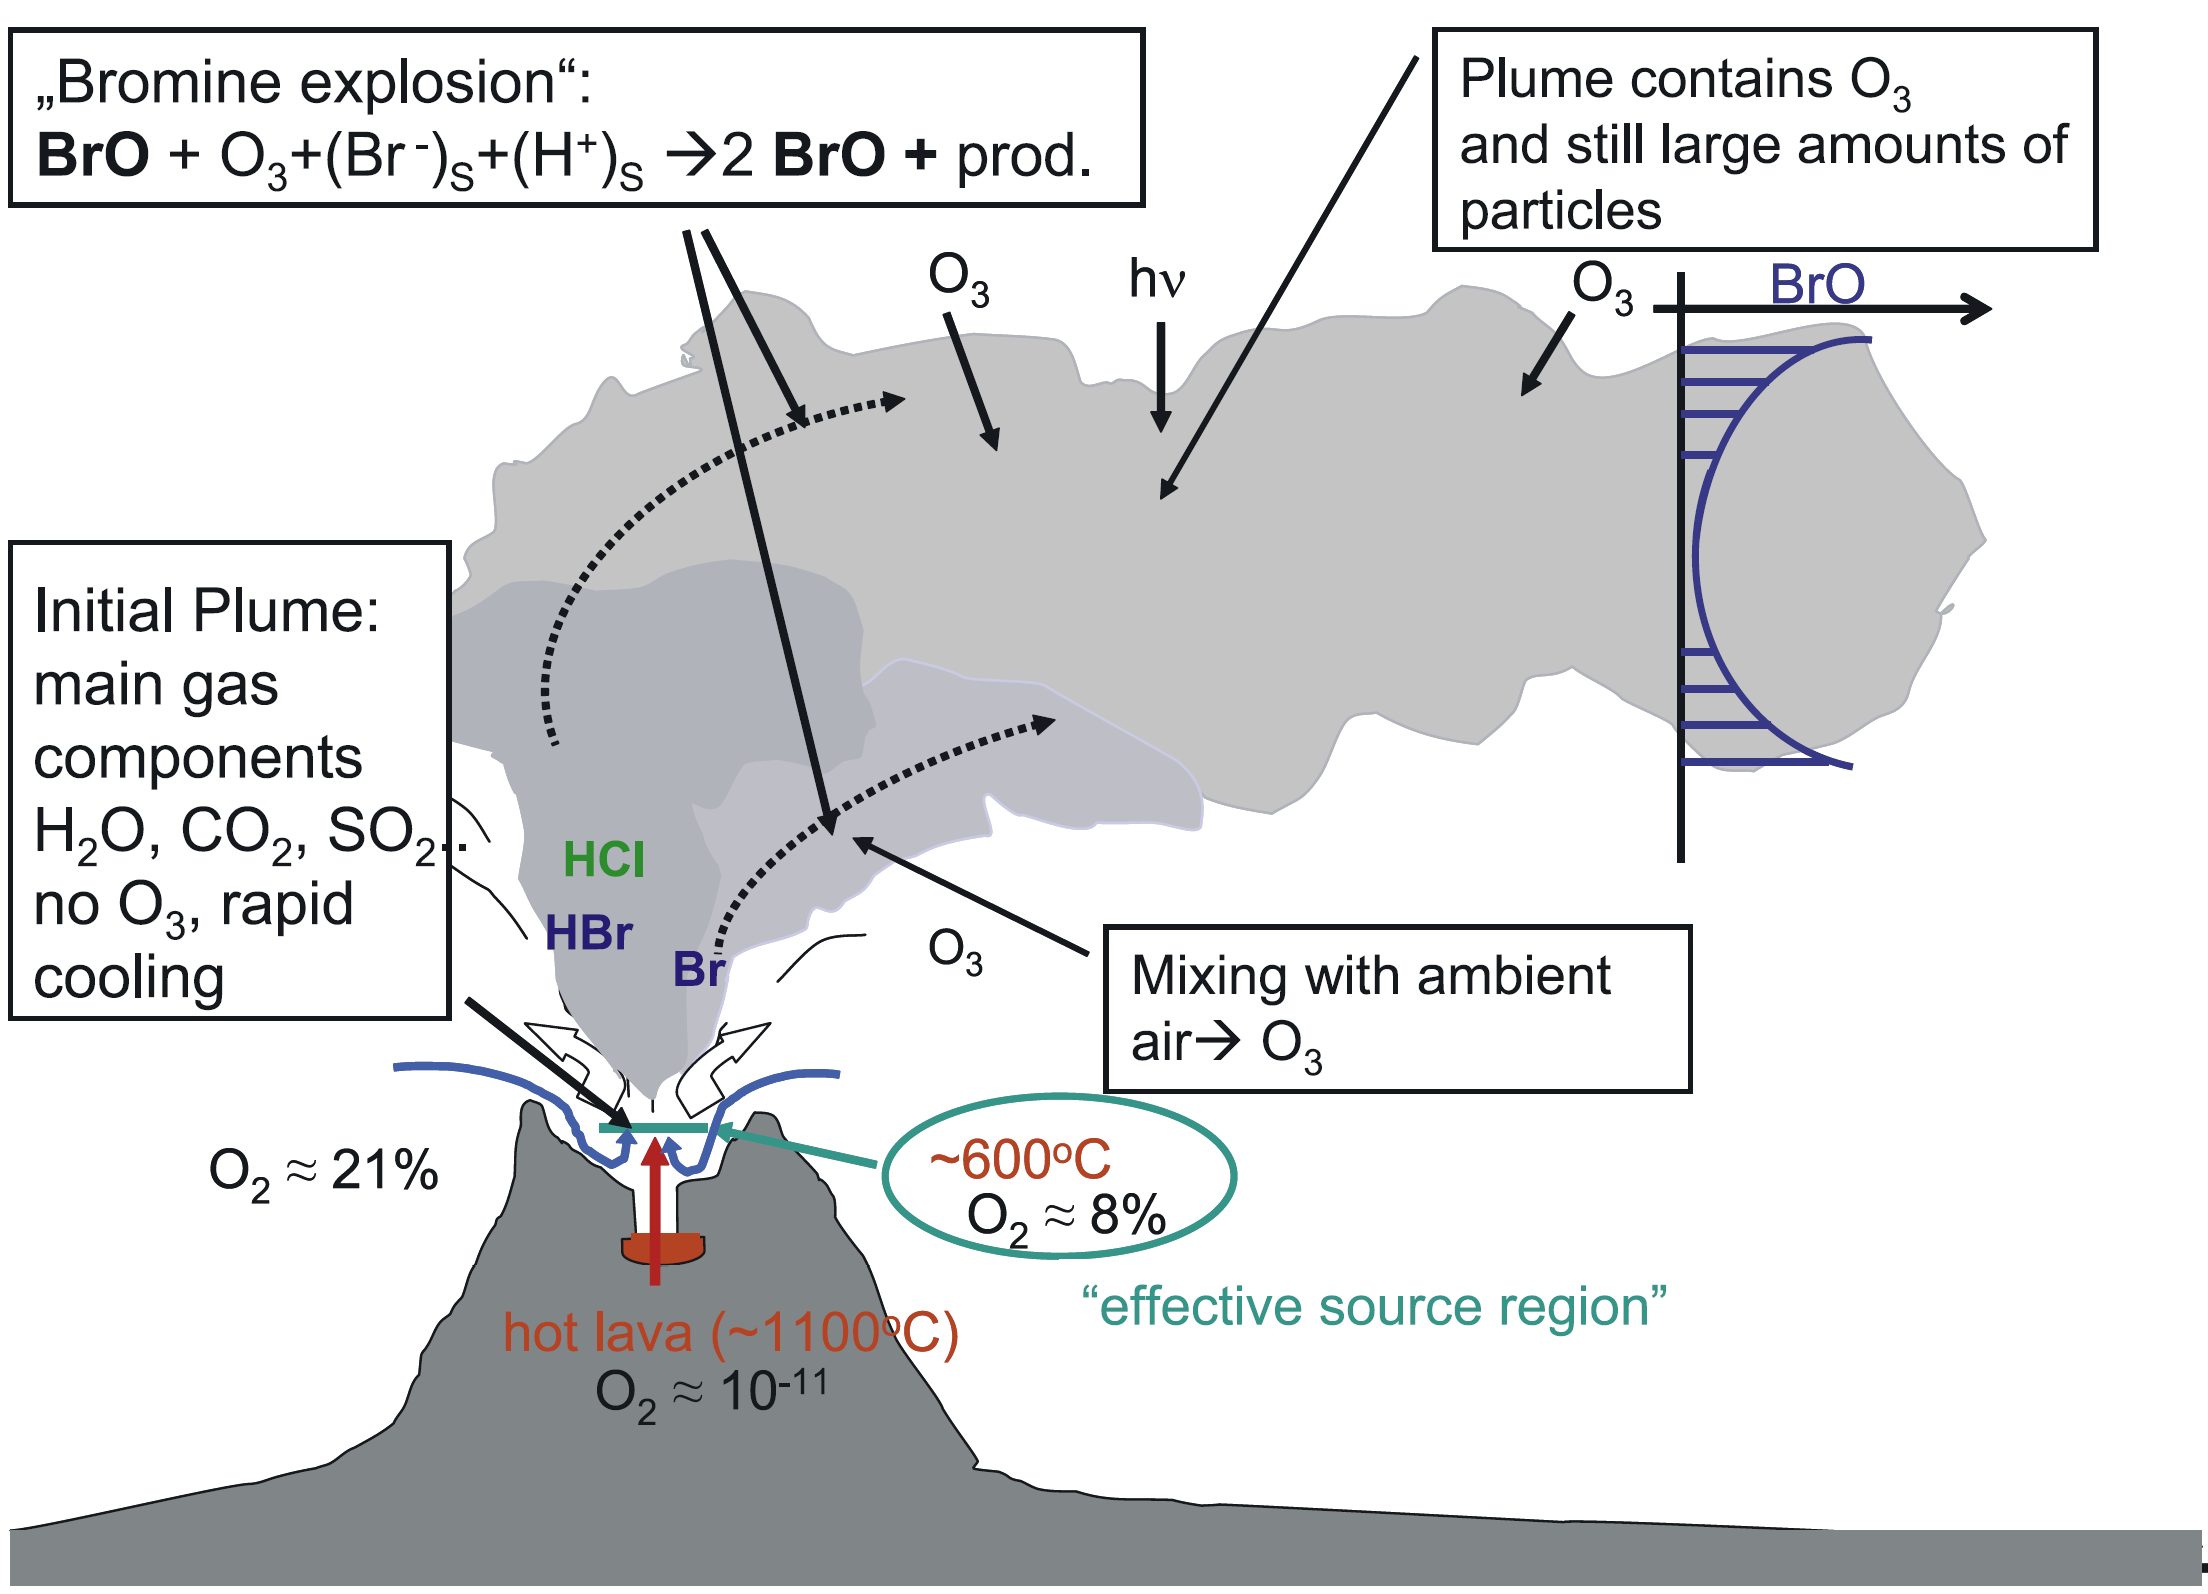
\includegraphics[width=0.8\linewidth]{Bilder/Simon/Bilder_Tung/BrO_Plume}
\caption[schematic sketch of a bromine Explosion. Adapted from \citet{bobrowski2007reactive}.]{schematic sketch of a bromine Explosion.
	Release of \ce{HBr} at the volcanic vent. Mixing with ambient air in the effective source region leads to \ce{Br} formation. This resulting bromine species react to \ce{BrO} with ozone from the plume. Adapted from \citet{bobrowski2007reactive}}
\label{fig:broplume}
\end{figure}
The amount of bromine in volcanic plumes is rather low compared to \ce{SO2}. The first time bromine monoxid (BrO) was observed at a volcano was 2013 at the soufriere hills by \citet{bobrowski2003detection}. Since then many others were able to detect \ce{BrO}  using ground based remote sensing measurement techniques (DOAS: see \cref{DOAS}) for example:
\citet{bobrowski2007so2}, \citet{bobrowski2007reactive},\citet{vogel2011volcanic} and \citet{lubcke2014bro}
\\
The main bromine formation which is released from the volcano is  \ce{HBr}. \ce{BrO}  is formed due to mixing with the ozone rich atmosphere at ambient temperatures \citep{bobrowski2007reactive}.\\
Due to the raising of hot air in the volcano vent , ambient air is pulled into the vent. There temperatures of  600$^{\circ}$C to 1200$^{\circ}$C    prevent the formation of \ce{BrO}. Only Br is formed. \ce{BrO}  occur after further cooling and mixing while rising. When the temperature cooles down to ambient conditions the so called "Bromine Explosion" causes a non linear formation of \ce{BrO}.
The "Bromine Explosion" is illustrated in \cref{fig:broexplosion} and can be described with the following reaction cycle:
\begin{align}
\ce{HBr}_{gas} &\rightarrow \ce{Br}^{-}_{aq} + \ce{H}^{+}_{aq} \label{eq1}\\
\ce{HOBr}_{(gas)} &\rightarrow \ce{HOBr}_{(aq)} \\
\ce{HOBr}_{(aq)} + \ce{Br}^{-}_{(aq)} + \ce{H}^{+}_{(aq)} &\rightarrow
\ce{Br}_{2(aq)} +  \ce{H2O}\label{eq2}\\
\ce{Br}_{2,aq} &\rightarrow \ce{Br}_{2,gas} \\
\ce{Br2} + h\nu &\rightarrow 2 \ce{Br} \\
\ce{Br} + \ce{O3} &\rightarrow \ce{BrO} + \ce{O2} \\
\ce{BrO} + \ce{HO2} &\rightarrow \ce{HOBr} + \ce{O2} \\
\ce{BrO} + \ce{BrO} &\rightarrow 2 \ce{Br} + \ce{O2} \\
\ce{BrO} + \ce{BrO} &\rightarrow \ce{Br2} + \ce{O2}
\end{align}
The gaseous \ce{HBr} emitted by the volcano is split heterogeneously int H$^{+}$ and Br$^{-}$ (\cref{eq1}). Inside of an aerosol it forms with HOBr \ce{Br2} and \ce{H2O} (\cref{eq2}). \ce{Br2} evaporates to the gaseous phase and splits photolytic  into 2Br. Including an ozon molecule (\ce{O3}) the two Br react to 2BrO. The last step o the circle visualized in \cref{fig:broexplosion} with blue lines is the reaction of a BrO with \ce{H2O} to an HOBrO molecule condensing into the liquid phase  and thuse closing the circle. The non linear explosion occurs due the formation of two BrO particles from one \ce{Hbr} from the volcano.\\
The BrO formation is slightly diminished due to self reaction of BrO molecules marked with the red lines in \cref{fig:broexplosion}. The 2BrO react with themselves and form \ce{Br2} or may split photolyticaly into 2Br.\\
The BrO concentration reaches a maximum approximately five to ten minutes after emission and then remains constant for the next 25 minutes \citep{lubcke2014bro}.
 %
\begin{figure}
	\centering
	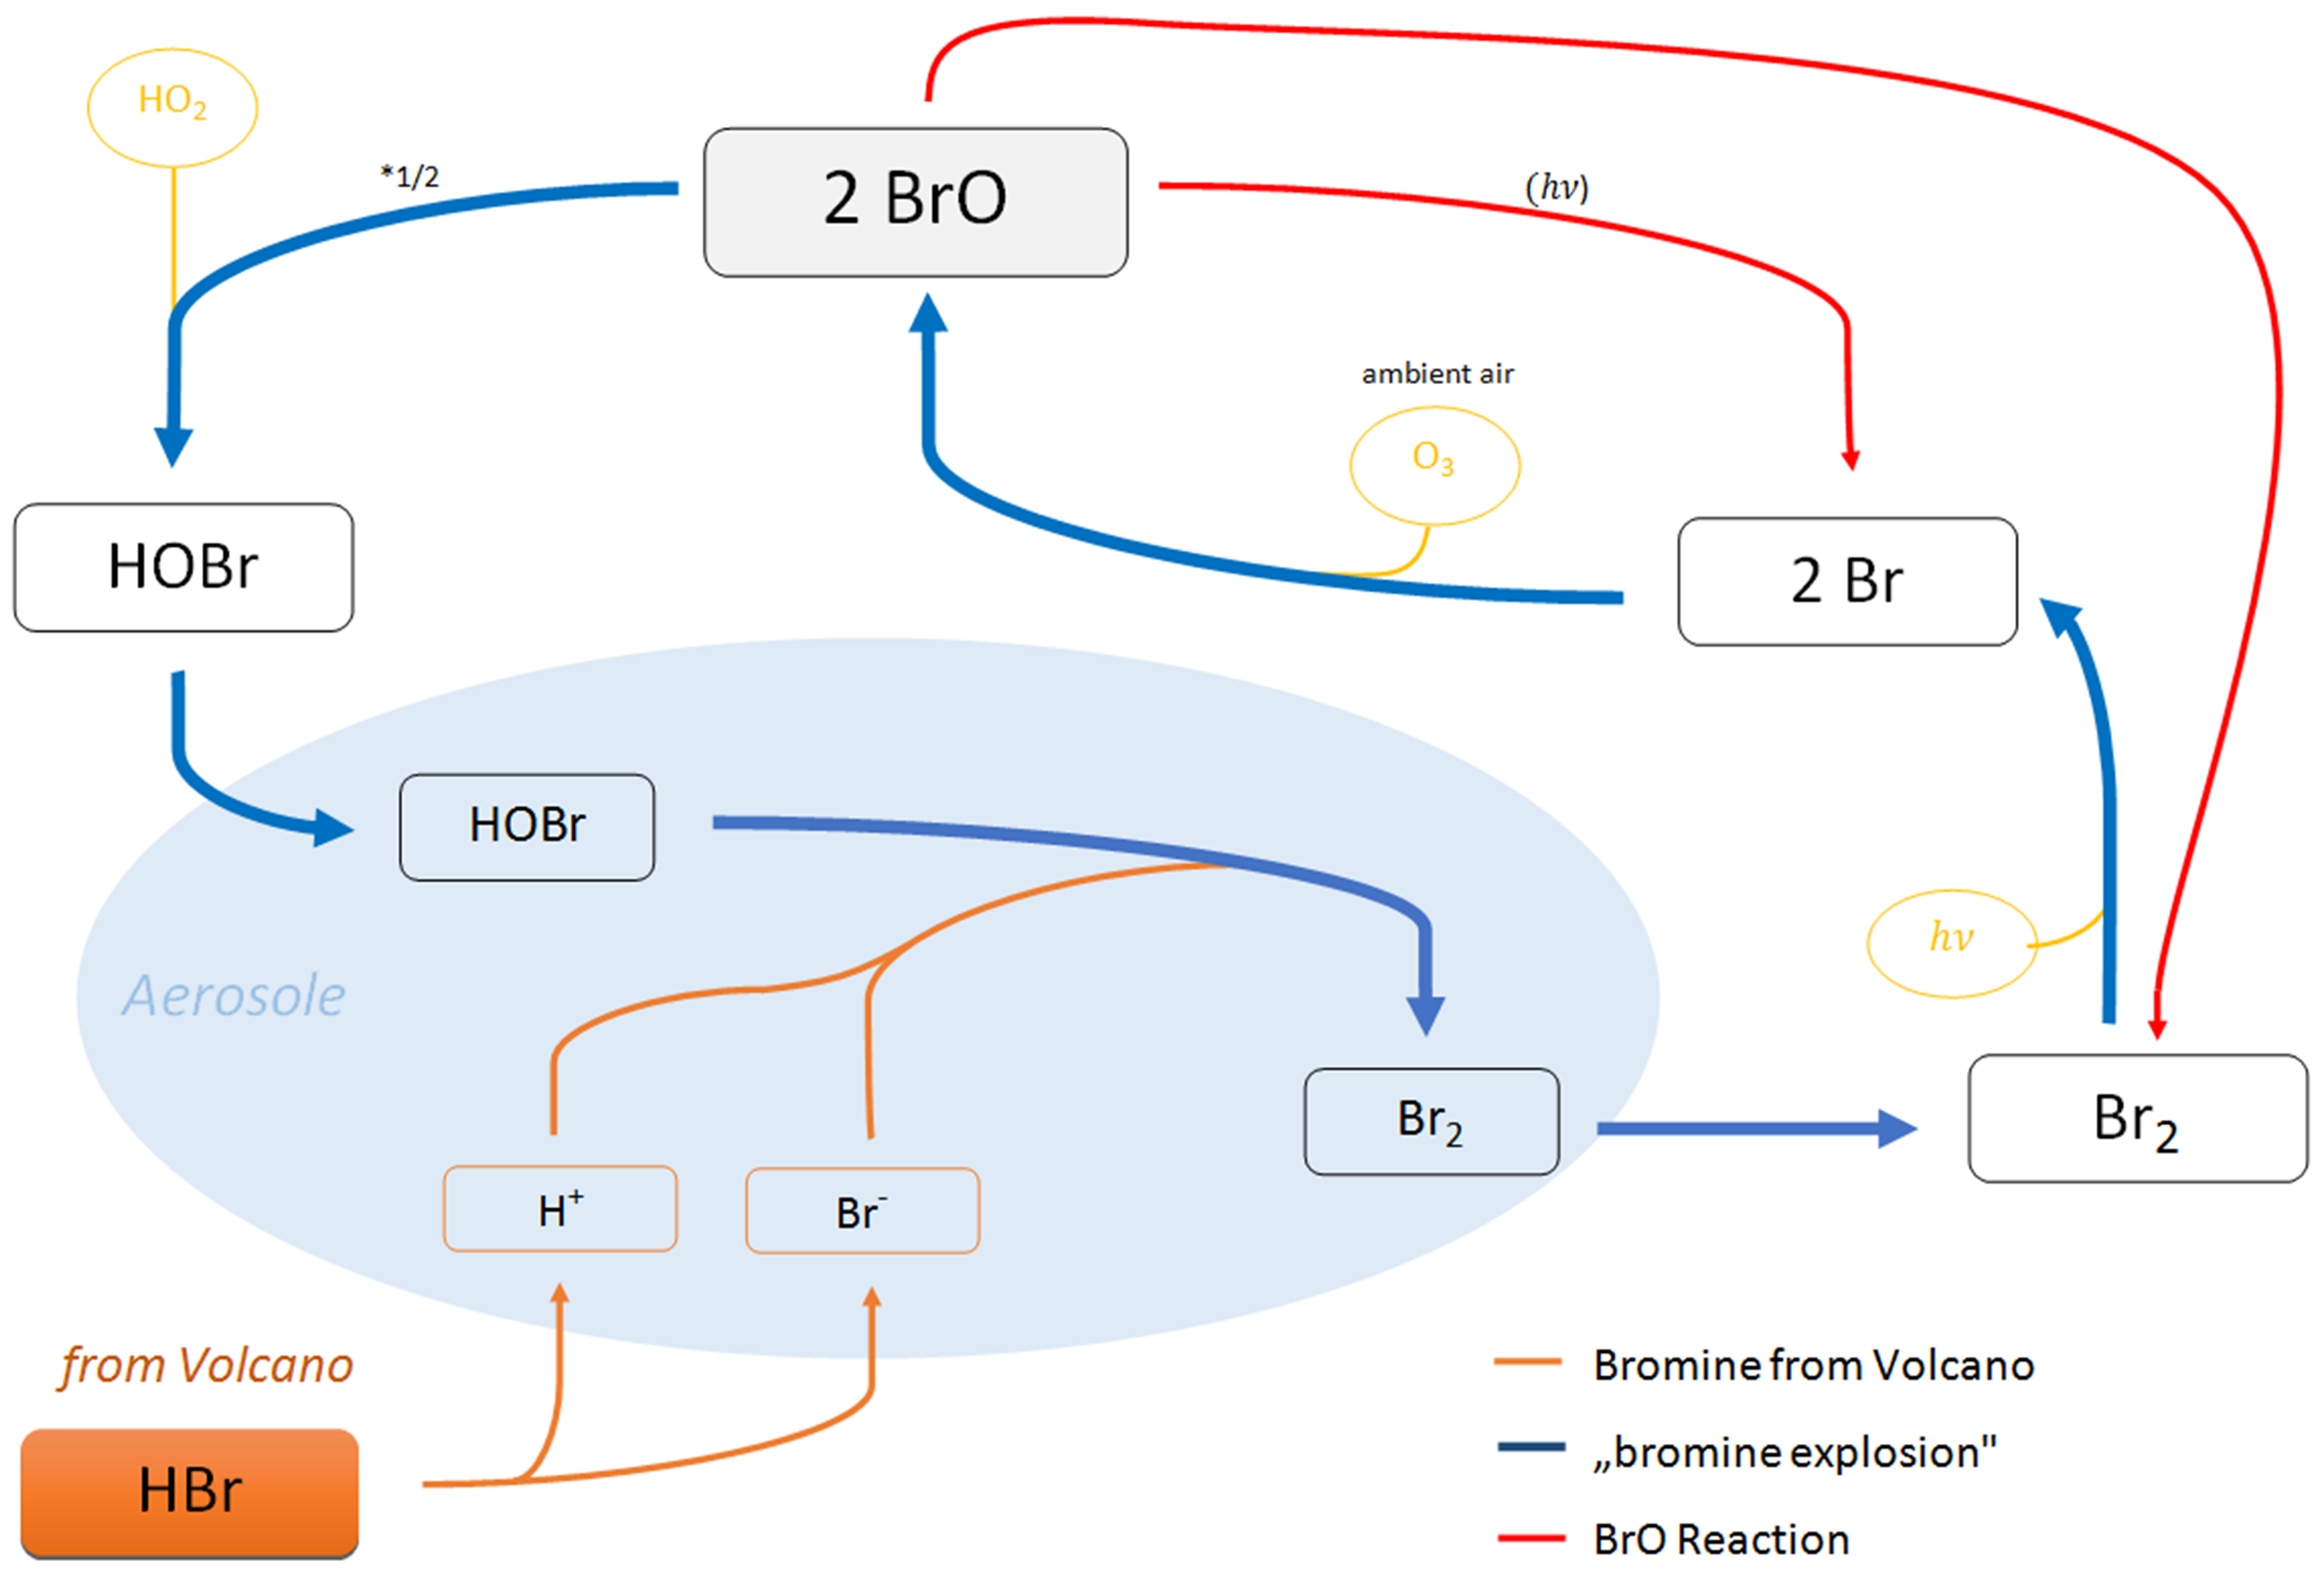
\includegraphics[width=0.7\linewidth]{Bilder/Simon/Bilder_Tung/BrO_Explosion}
	\caption[Bromine reactions inside of a volcanic vent. From \citet{WarnachSimon}.]{Bromine reactions inside of a volcanic vent. The release of \ce{Hbr} at the volcaninc vent is drawn  in orange. Inside of aerosols heterogeneous dissociation with HOBr forms \ce{Br2}. Then \ce{Br2} splits photolytically into single Br radicals. \ce{BrO}  results through a reaction with  \ce{O3}upon mixing with ambient air. Reactions with  \ce{H2O}  forms \ce{HOBr} creating an autocatalytic cycle. The reaction cycle along the blue lines are called bromine explosion. From \citet{WarnachSimon}.}
	\label{fig:broexplosion}
\end{figure}
%
\section{Using the \ce{BrO}/\ce{SO2}  ratio to study volcanic activity}
\begin{figure}
	\centering
	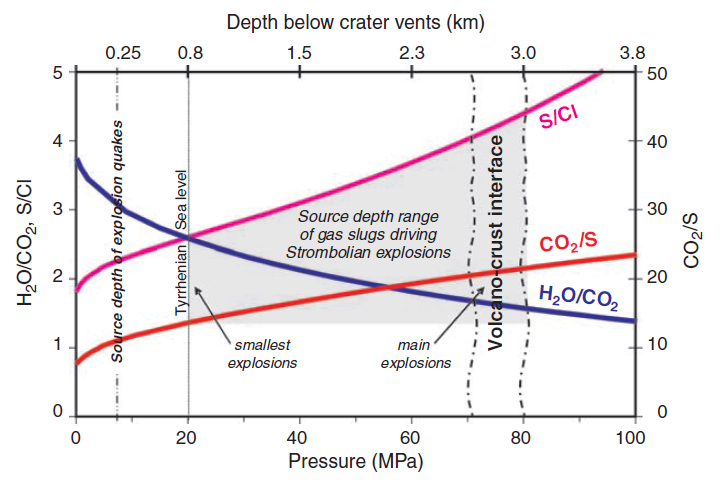
\includegraphics[width=0.9\linewidth]{Zwischenbericht2018/Bilder/so2_bro}
	\caption{Dependence of the ratios of different volcanic trace gases on depth. Data originate from Stromboli volcano. From \citet{lubcke2014optical} reproduced from Burton et al. (2007)}
	\label{fig:so2bro}
\end{figure}    
	Volcanic degassing is influenced by many factors, which can be exploit to study volcanic activity by using the gas composition of the volcano plume. Therefore remote sensing should be an additional tool for forecasting of volcanic activity next to classical monitoring techniques like seismographic and deformation measurements.\\
	Inside of volcanoes volatiles are in solution in magmatic melt. The Henry law shown in \cref{Henrylaw} describes the necessary conditions for gas formation:
	\begin{equation}
	P = K_{H}\cdot c
	\label{Henrylaw}
	\end{equation}
	Here P is the partial pressure at equilibrium of the solute, c is the concentration and $ K_{H}$ is the Henry constant which is anti proportional to the solubility $\alpha$ ($\alpha = \frac{1}{ K_{H}}$).
	If the partial pressure of the gas solute (in this case a magmatic gas constituent) exceeds the pressure of the surrounding solvent, a formation of gaseous bubbles occur. Otherwise, if the partial pressure of the gas in the solution is below the surrounding pressure the formation of gas bubbles stops.\\
	The solubility $\alpha$ depends on the temperature, the chemical composition and on the solvent (here magma). Whereas the partial pressure of the constituent depends on the surrounding pressure. The pressure below the volcanic vent increases with depth. This leads to a correlation between the partial pressure of the constituents and the depth.
	The result is, that the gas starts exsolving at a certain depth depending on the  partial pressure of the constituent. Thus, the gas bubble formation increases with rising magma. But at a certain depth the percentage of solved gas is different for each volcanic gas. The result is, that the composition of the gases changes with depth. So gas ratios contain information about its originating source depth.\\
	Prior to volcanic eruptions the magma starts raising. Since the gas is mostly less dense than the magma, it raises faster and could therefore be an indicator for its origin source depth and thus an indicator for the volcanic activity.\\
	\Cref{fig:so2bro} shows the empirical measured ratios of  \ce{H2O}/\ce{CO2}, S/CL, \ce{CO2}/S as a function of the pressure respectively on the depth.
	%
	\citet{noguchi1963prediction} found a decrease of Cl/S prior to eruptive periods
	%
	\citet{pennisi1998variations} observed a lower CL/S ratio during eruptive periods compared to non eruptive periods at Mt. Etna.
	%
	\citet{burton2007magmatic}  found \ce{CO2}/\ce{SO2} and \ce{SO2}/hCl ratios 3-5 times higher during explosions  compared to quiet degassing episodes.
	%
	 \begin{figure}
		\centering
		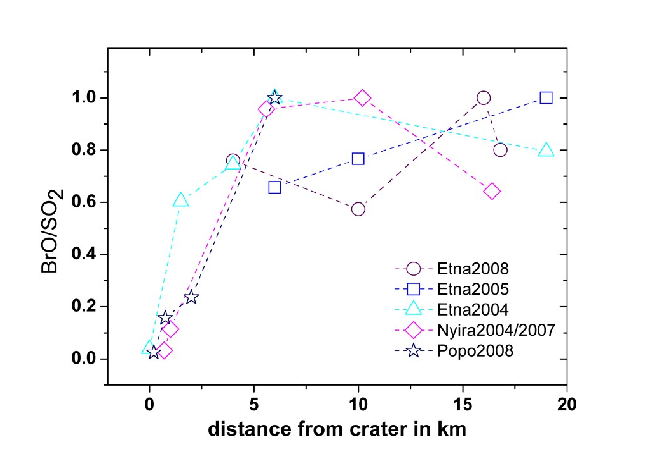
\includegraphics[width=0.7\linewidth]{Bilder/rat_diff}
		\caption{BrO/\ce{SO2} ratio as a function of the distance from the volcanic vent with a constant wind speed of 10 m/s. From \citet{lubcke2014optical}.}
		\label{fig:ratdiff}
	\end{figure}	
	The authors compared these data to gas formation simulations for different degassing source depth, they concluded that these eruptions were driven by gas slugs from deeper levels where the ratios were higher while quiet degassing originates from from shallow magma.\\
	%
	Especially halogen-sulfur ratios are interesting as possible tracer for the volcanic activity since the ambient air concentrations are negligible.
	BrO/\ce{SO2}  curves equivalent as in \cref{fig:so2bro} are yet not available due to lack of  bromine solubility curve but the following observations are made:
	%
	Changes of \ce{BrO}/\ce{SO2}  are found by \citet{bobrowski2006bromine}: multiple eruptions between 2006 and 2009 highest ratios 2-3 month before the eruptions the ratio then decreased and was lowest during eruptive phase. Therefore it could be concluded that bromine exsolves earlier, at lower depth than sulphur.
	%
	\citet{lubcke2014bro} found decrease of \ce{BrO}  5 month prior to the eruption 2012 at Nevado del Ruiz which also can be attributed to a earlier exsolution of bromine during rising magma.
	%
	Despite the lack of the solubility curve of \ce{BrO}  until now, the \ce{BrO}/\ce{SO2}  has a great potential for investigations of the volcanic activity. The first reason is, that both gases can be measured with remote sensing by DOAS instruments. For examples ground based measurements by \citet{bobrowski2007reactive}, \citet{lubcke2014optical} or satellite based measurement by \citet{hormann2013systematic} or \citet{beirle2014estimating}. The advantage of remote sensing techniques is the possibility of measuring during eruptions which is with in situ measurements not always possible.
	Secondly due to the NOVAC network (See \cref{NOVAC}) continues measurements are possible.\\
	Another reason for the research on \ce{BrO}/\ce{SO2}  ratios at volcanoes is that the ratio is almost constant from 5 to at least 30 minutes after release \citep{bobrowski2007reactive};\citep{lubcke2014optical}. Furthermore \cref{fig:ratdiff} shows a almost constant ratio from 5 to 20 km off the volcano. This ensures that the data measured from different positions or at different conditions are comparable.\\
	\\
	\subsection*{Volcanic gases and their impact on the climate}
	\begin{figure}
		\centering
		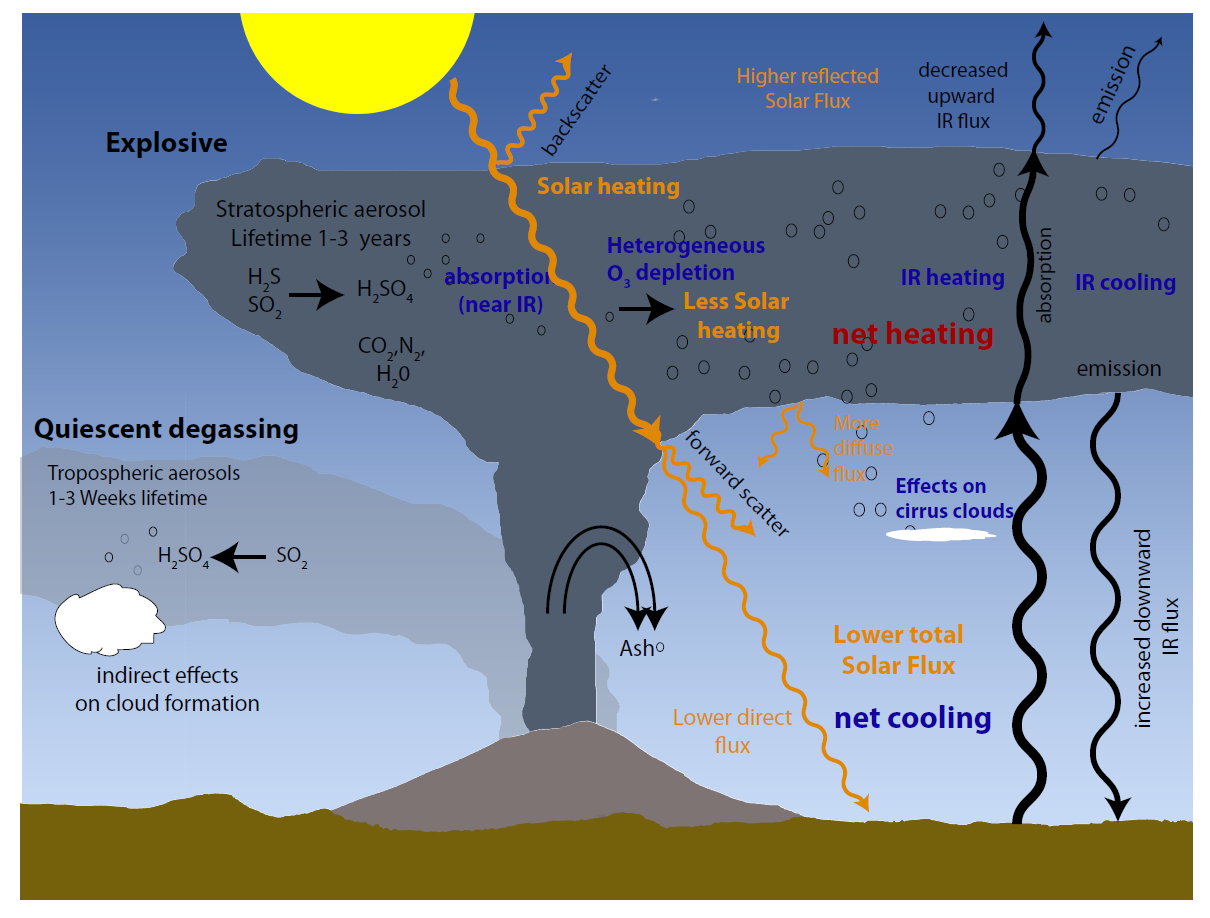
\includegraphics[width=0.8\linewidth]{Bilder/Simon/Bilder_Tung/Climate_Influence}
		\caption{Influence of volcanic eruptions and quiet degassing on earth climate. Redrawn on the basis of \citet{robock2000volcanic}}
		\label{fig:climateinfluence}
	\end{figure}
	Volcanoes emit various gases (see \cref{tab.volcemissions}) in the atmosphere. This can occur due to volcanic eruptions or due quiet degassing. Gas emitted by quiet degassing remains in the troposphere while eruptions can inject volcanic gases up to the stratosphere \citep{robock2000volcanic}. The larger lifetime in the stratosphere and a larger sensitivity of the stratospheric chemistry to volcanic gases leads to an higher impact on the earth climate of these gases.
	Volcanic gases have a large influence on the earth climate especially \ce{CO2} and \ce{SO2}  or more specific its oxidation product sulfur acid.\\ 
	The relevance of  \ce{CO2} for the climate is a subject of many discussions about the climate change. Compared to other atmospheric \ce{CO2} sources, the share of volcanic  \ce{CO2} is rather low.\\
	\\
	Even though the \ce{SO2} emissions during eruptive episodes are up to one order higher than during quite degassing episodes, \citet{halmer2002annual} estimates that quiescent degassing contributes 40\% of the accumulated \ce{SO2} between 1972 to 2000.\\
	\citet{halmer2002annual} estimated the mean annual \ce{SO2}  emitted from volcanoes from 1972 to 200 as 7.5 to 10.5TgSyr$^{-1}$, while the anthropogenic \ce{SO2}  amount for 2000 is estimated as 55 TgSyr$^{-1}$ \citep{IPCC}. Despite the less \ce{SO2}  occurring from volcanoes the impact may be higher as the impact of the anthropogenic \ce{SO2}. \citet{graf1997volcanic} supposed that the volcanic \ce{SO2}  has a higher impact on the climate since its reaches up to the stratosphere while the anthropogenic \ce{SO2}  is mostly located in planetary boundary layer. In the lower troposphere sulphuric acid has a lifetime of about a week whereas the lifetime in the stratosphere is about a year \citep{IPCC}.\\
	Sulphuric acid in the atmosphere increases the earth albedo due to direct backscattering radiation. Additional the condensation on sulphuric acid particles leads to finer droplets and thus to more stable and more white clouds. This increases the albedo as well \citep{twomey1974pollution}.
	Volcanic particles can be surfaces for heterogeneous reaction. The result is a depletion of stratospheric ozone, and thus a more high energetic solar flux on the earth surface.
	Large particles may backscatter IR radiation from the earth surface and the lower atmosphere, leading to a small reduction of the net cooling of the lower troposphere.
	In the upper troposphere or stratosphere absorption of IR or UV radiation results in a net heating in the stratosphere and a cooling at the earth surface.
	\Cref{fig:climateinfluence} shows the above described effects and their localization in the atmosphere.
	The dominating radiative effect of volcanic gases is a cooling of the earth atmosphere due to  more backscattered radiation, more diffusive scattering\citep{robock2000volcanic}.
	\citet{IPCC} records a volcanic radiative forcing of $-0.11W/m^{2}$ between 2008 and 2011. For comparison the radiative of  \ce{CO2} is estimated as  $1.68W/m^{2}$.
%	This chapter motivated the research on the \ce{BrO}/\ce{SO2}  ratio as a tracer for volcanic activity.
	
	\chapter{Network for Observation of Volcanic and Atmospheric Change \label{NOVAC}}
%	
	

%% NOVAC
%% =============
%%
		\begin{figure}[h]
			\centering
			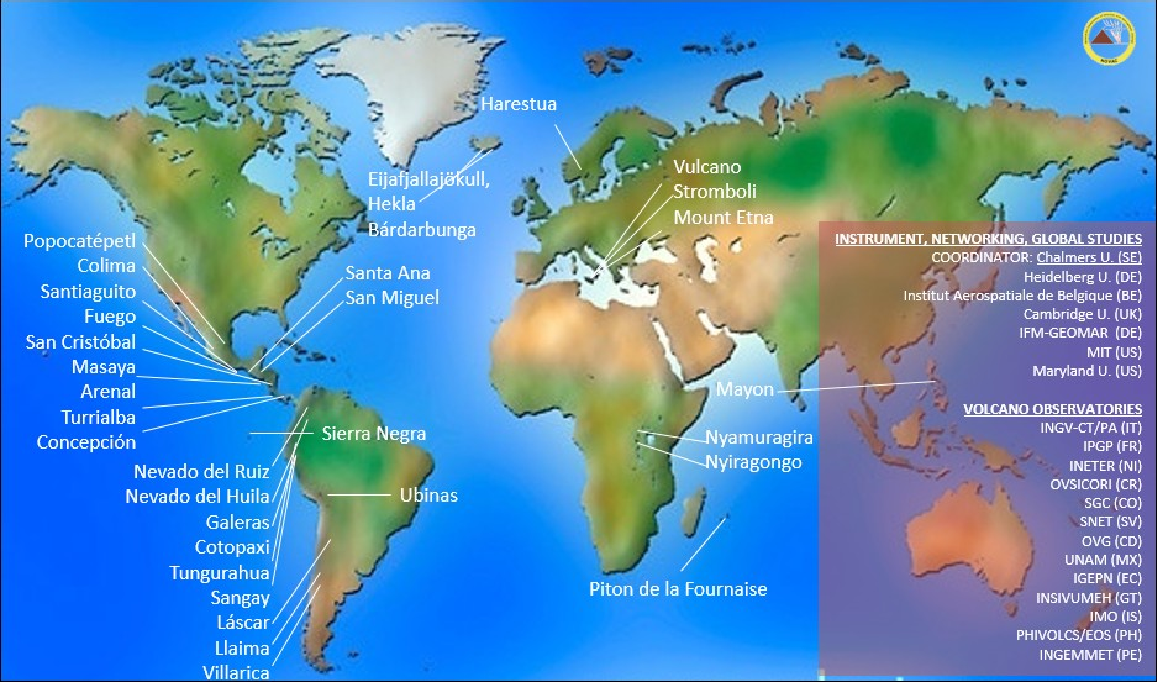
\includegraphics[width=0.8\linewidth]{Bilder/NOVAC2015}
			\caption{Global map of the volcanoes monitored by NOVAC. Used with friendly permission of Santiago Arellano.}
			\label{fig:novac2015}
		\end{figure}
		Network for Observation of Volcanic and Atmospheric Change (NOVAC) is a network of instruments monitoring volcanoes over the whole world. 
		%
		The aim of NOVAC is to gain another tool for risk assessment, for gas emissions and geophysical researches. Also many other scientific purposes are build on the data from NOVAC.\\
		%
		NOVAC was originally funded by the European Union on the first October in 2005. The aim of NOVAC is to  establish  a  global  
		network  of  stations  for  the  quantitative  measurement  of  volcanic gas  emissions. At the beginning, NOVAC encompassed observatories of 15 volcanoes in Africa America and Europe, including some of the most active and strongest degassing volcanoes in the world. Although the EU-funding has stopped, the network has been constantly growing since it was founded. In 2017 more than 80 Instruments are installed at over 30 volcanoes in more than 13 countries.
		\Cref{fig:novac2015} shows a map, with all volcanoes of the Network for Observation of Volcanic and Atmospheric Change.\\
		
		The great advantage of the data monitored in NOVAC is the fact
		that NOVAC provides continues gas emission data over many years. This ensures statistically meaningful results for the data evaluation.\\
		The instruments used in NOVAC are scanning UV-spectrometer named Mini Doas instruments. \\
		The  Mini DOAS  instrument  represents  a  major  breakthrough  in  volcanic  gas	monitoring as it is capable of real-time semi-continuous unattended measurement of the total emission fluxes of  \ce{SO2} and BrO from a volcano. Semi-continues in this case means that the measurement is only possible during daytime when enough Sunlight is there.\\
		%
		\begin{figure}
			\subfigure[Bezeichnung der linken Grafik]{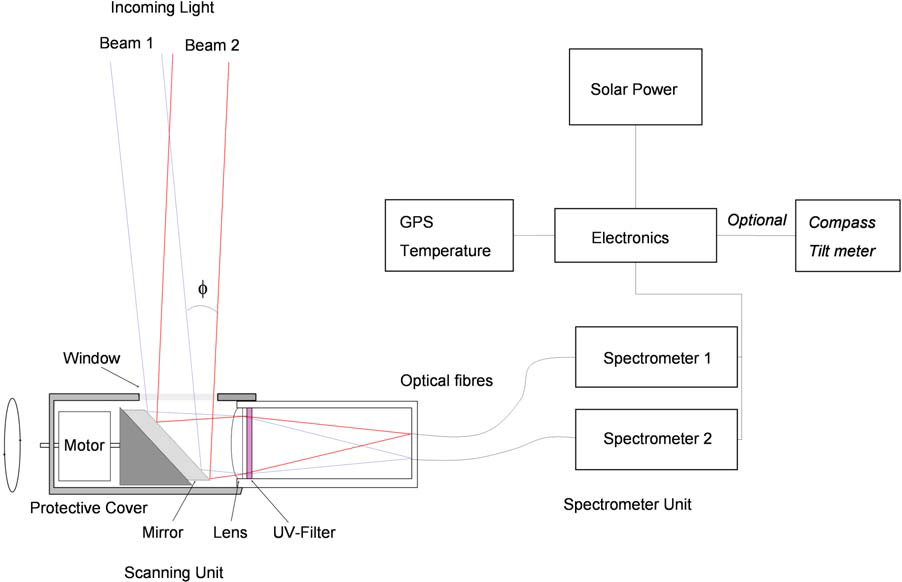
\includegraphics[width=0.49\textwidth]{Bilder/Simon/Bilder_Tung/NOVAC_Instrument}}
			\subfigure[Bezeichnung der rechten Grafik]{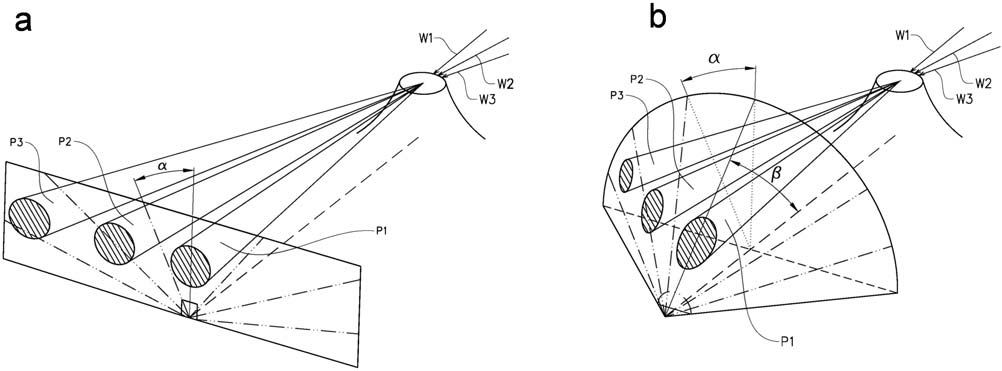
\includegraphics[width=0.49\textwidth]{Bilder/Simon/Bilder_Tung/NOVAC_scan_geo}}
			\caption{Titel unterm gesamten Bild}
		\end{figure}
		The  basic  Mini DOAS  system  consists  of  a  pointing  telescope  fiber-coupled  to  a  spectrograph.  
		Ultraviolet light from the sun, scattered from aerosols and molecules in the atmosphere, is collected by 
		means  of  a  telescope  with  a  quartz  lens  defining  a  field-of-view  of  12~mrad.
		\cite{NOVACsite} \\
		The spectrometers measure in the UV region in a wavelength range of 280 to 420~nm. In this range the differential structures of \ce{SO2} and BrO are dominant.
		\\
		The NOVAC-instruments need to be very robust to stand the conditions around volcanoes. Therefore the design of the instruments is rather simple, this means the instruments do not have internal stabilisation features like temperature stabilization to keep the measurement independent of external parameters.\\
		This comes with a reduced precision of the data, but the huge amount of data produced by NOVAC compensates for this limitation.  
		
		
		\section{Measurement Routine}
		\begin{figure}[h]
			\centering
			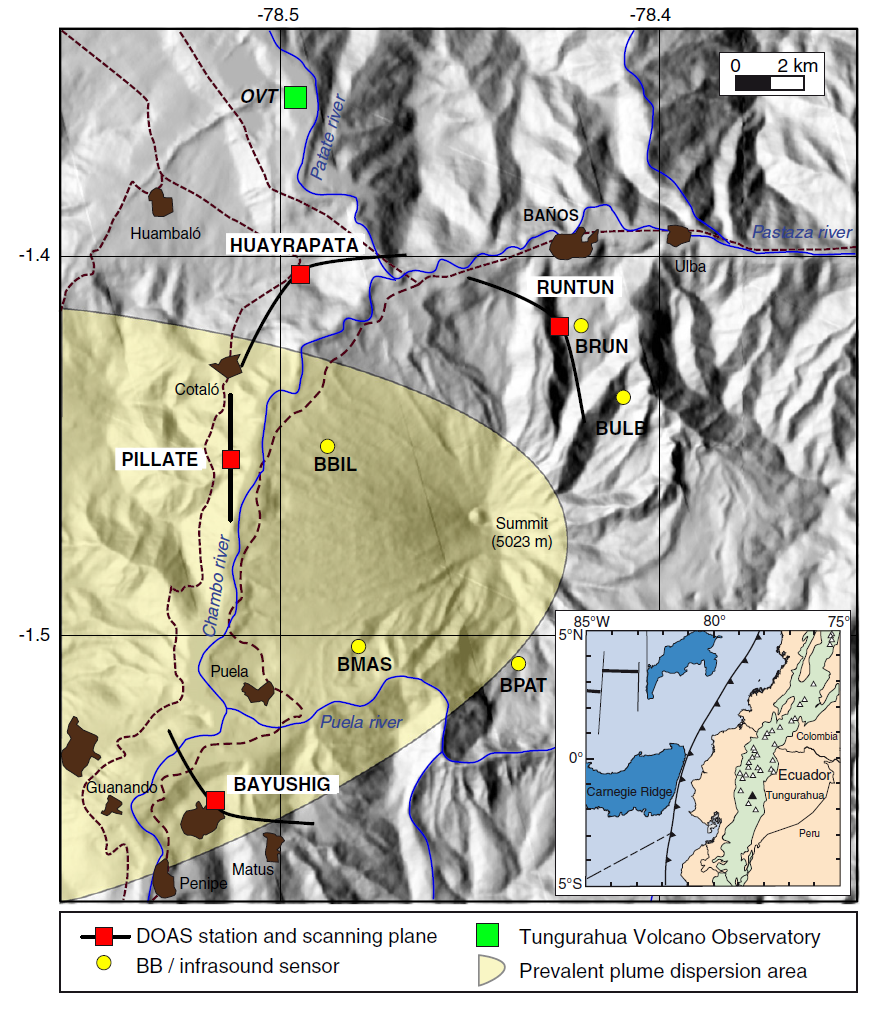
\includegraphics[width=0.6\linewidth]{Bilder/Simon/Bilder_Tung/Map_Tungurahua2}
			\caption{}
			\label{fig:maptungurahua2}
		\end{figure}
		The Instruments are set up five to ten km downwind of the volcano. To cover most of the occurring wind directions two to five instruments are installed at each volcano. Ideally, the measurement plane is orthogonal to the plume, to get the best measurement results. In reality, the measurement plane might be rotated.\\
		The Instruments record spectra in different viewing angles covering a the hole sky from horizon to horizon.\\
		The zenith is at 0$^{\circ}$.
		The measurement routine starts with a spectrum in zenith direction: the pre-reference.
		Afterwards, the dark current spectrum is recorded.\\
		Then the Instrument turns automatically to the side, recording spectra at the elevation angle from -90$^{\circ}$ to 90$^{\circ}$ with steps of 3.6$^{\circ}$. \\
		One hole measurement takes 6 to 15 minutes.
%
	\chapter{Remote sensing of volcanic gases}

	In this thesis we are interested in the volcanic trace gases \ce{SO2} and \ce{BrO}, both measured with the Differential Optical Absorption Spectroscopy (DOAS) a remote sensing technique proposed by \citet{platt1980observations}

	

	\section*{Beer-Lambert Law}
	The Beer-Lambert law describes the attenuation of light when travelling through a material.\\
	This section will give an overview about the reasons for decreasing light intensity when going through a medium.\\
	The Beer-Lambert law describes the attenuation of light when travelling through a material.\\
%
	Atoms and molecules exists in several energy states, depending on the different electron configuration. Moreover molecules have additionally rotation and vibration states, also enclose to the energy states. If a photon energy matches the energy gap between two possible energy states, this includes, that the lower energy state is occupied and the selection rules are fulfilled  the molecule could absorb the photon, remaining in a higher energy state.\\
	The additional energy could be loosed by collision with another molecule or by emission. But since the direction of the emitted photon is mostly not the same direction of the absorbed photon the intensity I$_{0}$ of the light before passing the medium is higher than the intensity I after travelling the distance L through the medium.\\
	This can be described as:\\ 
	\begin{equation}
	I\left(L,\lambda\right) = I_{0}\left(\lambda\right)\cdot exp\left(-\int^{L}_{0}\sigma\left(\lambda,p(l),T(l)\right)\cdot c\left(l\right)dl\right)
	\end{equation}
	where $\lambda$ is the wavelength,$c\left(l\right)$ is the location-dependent concentration of the trace gas of interest. $\sigma\left(\lambda,p,T\right)$ is the absorption cross section, $\sigma\left(\lambda,p,T\right)$ is unique for each molecule and depends on pressure p and on the temperature T.\\
	%
	An important quantity used in many optical remote sensing techniques is the optical density $\tau$. The optical density is a measure for the weakening of radiation when going through a material. At a volcano the variation of temperature and pressure in different viewing angles is negligible, thus, $\sigma\left(\lambda,p(l),T(l)\right)$ is independent of $l$ required to consider it within the integral. Then  $\tau$ can be calculated using the Beer-Lambert law:
	\begin{equation}
	\tau = ln\left(\frac{I_{0}\left(\lambda\right)}{I\left(\lambda\right)}\right) = \sigma\cdot S
	\end{equation}
	With $S$ is the column density. $S$ can be calculated as:
	\begin{equation}
	S = \int_{0}^{L}c\left(l\right)dl
	\end{equation}
	The column density is the concentration of the trace gas when integrating along the light path, the dimension of $S$ is therefore the number of molecules divided by an area: $\frac{\text{molec}}{\text{cm}^2}$.\\
	%
	\begin{figure}
		\centering
		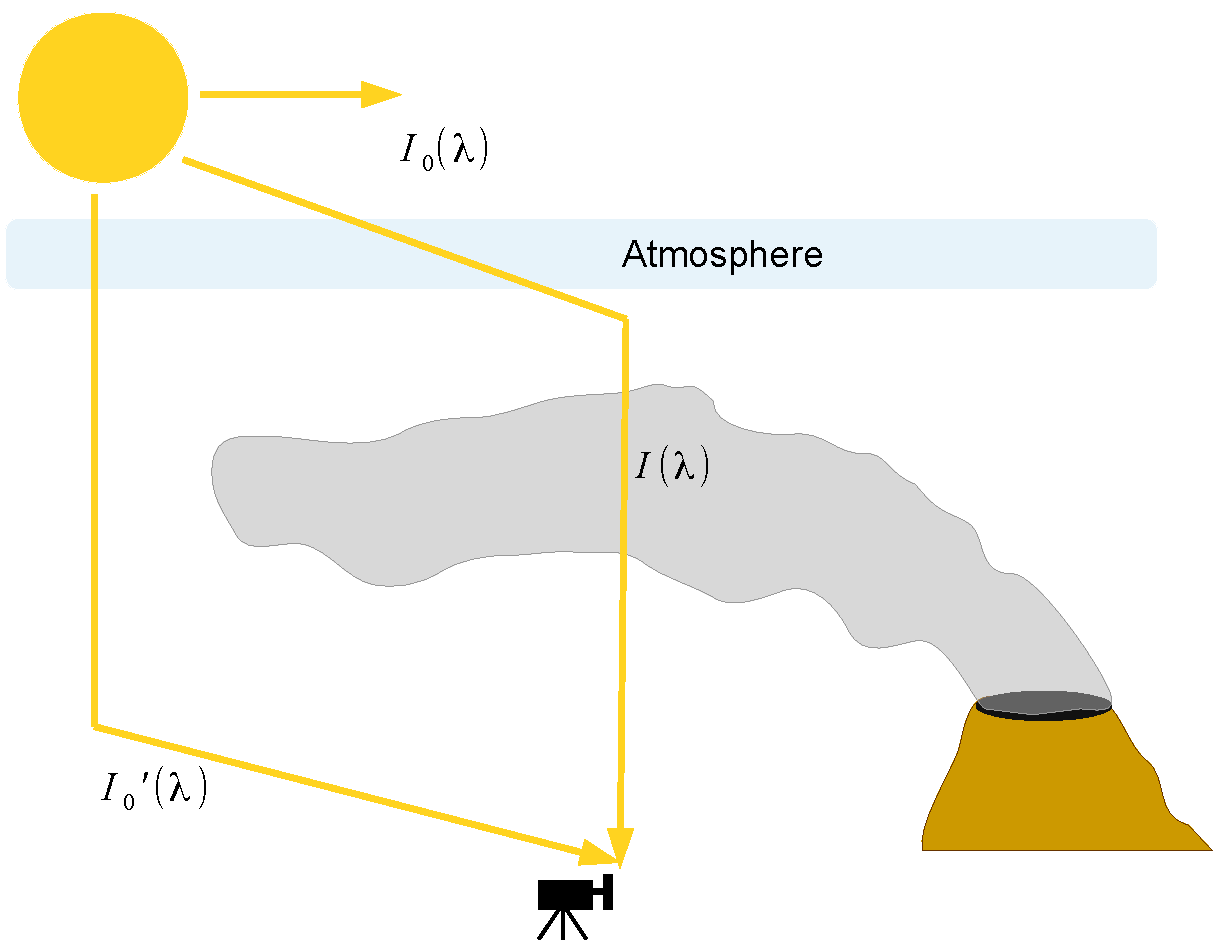
\includegraphics[width=0.7\linewidth]{Bilder/DOASFunction}
		\caption[Schematic sketch of the DOAS measurement of volcanic plume constituents.]{Schematic sketch of the DOAS measurement of volcanic plume constituents. The column density of the plume constituent of interest is retrieved by comparing the spectrum $I\left(\lambda \right)$ which is measured through the plume with the spectrum  $I_0^{'}\left(\lambda \right)$ measured outside of the plume.}
		\label{fig:doasfunction}
	\end{figure}
	
	When measuring in atmosphere, the situations gets more complex, since one need to deal with several absorbers and scattering processes have to be taken into account. 
	Scattering processes in the atmosphere can be roughly grouped in Rayleigh scattering, scattering at very small particles and Mie scattering, scattering at larger particles (radius$\approx \lambda$). The effects on the spectrum caused by scattering need to be considered in the calculations.  One possibility is to treat scattering effects as pseudo absorbers with the respective extinction coefficients for Rayleigh ($\epsilon_R$) and  Mie ($\epsilon_M$) scattering. 
	%\textcolor{red}{das muss ausführlicher eingeführt werden}
	%
%	\begin{equation}
%	I\left(L,\lambda\right) = I_{0}\left(\lambda\right)\cdot expt\left(-\int^{L}_{0}\sum_{j}\sigma_{j}\left(\lambda,p,T\right)\cdot
%	c_{j}\left(l\right)+\epsilon_R\left(\lambda,l\right)+\epsilon_{M}\left(\lambda,l\right)dl\right)
%	\label{eq:lbe}
%	\end{equation}
	\begin{equation}
	\tau = \int^{L}_{0}\sum_{j}\sigma_{j}\left(\lambda,p,T\right)\cdot
	c_{j}\left(l\right)+\epsilon_R\left(\lambda,l\right)+\epsilon_{M}\left(\lambda,l\right)dl
	\label{eq:lbe}
	\end{equation}
%	\textcolor{red}{Warum nicht die tau formel? Die ist übersichtlicher und ja sogar schon extra eingeführt worden.}
	The first term of \cref{eq:lbe}: multiple absorbers $j$ are considered, the corresponding concentration depends on the position l of the light path.
	The last two terms describe the extinction due to Rayleigh and Mie scattering in the atmosphere.\\
	Inelastic scattering (for example the Ring effect) and effects due to turbulences in the atmosphere are neglected in \cref{eq:lbe}. 

	\section{Differential Optical Absorption Spectroscopy (DOAS)\label{DOAS}}
		\begin{figure}[h]
			\centering
			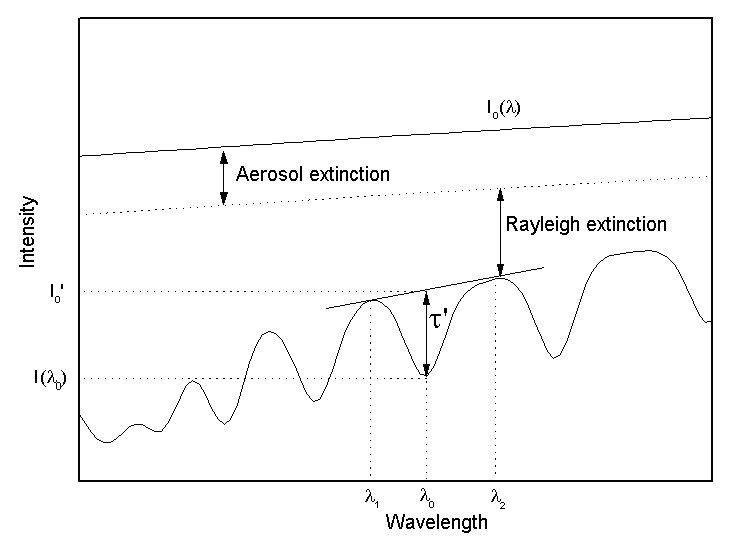
\includegraphics[width=0.8\linewidth]{Bilder/Simon/Bilder_Tung/DOAS_Intensity}
			\caption[Basic idea of the DOAS principle: Light attenuate due to broad band and narrow band effects. Adapted from \citet{kern2009spectroscopic}.]{Basic idea of the DOAS principle: Light attenuate due to broad band and narrow band effects. The broad band extinction is caused by aerosols and Raylight scattering $\left(I_0\rightarrow I^{'}\right)$. The measured intensity $I$ is formed by narrow band effects due to differential absorption structures by trace gases with the optical density $\tau^{'}$. Adapted from \citet{kern2009spectroscopic}}
			\label{fig:doasintensity}
		\end{figure}
	Differential Optical Absorption Spectroscopy (DOAS) was invented in the late 1970s by \citet{perner1979detection}. This section will give an overview about the DOAS technique. More detailed information ca be found in the work of \citet{platt2008differential}\\
	DOAS uses the fact that the broad bands effect do not need to be quantified to determine the column density.
	Therefore it is not necessary to apply \cref{eq:lbe} to real measurements.\\
	\newline
%	\textcolor{red}{Das hier ist ist unter (mathematischer)Debatte. Zumindest bei MAX-DOAS wird das nämlich eigentlich gar nicht gemacht. Der DOAS fit unterteilt gar nicht in Breitband und Schmalband. Die Erklärung hier ist eher eine Illustration wie man sich den DOAS fit vorstellen kann. IM Prinzip ist dieser Abschnitt redundant. Das steht (leider) so nicht im DOAS Buch. Ich bin hier aber voreingenommen. Zu diesem Abschnitt solltest du dir andere Meinungen einholen. ;-) : nicole sat dazu: den Kommentar verstehe ich nicht, falls doch stimmt das geasagte aber nicht }
	Differential Optical Absorption Spectroscopy uses the fact, that absorption can be divided into broad-band parts and narrow-band parts. Broad band parts are effects that only changes weakly with the wavelength,  i.e. scattering and instruments effects have a broad-band structure. 
	The narrow band part includes effects that strongly depends on the wavelength.
	Within the DOAS-Method only narrow-band absorption features of molecules are used to obtain their column densities.
	The absorption cross section of trace gases $j$ have broad-band ($\sigma_b\left(\lambda \right)$) and narrow band ($\sigma{'}\left(\lambda \right)$) features, only the narrow-band structures are used in DOAS.
	\begin{equation}
	\sigma\left(\lambda \right) = \sigma_b\left(\lambda \right) + \sigma{'}\left(\lambda \right)
	\end{equation}

	%
	With this considerations the Beer-Lambert law \cref{eq:lbe} can be rewritten
	dividing the exponential part into a narrow-band part and a broad-band part:

	\begin{align}
	I\left(\lambda,L\right) = &\overbrace{I_{0}\left(\lambda\right)\cdot exp\left(-\int^{L}_{0}\sum_{j}\sigma_{b,j}\left(\lambda,p,T\right)\cdot c_{j}\left(l\right)+\epsilon_R\left(\lambda,l\right)+\epsilon_{M}\left(\lambda,l\right)dl\right)}^{=I^{'}_0\left(\lambda\right)} \cdot \nonumber \\
	&exp\left(-\int^{L}_{0}\sum_{j}\sigma_{j}^{'}\left(\lambda,p,T\right)\cdot c_{j}\left(l\right)dl\right)
	\label{eq:bb}
	\end{align}	
		%
	The so defined $I^{'}_0\left(\lambda\right)$ differs from $I_0\left(\lambda\right)$ only by broad band effects. In this context the dependency of the absorption cross section on the temperature and the pressure can be neglected. With $I^{'}_0\left(\lambda\right)$ a differential optical density $\tau^{'}$ can be defined:
	\begin{equation}
	\tau^{'} = ln\left(\frac{I^{'}_0\left(\lambda\right)}{I\left(\lambda\right)}\right) = \int_{0}^{L} \sum_{j} \sigma^{'}_{j}\left(\lambda\right) \cdot c_{j}\left(l\right)dl = \sum_{j}\sigma^{'}_{j}\left(\lambda\right)\cdot S_{j}
	\label{eq:taustrich}
	\end{equation}
	
	The optical density can now be calculated by using the difference of the column density $S_{M}$ in the measurement spectrum to the column density $S_{R}$ of a reference spectrum. From \cref{eq:bb} it is known:	
	\begin{equation}
	I_{M,R} = I^{'}_{0}\cdot exp\left(-S_{P,R}\cdot\sigma\left(\lambda\right)\right)\footnote{M: Measuremtn, R: Reference}
	\label{eq:smr}
	\end{equation}
	
	In general the obtained column density $S_{M}$ is called differential slant column density: "dSCD". If the reference spectrum does not contain the trace gas of interest (is not contaminated with trace gases) that means $S_{R} = 0$, $S_{M}$ is called the slant column	density (SCD). 
	With \cref{eq:smr} the optical density can be derived by:
	\begin{equation}
	\tau\left(\lambda\right) = -ln\left(\frac{I_{M}}{I_{R}}\right) = \sigma\left(\lambda\right)\cdot\left(S_{M}-S_{R}\right)
	\end{equation}
	%
	
	
	\subsection{Technical implementation of the DOAS approach}
	The theory explained above only describes the ideally situation. In real measurements more problems occur due to instrument limitations inelastic scattering causing the Ring effect and due to impacts of external parameters like temperature.\\
	In the following a short overview about these problems and their consequences for our retrieval is given. Further information can be found in \citet{lubcke2014optical}.\\
	\subsubsection*{Optical and spectral resolution of the spectrometer}
	The resolution of the spectrometer is finite, thus, the detector receives a spectrum $I^{*}\left(\lambda\right)$ which can be retrieved with a convolution of the incident spectrum $I\left(\lambda\right)$ with the instrument function H$\left(\lambda\right)$:
	\begin{equation}
	I^{*}\left(\lambda\right) = I\left(\lambda\right)*H\left(\lambda\right)=\int I\left(\lambda-\lambda{'}\right)\cdot H\left(\lambda-\lambda{'}\right)d\lambda{'}
	\end{equation} 
	For the evaluation all $\sigma_{j}$  of the trace gases of interest need to have the same spectral resolution as the instrument used for recording the spectra. In this work I will use high resolution cross sections and convolute them with the instrument function H:
	\begin{equation}
	\sigma{*}\left(\lambda\right) = \sigma\left(\lambda\right)*H\left(\lambda\right)
	\end{equation}
%	\textcolor{red}{bessere Darstellung zu $\sigma{*}$}
	The instrument function H can be approximated by using a the spectral lines of an mercury lamp since the width of those lines is only a few pm, they could be treated as delta peaks when comparing it to the resolution of the spectrometers.
	
	\subsubsection*{Effects of the detector}
	The detector only has discrete pixels, therefore a wavelength interval is mapped to a pixel $i$.
	
	\begin{equation}
	I^{'}\left(i\right) = \int_{\lambda(i)}^{\lambda(i+1)}I^{*}\left(\lambda{'}d\right)d\lambda{'}
	\end{equation}
	For the retrieval the relationship between the detector channels and the wavelength of the spectrum need to be known.
	The wavelength to pixel mapping (WPM) for a detector with q channels can be calculated as:

	\begin{eqnarray}
	\lambda(i) = \sum_{k=0}^{q-1}\gamma_{k}\cdot i^{k}
	\end{eqnarray}
	Hereby, is $\gamma_{0}$ a shift of the spectrum and $\gamma_{1}$ is a squeeze (respectively stretch) of the spectrum.
	The wavelength to pixel mapping can be discovered by using a mercury lamp again and compare pixel-position with the well known wavelength of the individual HG-lines of the mercury lamp.\\
	The wavelength to pixel mapping depends on the instrument temperature as well as on the ambient pressure \citep{lubcke2014bro}.
	\subsubsection*{Ring effect}
	As mentioned above inelastic scattering causes the Ring effect (named after Grainger and Ring, 1962).
	The Ring effect is observable through a filling of the Fraunehofer lines in spectra of scattered solar radiation, (e.g. if the sunlight travels through the earth atmosphere). When compared to direct sunlight measurements (e.g. outside of the earth atmosphere).
	(\citet{bussemer1993ring},\citet{solomon1987interpretation}) identified rotational Raman scattering mainly of
	\ce{O2} and \ce{N2} in the atmosphere as the origin of the Ring effect.
	\citet{solomon1987interpretation} suggested to treat the Ring effect as a pseudo-absorber. 

%%

	\section{Evaluation routine}
	The fitting routine used for this thesis is based on the DOASIS software \citep{kraus2006doasis}. 
	The equations of the DOAS retrieval of this work are slightly different from \Cref{eq:taustrich} and therefore described in the following.
	\Cref{eq:lbe} can be rewritten as:
	\begin{align}
	ln\left(I\left(\lambda, L\right)\right) = &ln\left(I_0 \right) + P \left(\lambda\right) -	\int_{0}^{L}\sum_{j}\sigma_j \left(\lambda, p, T \right) \cdot c_j \left(l\right)dl \nonumber \\
	= &ln\left(I_0 \right) + P \left(\lambda\right)-
	\sum_{j}\sigma_j \left(\lambda, p, T \right) \cdot S_j
	\label{eq:lben}
	\end{align}
	%
	The polynomial $ P \left(\lambda\right)$ accounts for all broad-band effects which approximates the scattering effects of the atmosphere as well as broad band absorptions.
	
	The task of the DOAS retrieval is to find a model function $F \left(\lambda\right)$ that minimizes $\chi^2$:
	\begin{equation}
	\chi^2 = \sum_{i=\lambda_1}^{\lambda_2}\left(ln(I(i))-F(i)\right)^2
	\label{eq:Chi}
	\end{equation}
	While $F\left(\lambda\right)$ can be expressed on the basis of \Cref{eq:lben}:
	\begin{equation}
	F\left(\lambda\right) = ln\left(I_0 \right) + P \left(\lambda\right)-
	\sum_{j}\sigma_j \left(\lambda\right) \cdot S_j
	\label{eq:F}
	\end{equation}
	The DOAS fitting routine uses a combination of a standard least-squares fit and a Levenberg-Marquard algorithm to minimize $\chi^2$\\
	\\
	Prior to the DOAS fitting. the spectra need to be calibrated, this done by using a wavelength to pixel mapping function (WMP) developed by \citet{lehmann2011improving}. The WMP uses a solar atlas spectrum that is concolced with the Hg line of the single instruments, hereby am initial calibration based on the Hg lines is given as a first parameter. The calibration is done by fitting the Fraunhofer lines of the recorded spectrum on the convolved Solar Atlas spectrum. The Rayleigh scattering is considered by adding a Ring spectrum as well as a wavelength dependent Ring spectrum (proportional to $\lambda^4$) \citep{wagner2009three}. Mie scattering and broadband absorption structures were accounted due to adding a third order polynomial to the retrieval well as an offset polynomial to correct for stray-light influence \citep{lubcke2014bro}.\\
	The \ce{SO2} evaluation is performed for a wavelength range between 314.8~nm and 328~nm. Including a \ce{SO2} absorption cross section recorded at a temperature of 298K \citep{vandaele2009fourier} and a  \ce{O3} absorption cross section recorded at 221K \citep{burrows1999atmospheric}.\\
	The \ce{BrO}  evaluation is performed for a wavelength range between 330.6~nm and 352.7~nm (found by \citet{vogel2011volcanic}). The sum in \Cref{eq:F} includes for the BrO evaluation the following absorption cross sections:
	\ce{BrO}  at 298K \citep{fleischmann2004new}, the \ce{SO2} and  \ce{O3} absorption cross sections described above, \ce{O4} \citep{hermans2003absorption},  \ce{NO2} at 298K \citep{vandaele1998measurements} and  \ce{CH2O} at 298K \citep{meller2000temperature}.\\
	%
	The choice of the wavelength range as well as the considered trace gases used in the fits is based on studies on the optimal evaluation wavelength range in a combination of real measurement data and theoretical studies \\
	%
	The choice of the wavelength range as well as the considered tracfor BrO and \ce{SO2}, made by \citet{vogel2011volcanic}.\\
	The spectra of the trace gases were convoluted by using the 334.15 nm line of a mercury lamp.\\
	A further effect influencing the evaluation is the $I_{0}$ effect, in order to account for the I0-effect \citep{platt2008differential} an iterative approach was used. Further informations can be found at (Wagner et al., 2002), \cite{lubcke2014bro},\cite{vogel2011volcanic}).
	To further correct for small inaccuracies of the WMP, the FRS and both Ring spectra as one set, and all trace gases absorption cross sections as another set, are allowed to be shifted, and first order squeezed against the measurement spectrum.\\
	%
	NOVAC provides spectral data for roughly 50 different elevation angles. For the DOAS evaluation a reference and a measurement spectrum is needed. Obtaining the complete amount of volcanic gases is only possible in the case of the availability of references which is free of the volcanic gases of interest (this will be discussed more detailed in \Cref{Chap:Cont}). The column density of  \ce{BrO}  and \ce{SO2} of the measurement spectrum relatively to the reference spectrum can be calculated \Cref{eq:Chi} and \ref{eq:F}. \\
	\\
	\begin{figure}
		\subfigure[]{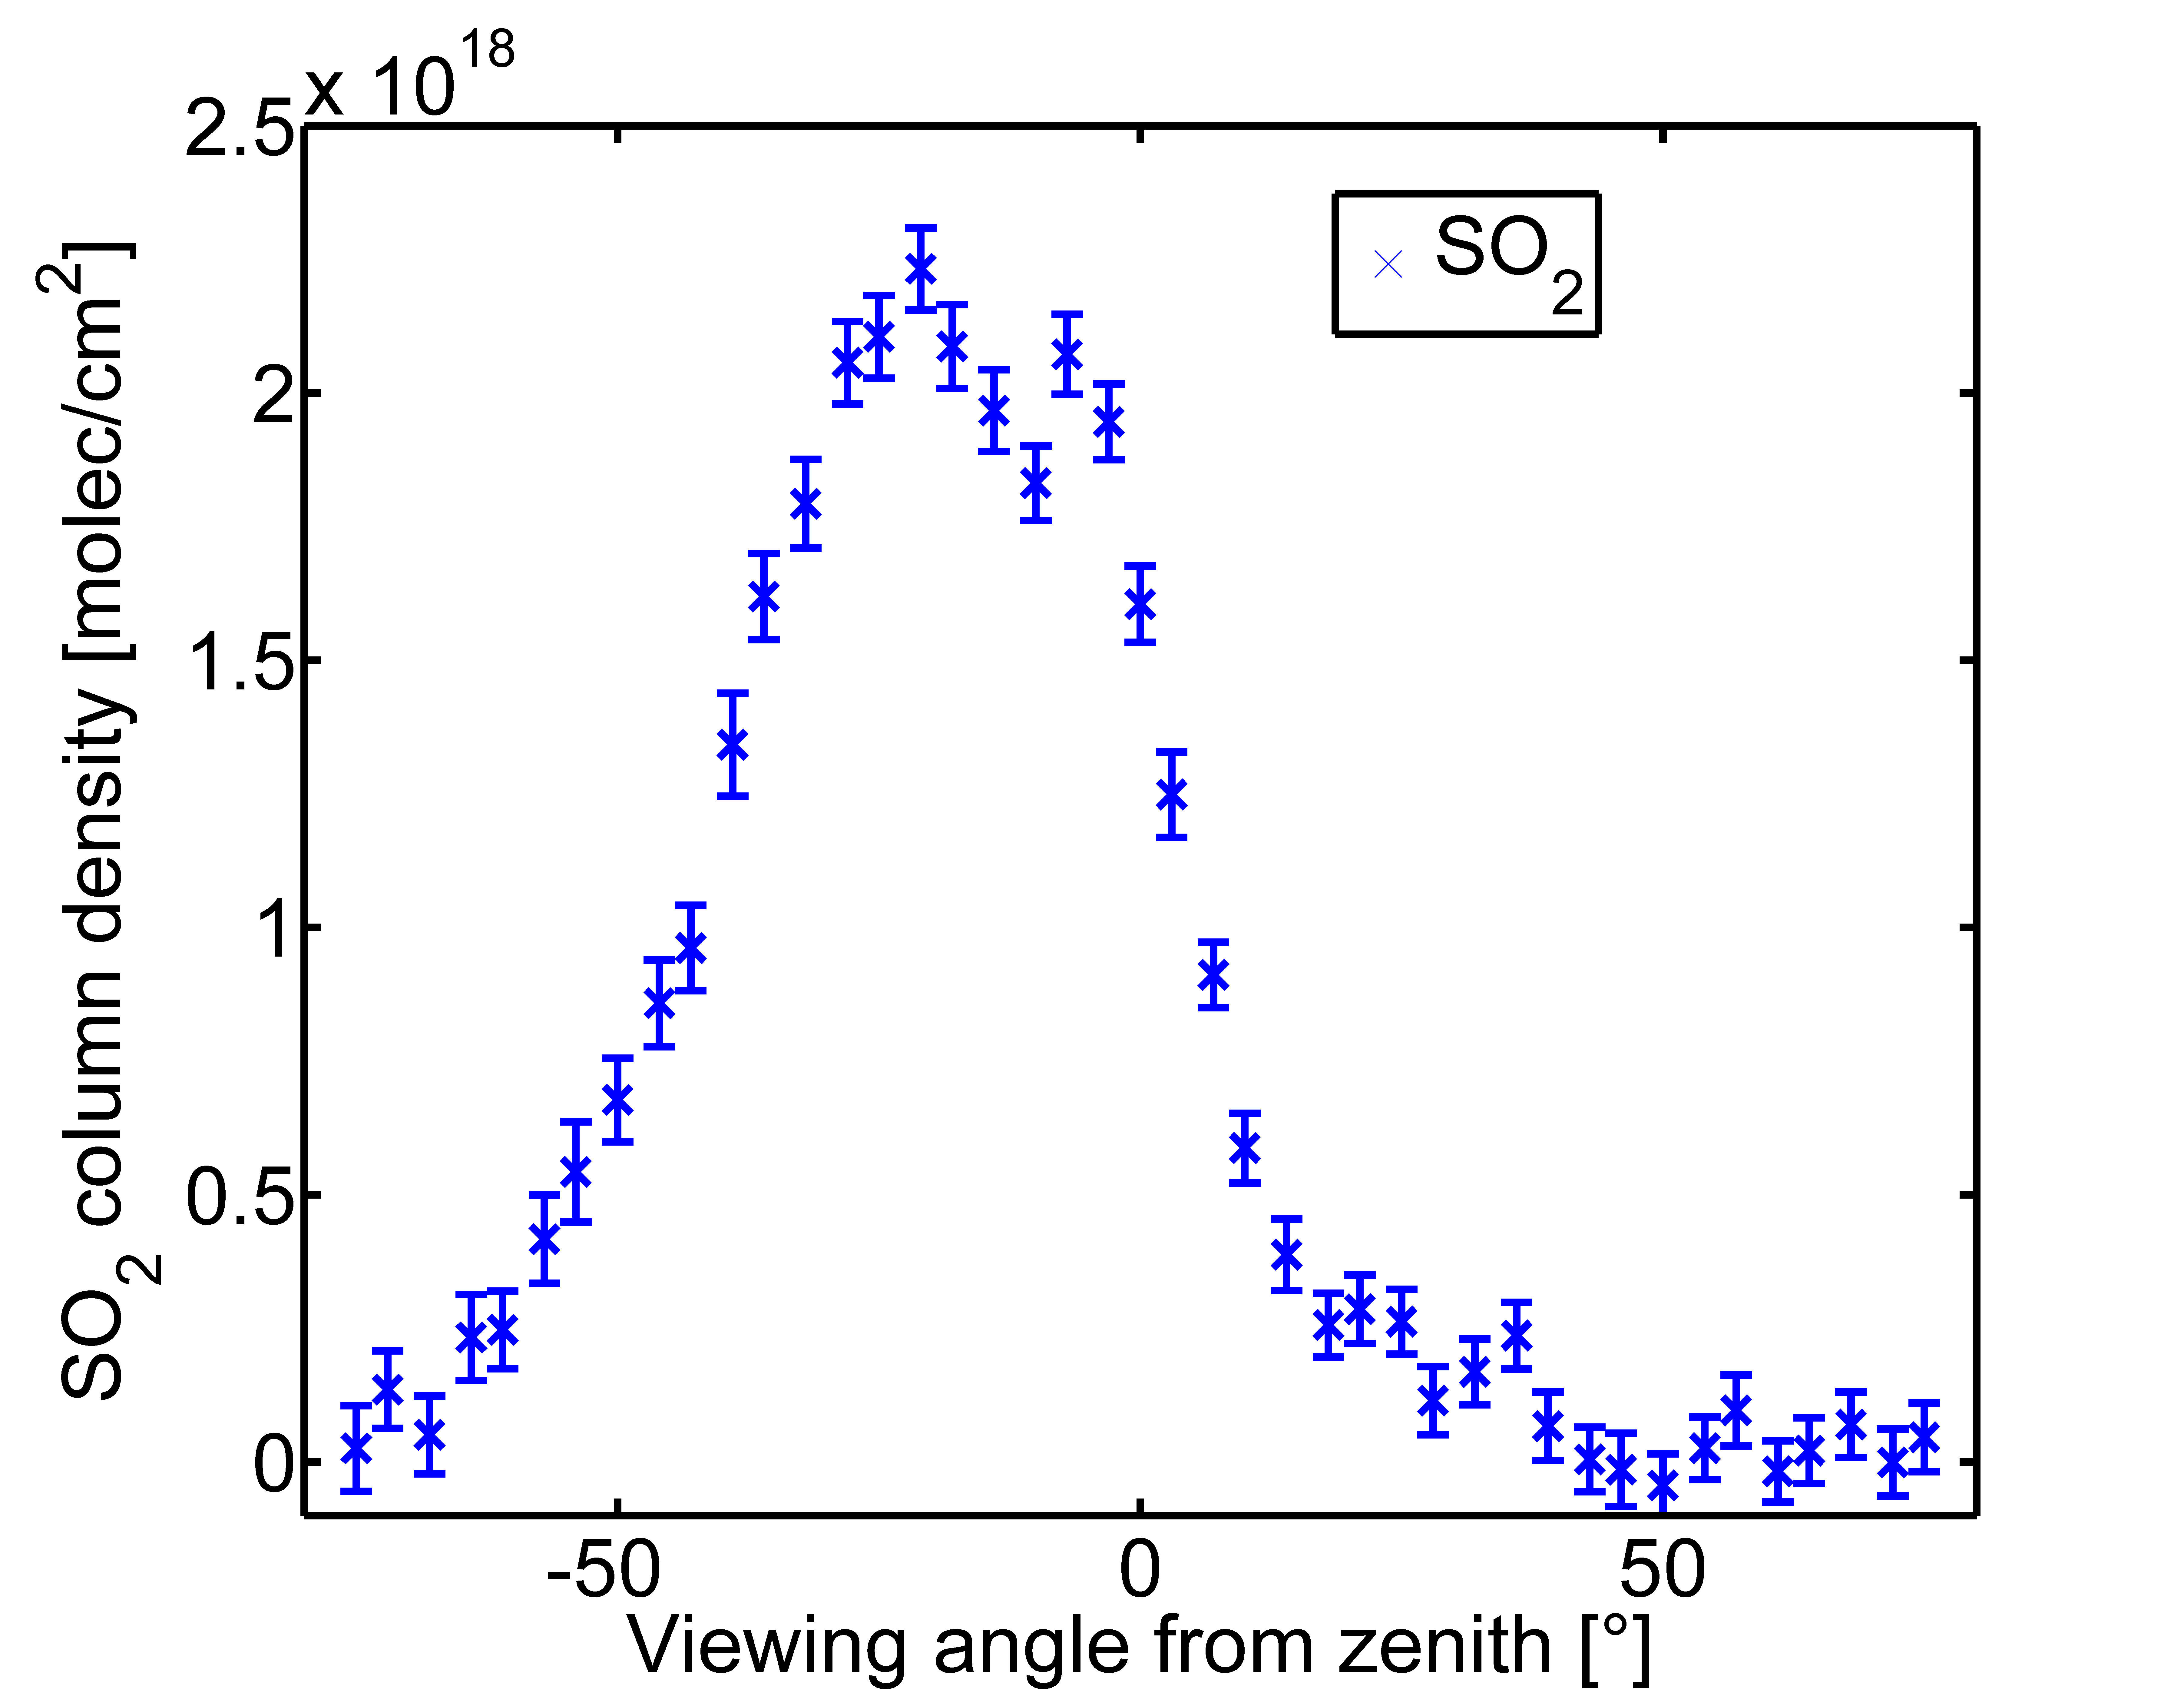
\includegraphics[width=0.51\textwidth]{Bilder/Simon/Bilder_Tung/SO2_Scan_0}}
		\subfigure[]{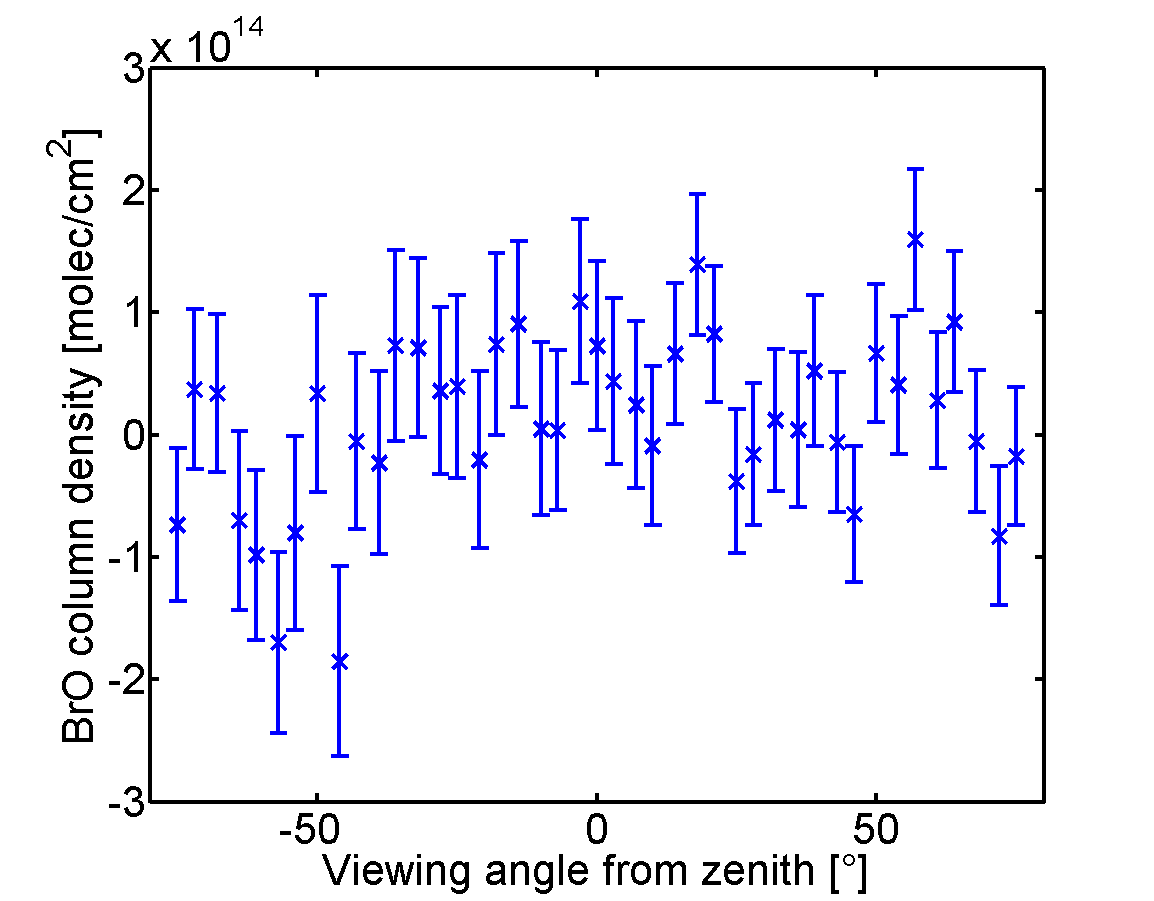
\includegraphics[width=0.51\textwidth]{Bilder/Simon/Bilder_Tung/BrO_Scan}}
		\caption[(a) \ce{SO2} SCD as a function of the elevation angle with error bars computed by the DOASIS fitting routin. (b) \ce{BrO} SCD as a function of the elevation angle computed by the DOASIS fitting routine.  Taken from \cite{WarnachSimon}]{(a) \ce{SO2} SCD as a function of the elevation angle with error bars computed by the DOASIS fitting routin. (b) \ce{BrO} SCD as a function of the elevation angle with fit error bars computed by the DOASIS fitting routine.  Taken from \cite{WarnachSimon}}
		\label{fig:plumeref}
	\end{figure}

	
	\section{Conventional evaluation routine\label{Chap:evalroutine}}
	

%% NOVAC
%% =============
%%
This chapter outlines the algorithm which is used for the evaluation of the spectroscopic data recorded in NOVAC. 
The problem of contamination of the reference is explained and possible solutions are presented.

\section{Conventional evaluation routine}
The fitting routine used for this thesis is based on the DOASIS software \citep{kraus2006doasis}. 
The equations of the DOAS retrieval of this work are slightly different from \Cref{eq:taustrich} and therefore described in the following.
\Cref{eq:lbe} can be rewritten as:
\begin{align}
ln\left(I\left(\lambda, L\right)\right) = &ln\left(I_0 \right) + P \left(\lambda\right) -	\int_{0}^{L}\sum_{j}\sigma_j \left(\lambda, p, T \right) \cdot c_j \left(l\right)dl \nonumber \\
= &ln\left(I_0 \right) + P \left(\lambda\right)-
\sum_{j}\sigma_j \left(\lambda, p, T \right) \cdot S_j
\label{eq:lben}
\end{align}
%
The polynomial $ P \left(\lambda\right)$ accounts for all broad-band effects which approximates the scattering effects of the atmosphere as well as broad band absorptions.

The task of the DOAS retrieval is to find a model function $F \left(\lambda\right)$ that minimizes $\chi^2$:
\begin{equation}
\chi^2 = \sum_{i=\lambda_1}^{\lambda_2}\left(ln(I(i))-F(i)\right)^2
\label{eq:Chi}
\end{equation}
While $F\left(\lambda\right)$ can be expressed on the basis of \Cref{eq:lben}:
\begin{equation}
F\left(\lambda\right) = ln\left(I_0 \right) + P \left(\lambda\right)-
\sum_{j}\sigma_j \left(\lambda\right) \cdot S_j
\label{eq:F}
\end{equation}
The DOAS fitting routine uses a combination of a standard least-squares fit and a Levenberg-Marquard algorithm to minimize $\chi^2$\\
\\
Prior to the DOAS fitting. the spectra need to be calibrated, this done by using a wavelength to pixel mapping function (WMP) developed by \citet{lehman 2014}. The WMP uses a solar atlas spectrum that is concolced with the Hg line of the single instruments, hereby am initial calibration based on the Hg lines is given as a first parameter. The calibration is done by fitting the Fraunhofer lines of the recorded spectrum on the convolved Solar Atlas spectrum. The Rayleigh scattering is considered by adding a Ring spectrum as well as a wavelength dependent Ring spectrum (proportional to $\lambda^4$) \citep{wagner2009}. Mie scattering and broadband absorption structures were accounted due to adding a third order polynomial to the retrieval well as an offset polynomial to correct for stray-light influence \citep{lubcke2014bro}.\\
The \ce{SO2} evaluation is performed for a wavelength range between 314.8~nm and 328~nm. Including a \ce{SO2} absorption cross section recorded at a temperature of 298K \citep{vandaele2009fourier} and a  \ce{O3} absorption cross section recorded at 221K \citep{burrows1999atmospheric}.\\
The \ce{BrO}  evaluation is performed for a wavelength range between 330.6~nm and 352.7~nm (found by \citet{vogel2011volcanic}). The sum in \Cref{eq:F} includes for the BrO evaluation the following absorption cross sections:
\ce{BrO}  at 298K \citep{fleischmann2004new}, the \ce{SO2} and  \ce{O3} absorption cross sections described above, \ce{O4} \citep{hermans2003absorption},  \ce{NO2} at 298K \citep{vandaele1998measurements} and  \ce{CH2O} at 298K \citep{meller2000temperature}.\\
%
The choice of the wavelength range as well as the considered trace gases used in the fits is based on studies on the optimal evaluation wavelength range in a combination of real measurement data and theoretical studies for BrO and SO2, made by \citet{vogel2011volcanic}.\\
The spectra of the trace gases were convoluted by using the 334.15 nm line of a mercury lamp.\\
A further effect influencing the evaluation is the $I_{0}$ effect, in order to account for the I0-effect \citep{platt2008differential} an
iterative approach was used. Further informations can be found at (Wagner et al., 2002), \cite{lubcke2014bro},\cite{vogel2011volcanic}).
To further correct for small inaccuracies of the WMP, the FRS and both Ring spectra as one set, and all trace gases absorption cross sections as another set, are allowed to be shifted, and first order squeezed against the measurement spectrum.\\
%
NOVAC provides spectral data for roughly 50 different elevation angles. For the DOAS evaluation a reference and a measurement spectrum is needed. Obtaining the complete amount of volcanic gases is only possible in the case of the availability of references which are free of volcanic gases of interest(this will be discussed more detailed in \Cref{Chap:Cont}). The column density of  \ce{BrO}  and \ce{SO2} of the measurement spectrum relatively to the reference spectrum can be calculated \Cref{eq:Chi} and \ref{eq:F}. \\
\\
\begin{figure}
	\subfigure[]{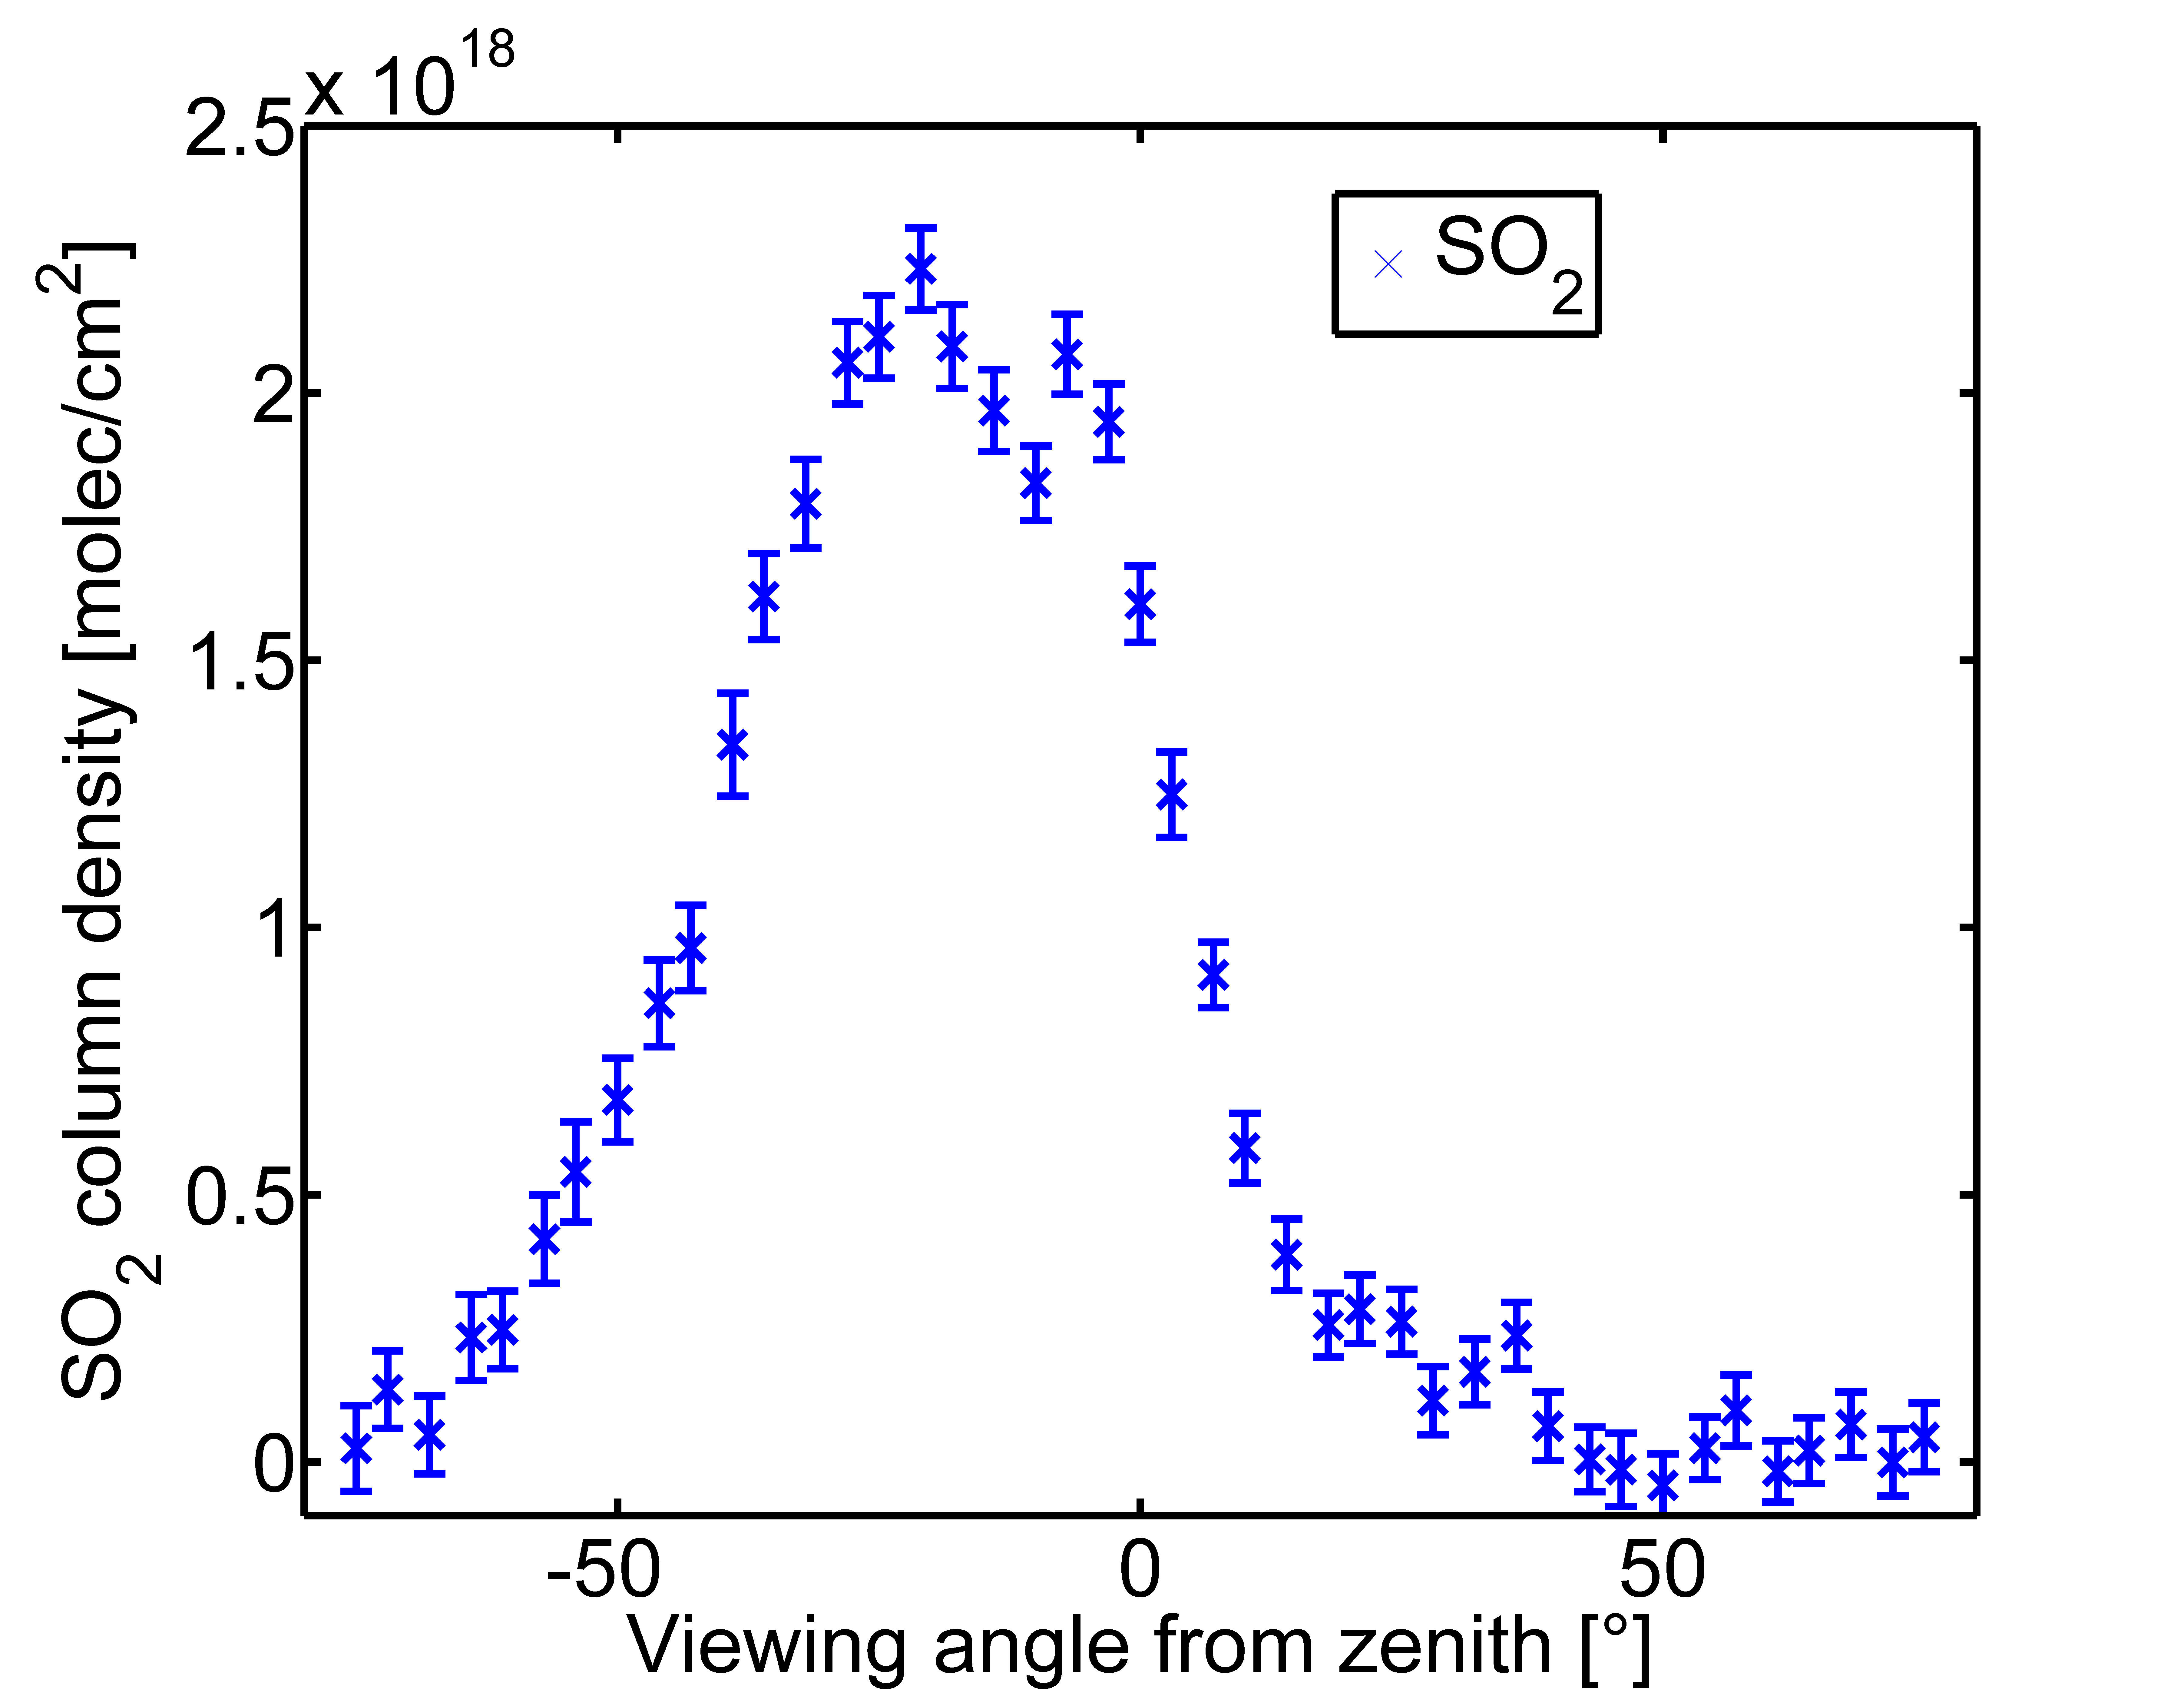
\includegraphics[width=0.51\textwidth]{Bilder/Simon/Bilder_Tung/SO2_Scan_0}}
	\subfigure[]{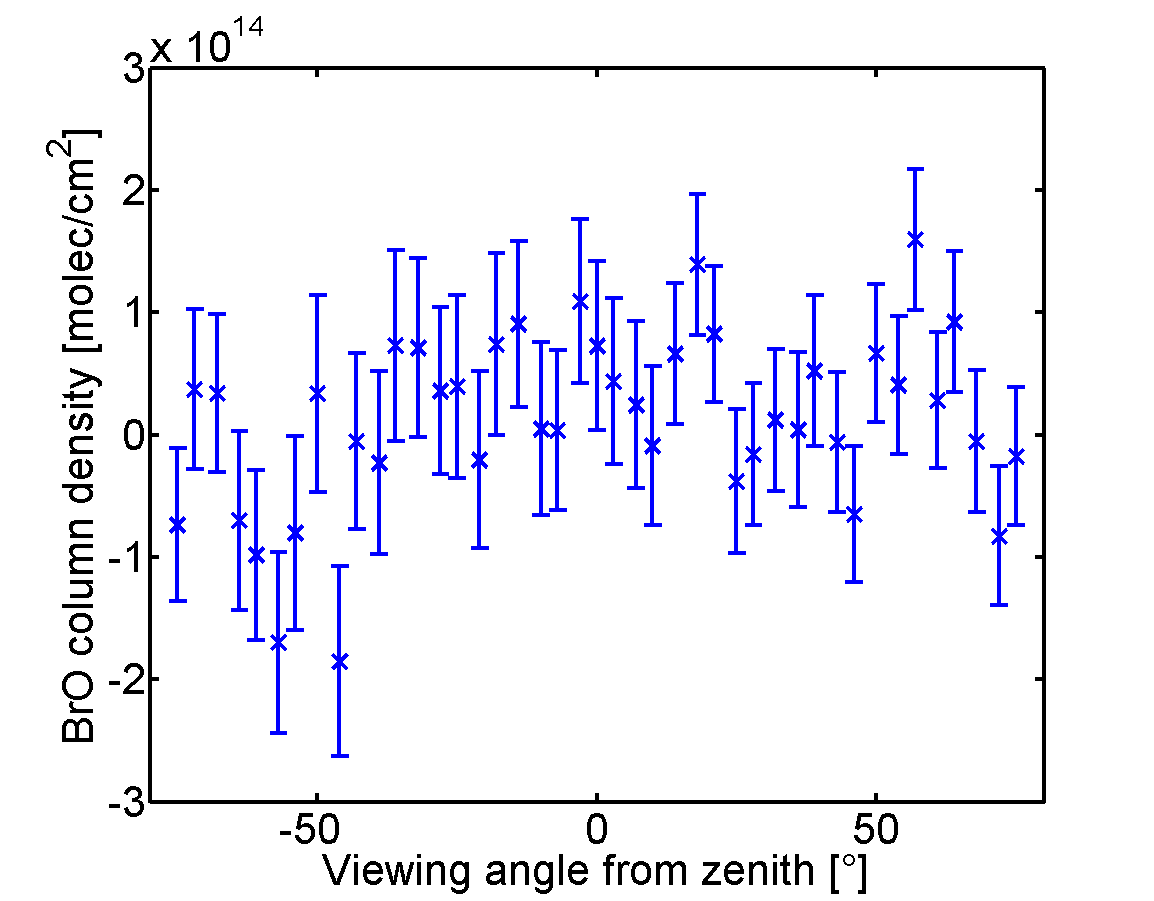
\includegraphics[width=0.51\textwidth]{Bilder/Simon/Bilder_Tung/BrO_Scan}}
	\caption{(a) \ce{SO2} SCD as a function of the elevation angle with error bars computed by the DOASIS fitting routin. (b) \ce{BrO} SCD as a function of the elevation angle with error bars computed by the DOASIS fitting routine.  Taken from \cite{WarnachSimon}}
	\label{fig:plumeref}
\end{figure}
%
In the following we describe the technical implementation of the DOAS approach using the data of NOVAC instruments:\\
%
The first step is to correct each spectrum of the scan for dark current and offset using the dark spectrum.
The next task is to locate the spectra in and outside of the volcanic plume.
First a "pre-reference" (the spectrum recorded at an elevation angle of  0$^{\circ} $) is used to perform the evaluation of the scan spectra recorded at every elevation angle.
For every spectrum of the scan the \ce{SO2} differential slant column density (dSCD) with respect to the pre-reference is calculated using \Cref{eq:F} by the DOASIS fit routine.

The result is \ce{SO2} dSCDs as a function of the elevation angle. This way the elevation angle corresponding to the maximum and the minimum of the \ce{SO2} column density can be determined. The location of the \ce{SO2} maximum defines the location of the plume. The assumption is that the minimum of the \ce{SO2} curve corresponds to a region outside of the plume which is true in most cases. The background \ce{SO2} amount in the earth atmosphere around Tungurahua is usually negligible (see  \Cref{chap:so2}) so we take it as a region of zero \ce{SO2}. \\
We use a gauss fit of the \ce{SO2}-elevation-angle-curve to define the plume region.
%
\begin{figure}
	\centering
	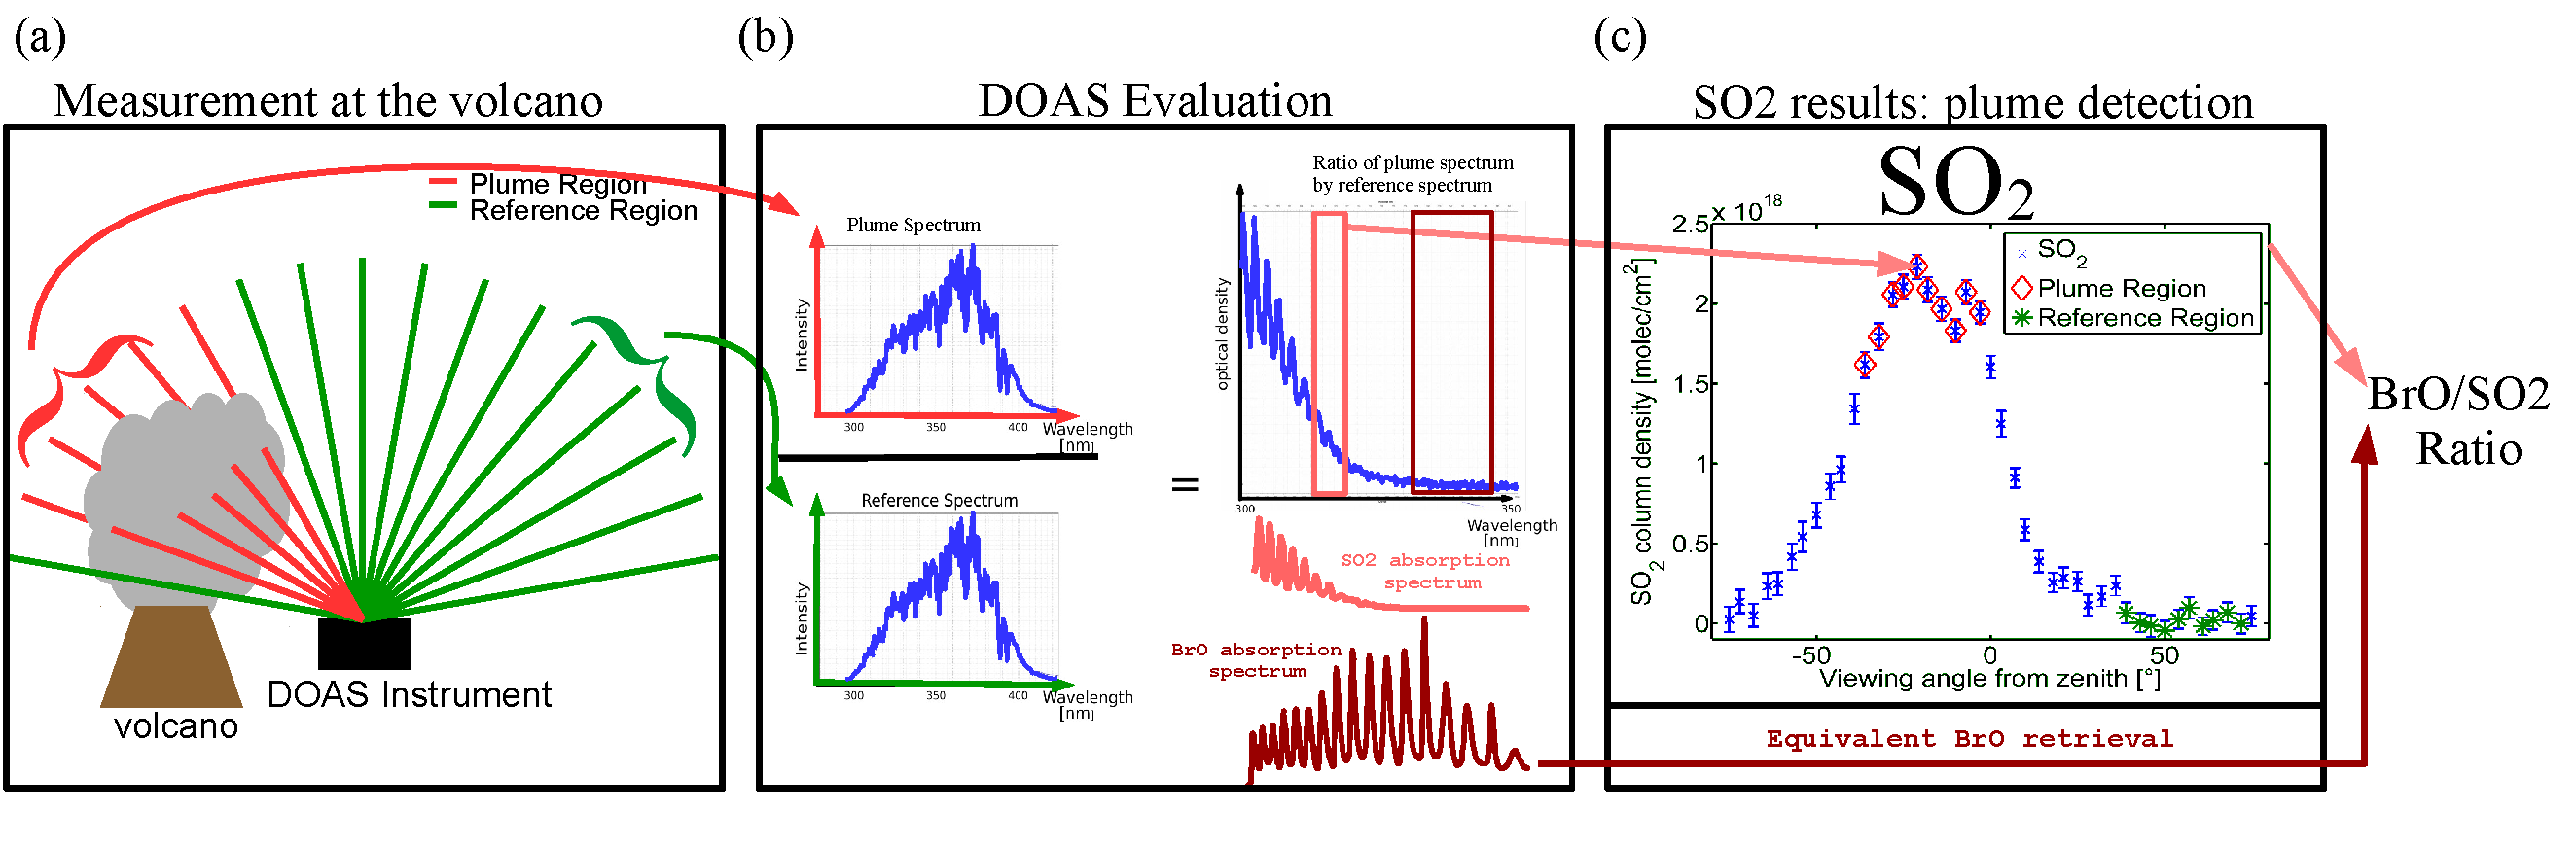
\includegraphics[width=1\linewidth]{Bilder/NOVAC_Eval}
	\caption{NOVAC Evaluation: (a) Measurement at the volcano (b) Evaluation of the spectral data with the DOAS routine using the absorption cross sections of \ce{BrO}  and \ce{SO2}. (c) Finding the location of the plume and reference (taken from \cite{WarnachSimon}) (d) Computation of the ratios BrO/\ce{SO2}}
	\label{fig:NOVAC_Eval}
\end{figure}
The sum over all plume spectra is taken, which are in the elevation angle interval of the gauss peak plus minus one sigma, to increase the photon statistic and to reduce the residuum. If the gauss curve is too wide, what this means in specific is that more then 10 spectra are added within the gauss evaluation, The running mean is calculated and the 10 spectra with the highest \ce{SO2} amount are used for the retrieval. As reference we use the sum of the 10 spectra with the lowest \ce{SO2} amount.\\
The absolute slant column densities (SCD's) of \ce{BrO}  and \ce{SO2} can now be calculated with the previously defined reference and plume spectrum.
In \Cref{fig:plumeref} (a) an example \ce{SO2} SCD as a function of the elevation angle is shown. The \ce{SO2} curve has a maximum at the position of the plume at an elevation angle of approximately $-30^{\circ}$ to $0^{\circ}$  and a reference region at an elevation angle of $40^{\circ}$ to $70^{\circ}$. \Cref{fig:plumeref} (b)  illustrates that  extrema of the \ce{BrO}  curve are not as distinct as it is the case for the \ce{SO2} curve.\\
Since the \ce{BrO} column density is much lower than the \ce{SO2} column density, and just lies slightly above the detection limit, the plume is hard to detect using the \ce{BrO} column density as it is shown in fig. \ref{fig:plumeref} (b). 
Therefore we evaluate BrO only in the plume location determined by using \ce{SO2}.\\
In a further step multiple reference and plume spectra of successive measurements are added to further increase the fit quality.
\Cref{fig:NOVAC_Eval} visualizes the different steps described above in the retrieval of the BrO/\ce{SO2} ratios.\\
\Cref{fig:algorithm} (b) shows the routine of adding multiple spectra of consecutive measuring times. In the following the spectra resulting from the multi adding technique will be referred to as "Multi Add Spectra". The algorithm for co-adding is visualized in \Cref{fig:algorithm} (b) was invented by \citet{vogel2011volcanic} and \citet{lubcke2014bro}.\\
%
Taking the \ce{BrO}/\ce{SO2} molar ratios if the column densities are close to zero yields unpredictable and unrealistic results. Thus, spectra measured in a thin volcano plume need to be excluded.
This could be achieved by setting a \ce{BrO} or/and an \ce{SO2} threshold. A reasonable \ce{BrO} threshold needs to be at least in the order of the DOAS fit error. However this could lead to elevated \ce{BrO}/\ce{SO2} ratios, since the \ce{BrO} error is often close to the detection limit. Thus, all low \ce{BrO} column densities are excluded from the evaluation  \citep{lubcke2014bro}, as an effect the ratios are systematic to high.
%
\begin{figure}
	\subfigure[ ]{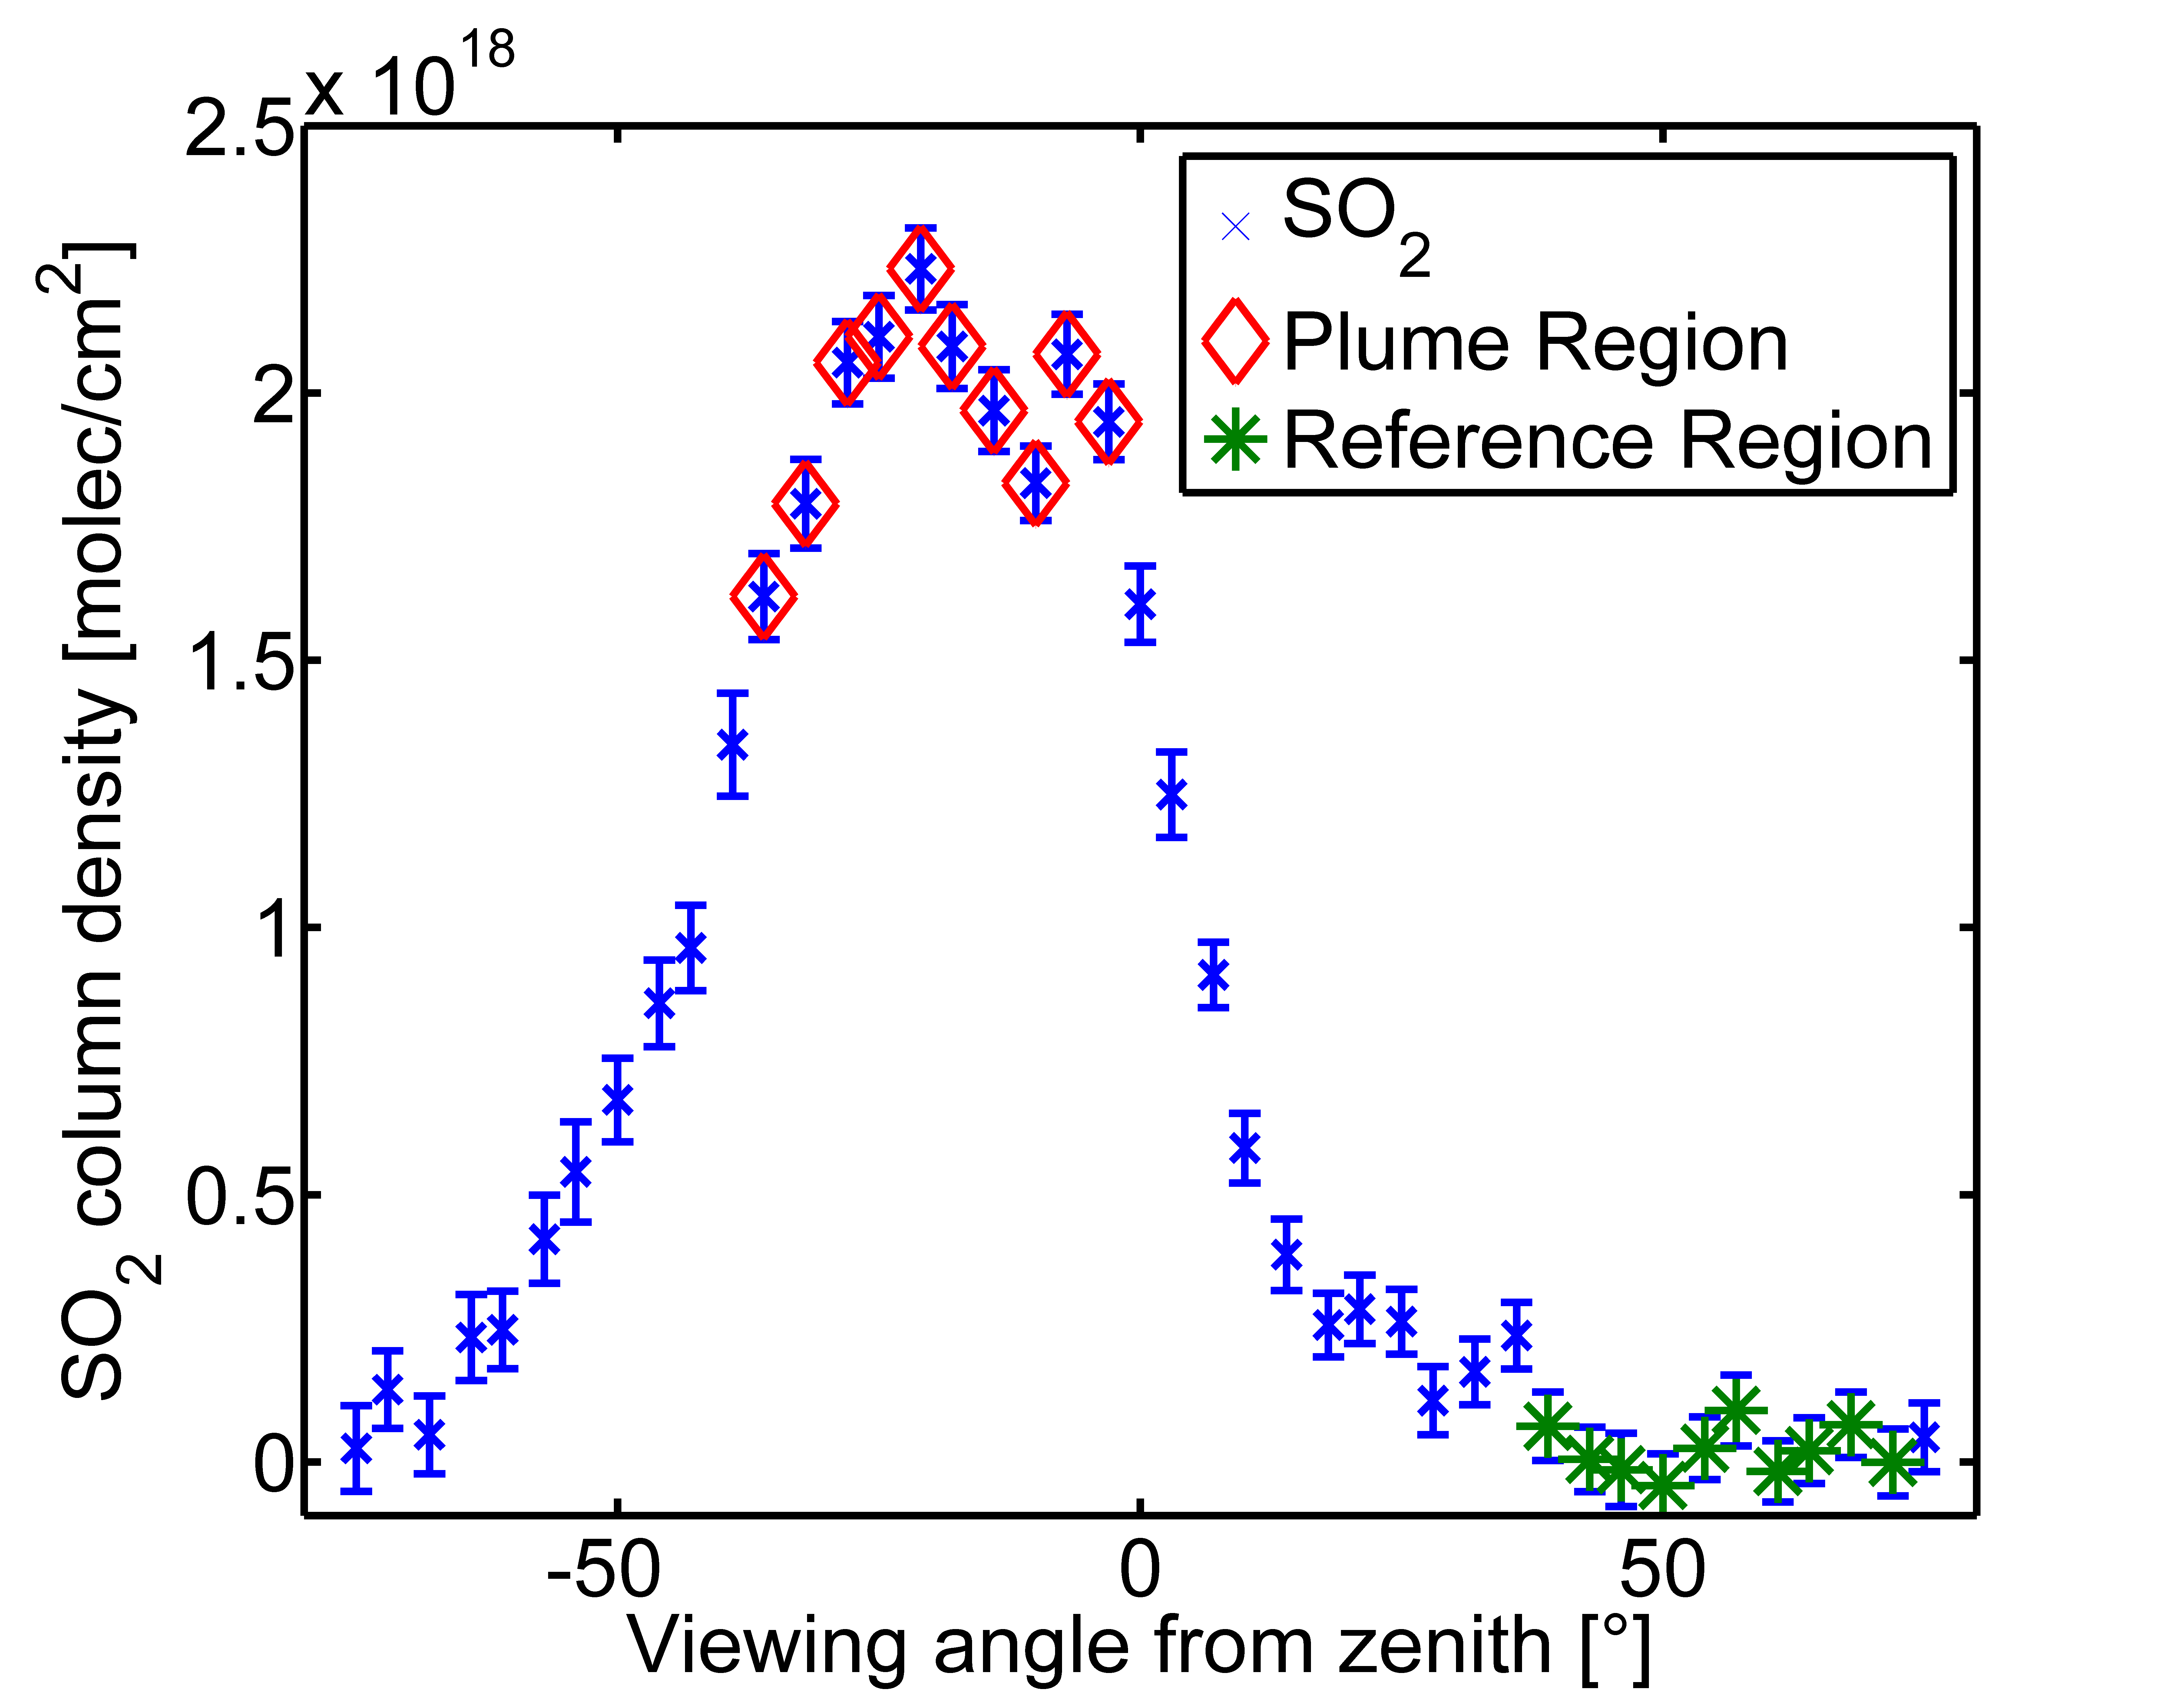
\includegraphics[width=0.53\textwidth]{Bilder/Simon/Bilder_Tung/SO2_Scan}}
	\subfigure[ ]{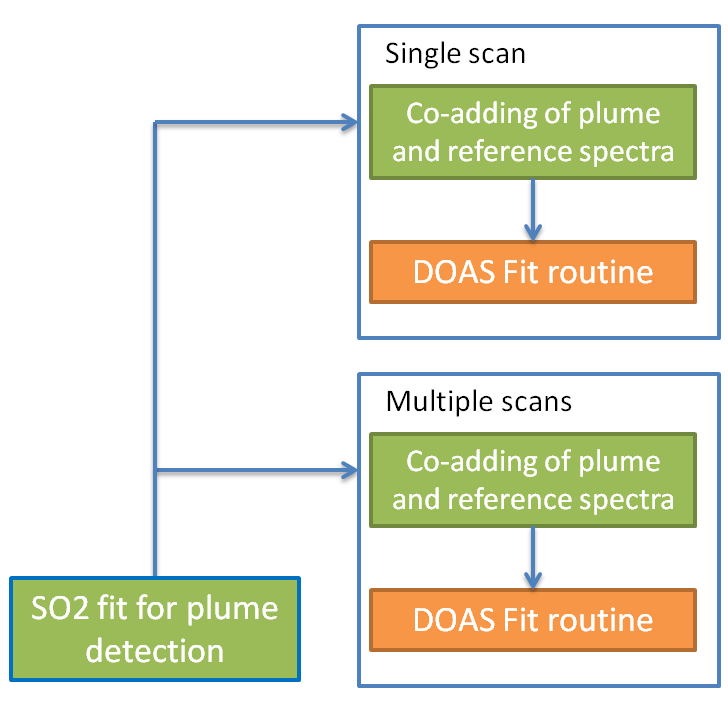
\includegraphics[width=0.47\textwidth]{Bilder/Simon/Bilder_Tung/Algorithm}}
	\caption{(a) \ce{SO2} SCD as a function of the elevation angle. The co-added plume region is marked with red diamonds, and the co added reference region with green stars. From \cite{WarnachSimon}. (b) Flow chart of the \ce{BrO}  and \ce{SO2} evaluation. From \cite{lubcke2014optical}.}
	\label{fig:algorithm}
\end{figure}
The other possibility is to set an \ce{SO2} threshold. In this thesis an \ce{SO2} threshold (plume limit) of $7\cdot 10^{17} \frac{molec}{cm^2}$ is used for the selection of spectra for the evaluation of the \ce{BrO}/\ce{SO2} ratio. $7\cdot 10^{17} \frac{molec}{cm^2}$ is a high threshold for the column density. However, this approach assures that only strongly significant gas amounts are accounted \citep{lubcke2014bro}. Choosing the \ce{SO2} threshold in this way leads to consistent observations for strong degassing, but low degassing events are rather excluded in the evaluation.\\
\textcolor{red}{Ich würde hier noch erwähnen für welche Ratios wir mit diesem Plume Limit sensitiv sind (siehe Appendix in Dinger et al, 2018).}\\
Increasing a plume limit leads to a decrease of usable data. The ratio of usable  data as a function of the plume limit is shown in \Cref{fig:percentageminso2}. An exponential decrease of data can be observed. The plot is based on the data of Tungurahua. Plume limits below 7$\cdot10^{17}$ are shaded in yellow. A plume limit of 7$\cdot10^{17}$ leads to a ratio of usable data of approximately 10\%.
\begin{figure}
	\centering
	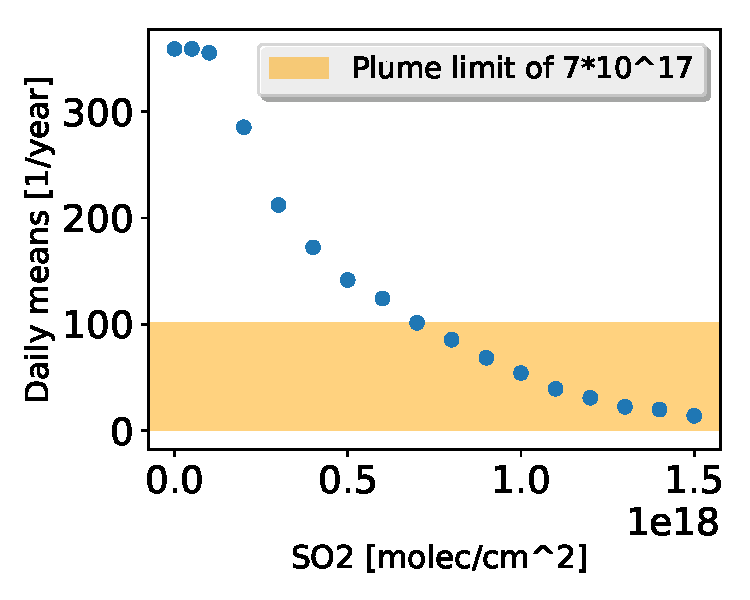
\includegraphics[width=0.7\linewidth]{Bilder/percentage_minSO2}
	\caption{The decrease of the amount of data above the plume limit as a function of the plume limit. The plume limits below the actual plume limit of 7$\cdot10^{17}$ are marked with a yellow shade.\textcolor{red}{noch dazu:In Prozent sieht das in der Tat schrecklich aus, relevant für eine Zeitreihenanalyse ist aber eher die (absolute) Anzahl der Tage mit (Multi-Scan-)Daten. Vielleicht als zweites Bild daneben?! }}
	\label{fig:percentageminso2}
\end{figure}

\section{Contamination problem\label{Chap:Cont}}
The conventional Evaluation is based on the assumption, that the reference is free of volcanic gases. This assumption was checked by using a volcanic gas free a high resolution solar atlas spectrum (see below) to evaluate the reference \cite{lubcke2014}; \cite{salerno2009novel}. In some reference spectra an amount of \ce{SO2}  different from zero is found. Thus we can conclude, that there are some references which contain a non-negligible amount of volcanic trace gases.
In rare (ca. 10\% of the data) scenarios, the
volcanic plume covers the whole scan region.
This could happen if for example the volcanic plume of the day before extends over the hole scan area as a consequence of windless conditions.
In consequence, the reference	is contaminated with volcanic trace gases. Thus, the gas amount is underestimated by the NOVAC-evaluation: In \Cref{fig:contaminated} we see an example from April 2011 (Tungurahua) where the reference region is contaminated by volcanic trace gases. The blue \ce{SO2} curve shows the calculations with the NOVAC-evaluation, but since there is still \ce{SO2} in the reference region, the assumption, that the \ce{SO2} amount could be set to zero in the reference region is wrong. The red curve shows the real \ce{SO2} curve, which lies significantly above the NOVAC -curve.\\
\\	
%
\\
\begin{figure}
	\centering
	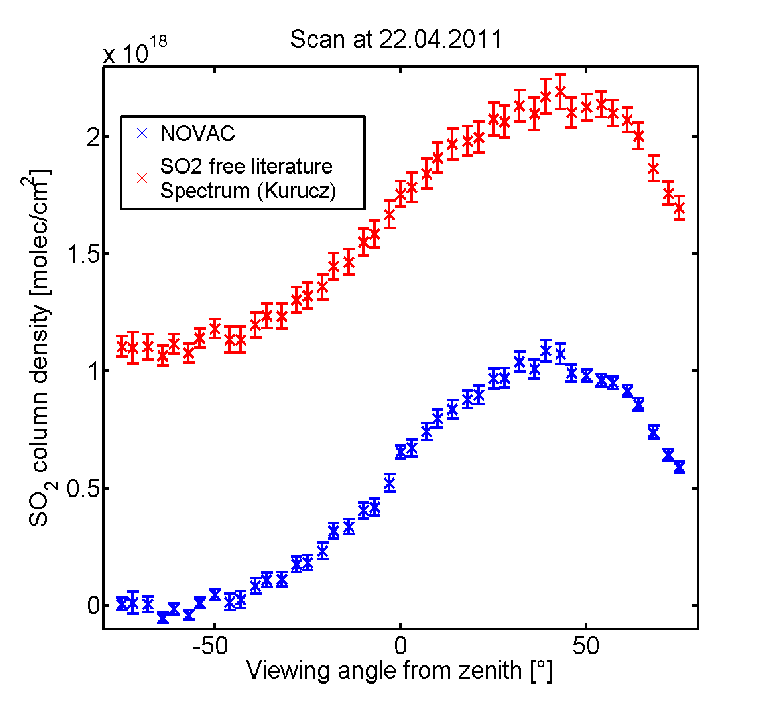
\includegraphics[width=0.7\linewidth]{Bilder/contaminated}
	\caption{Scan with a contaminated reference spectrum from April 2011. From \cite{WarnachSimon}}
	\label{fig:contaminated}
\end{figure}
If the reference region for any reason is
contaminated by volcanic trace gases, there are two possibilities: excluding the contaminated data from the evaluation or the reference spectrum has to be
replaced by a volcanic-gas-free reference. Alternative spectra are a
theoretical solar atlas spectrum or a volcanic-gas-free reference
spectrum recorded by the same instrument at another time.\\
A further possibility is to assume, that contamination only occurs for SO2, but not for BrO due to the smaller lifetimes of BrO, thus it is possible to use the Solar atlas spectrum for the \ce{SO2} evaluation, but the reference, recorded by the NOVAC-instrument at the same time for the BrO retrieval. Hereby the assumption, that BrO is not contaminated need to be proved. \\
%
\\
%
In the following we will discuss the two alternative reference spectra.
%
\subsection*{Evaluation using a Solar Atlas spectrum \label{kuruz}}
An alternative for choosing the region with the lowest column density as reference region is to use a theoretical high resolution solar atlas spectrum as reference \citep{chance2010improved}.
The use of a theoretical solar atlas spectrum as a reference which is completely volcanic-trace-gases-free was first proposed by \cite{salerno2009novel} and evolved by \citep{lubcke2014bro}.
The advantage of using a solar atlas spectrum as reference is, that we know that it is not affected by past or current volcanic gas emissions. Thus, it allows for a retrieval of the absolute trace gas SCDs in the volcanic gas plume. The disadvantage is, that using a solar atlas spectrum comes along with a drawback of precision: The spectral resolution of the theoretical solar atlas spectrum is much  higher than of the NOVAC instruments. Therefore the instrument functions would need to be perfectly modeled and added to the retrieval. This is not straight forward, because the instrumental line-shape varies over the wavelength region and is also mathmatically often not perfectly described by a simple approach like Gauss, lorents,..etc.\\ 
The reduction of precision is acceptable for the
\ce{SO2} retrieval but not suitable for a \ce{BrO} retrieval because then most data would be below the detection limit.\\
%
\\
%
Possible contaminations can be checked
by a theoretical solar atlas spectrum to evaluate the \ce{SO2} amount in the reference.\\

%
\subsection*{Evaluation using a spectrum of the same instrument}
An alternative reference spectrum could be a volcanic-gas-free reference
spectrum recorded by the same instrument at a different time. When using such a reference several problems occur:\\
As described in \Cref{NOVAC} the instruments used in NOVAC do not include features like temperature stabilization. Due to that the measurements are not independent of external parameters. 
So we need to choose a reference recorded at similar conditions with respect to meteorology and	radiation as well as in the temporal proximity due to instrumental changes with time and ambient conditions. Ideally the external conditions should be equal to the conditions at the time when the plume was recorded.\\
\\
%
When performing the evaluation with the Solar Atlas Spectrum as reference, finding the instrument function occur to be a central challenge. If the instrument function for the solar atlas spectrum is found the functions is typically used for a few years This could lead to higher errors due to an gradual worse matching instrument function.
Using the reference of the same instrument but recorded at another day, leads also to problems caused by different instrument functions, but compared to the calculated instrument function used for the evaluation with the solar atlas spectrum those differences in the instrument function could be smaller.
\\
In this work we combine both options in order to
achieve both, enhanced accuracy but still maximum possible precision of
the \ce{SO2} and \ce{BrO} retrievals. So we use the solar atlas spectrum to check for 
contamination and a reference spectrum recorded in temporal proximity by the same instrument as reference.\\
\\
If contamination occurs it is possible to choose a new reference from a list of gas free alternative references. In theory, for ideal instruments all references should lead to
	the same results for the gas retrievals. But instruments are imperfect (see Chapter
	4) thus the reference need to be chosen carefully in order to ensure reliable results.\\
%
\\
As discussed above it might occur, that the reference is contaminated for example by the plume of the day before.
%\textcolor{green}{das verstehe ich jetzt nicht - ich meine wenn wir jetzt das solar atlas spectrum nehmen ueberschaetzen wir ja , weil wir fahne von gestern und heute als eine einzige Fahne zusammen addieren...
%	unterschaetzung haben wir wenn der bei zum beispiel kleiner windgeschwindigkeit -> breite fahne das instrument in keiner richtung fahnen freien himmel sieht - oder bei hoher windgeschwindigkeit und instrument nah am berg die fahne so runtergedreuckt wird das das instrument in der fahne steht..: Florian : @ Nicole zur Überschätzung: wenn wir annehmen, dass die alte, bodennahe Fahne überall die gleiche Dicke hat und die neue Fahne eher im Zenit steht, dann ist der Anteil der alten Fahne zum neuen Gesamtsignal kleiner als der alten Fahne zum neuen Referenzsignal. D.h. Überschätzung ja, aber weniger als simple Addition.} 
If that happens, we underestimate the gas amount by using a contaminated reference. But another possibility is, that the plume itself is also contaminated. This might be the case if the volcanic gas of the volcano is not taken away by the wind, but accumulates at the instrument. If this is the case, using an other reference would lead to an overestimation of the column density of gases. With the data retrieved by the NOVAC instruments it is very difficult to discover whether the plume is contaminated or not. \\
\Cref{fig:contaminationdependencyso2} shows the strength of contamination as function of the mean \ce{SO2} amount of the day before. The strength of contamination is  measured as the difference between the evaluation for \ce{SO2} with a contaminated reference recorded at the same time as the plume spectrum was recorded and using a gas free reference. The data where fitted with a linear function. The left plot shows data from the Tungurahua volcano. In the right plot the data of Nevado Del Ruiz are visualized. Even though both plots show a slight increase of contamination strength with the mean amount of \ce{SO2} of the day before, the increase is not significant.\\
\textcolor{red}{hier waere es gut noch andere parameter zu testen - wie in Luebcke et al, zum beispile als funktion von Wind geschwindigkeit,..   Für NdR kann ich die Meteorologischen Daten ab 2014 beisteuern.}
\\
However this thesis is build on the assumption, that the plume is free of additional contamination \textcolor{yellow}{Nicole hat hier noch fragen, was ?}. In the following we discuss how to automatically determine an optimal reference from another scan.
\begin{figure}
	\subfigure{
	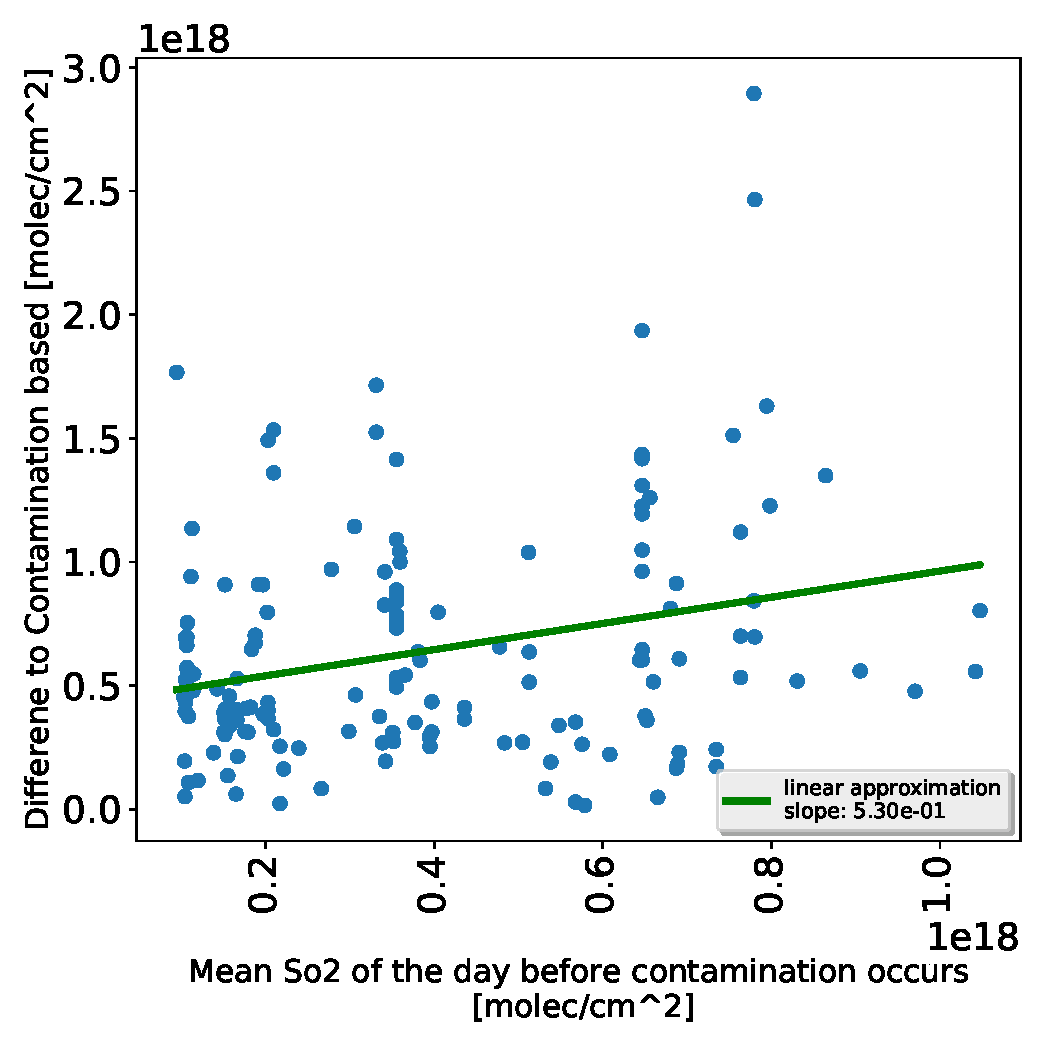
\includegraphics[width=0.5\linewidth]{Bilder/contaminationdependency_so2}}
\subfigure{
	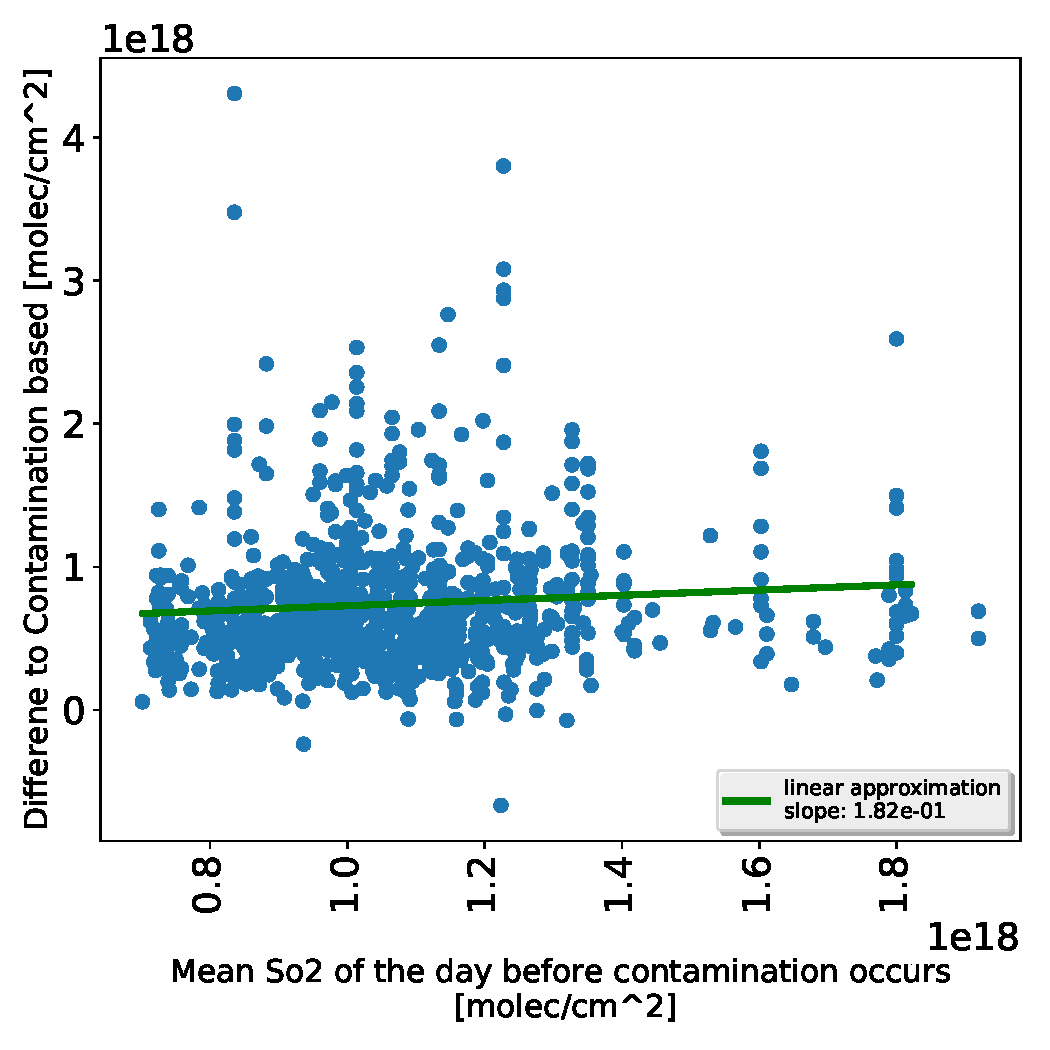
\includegraphics[width=0.5\linewidth]{Bilder/contaminationdependency_so2_Nevad}}
	\caption{The strength of contamination as function of the mean \ce{SO2} amount of the day before. The strength of contamination is defined as the difference in \ce{SO2} SCD  when evaluation with an alternative reference, or neglect the contamination. Left: data from Tungurahua. Right: data from Nevado Del Ruiz. \textcolor{red}{Wie wurde mean \ce{SO2} bestimmt? Wie sieht es bei max \ce{SO2} aus? (Und eigentlich müsse man ja eher die \ce{SO2} Emissionen anschauen. Die wir aber nicht (so einfach) kennen.)}}
	\label{fig:contaminationdependencyso2}
\end{figure}
		
	\part{Empirics}
	\chapter{\ce{BrO}  evaluation and its limitations}
	This chapter discusses the evaluation of the \ce{BrO} SCD , calculated from the spectra recorded by the spectroscopic instruments of NOVAC. The quality of the BrO retrieval hereby is defined by the BrO retrieval error.\\
\Cref{fig:allbroerrordistribution} shows the BrO "Multi Add"\footnote{More information about the multiadd-retrieval and the fit settings can be found in \Cref{Chap:evalroutine}} retrieval error distribution, which is centered around $1.1\cdot e^{+13}$ to $1.4\cdot e^{+13}$. \\
\\
The evaluation of the data from NOVAC are separated in the evaluation of \ce{SO2} and the evaluation of BrO. While the retrieval of \ce{SO2} is relatively easy due to the high amount of \ce{SO2} in the plume (magnitude of \ce{SO2} at Tungurahua $\approx 1e^{18}$), the \ce{BrO} evaluation is much more challenging due to not distinct BrO curves as a result of the lower BrO magnitudes (as can be seen in \Cref{fig:plumeref}). The magnitude of \ce{BrO} SCD is around $\approx 1e^{14}$. \\
%
\begin{figure}
	\subfigure{
		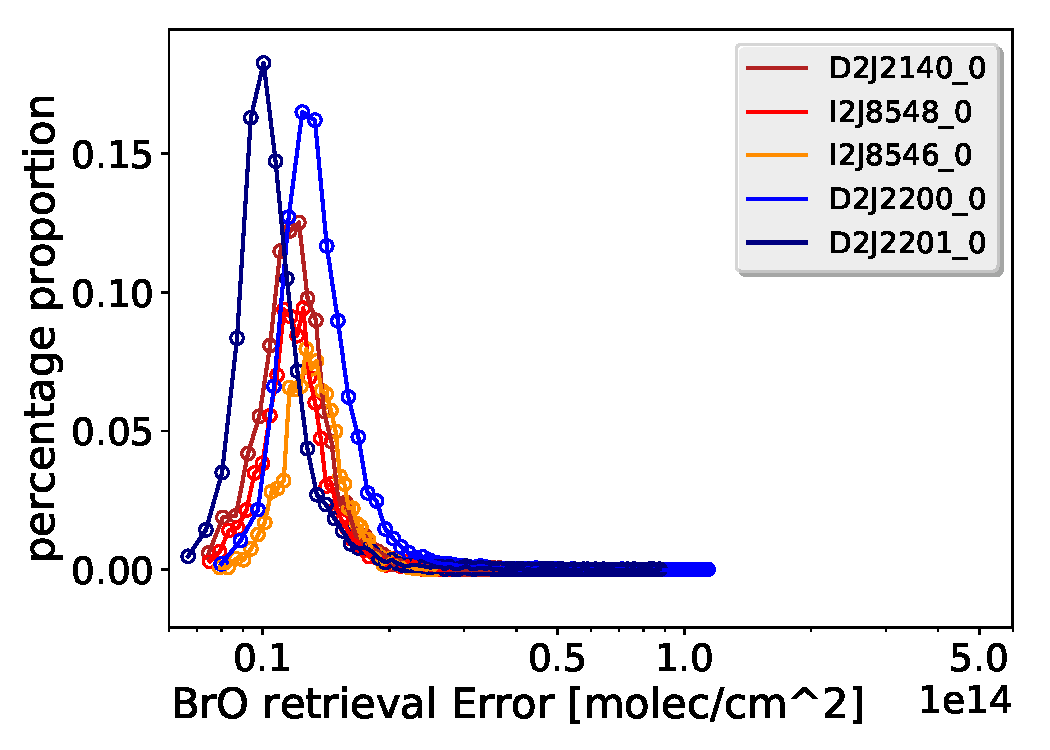
\includegraphics[width=0.49\linewidth]{Bilder/sametimeBrOErrorDistribution}}
	\subfigure{
		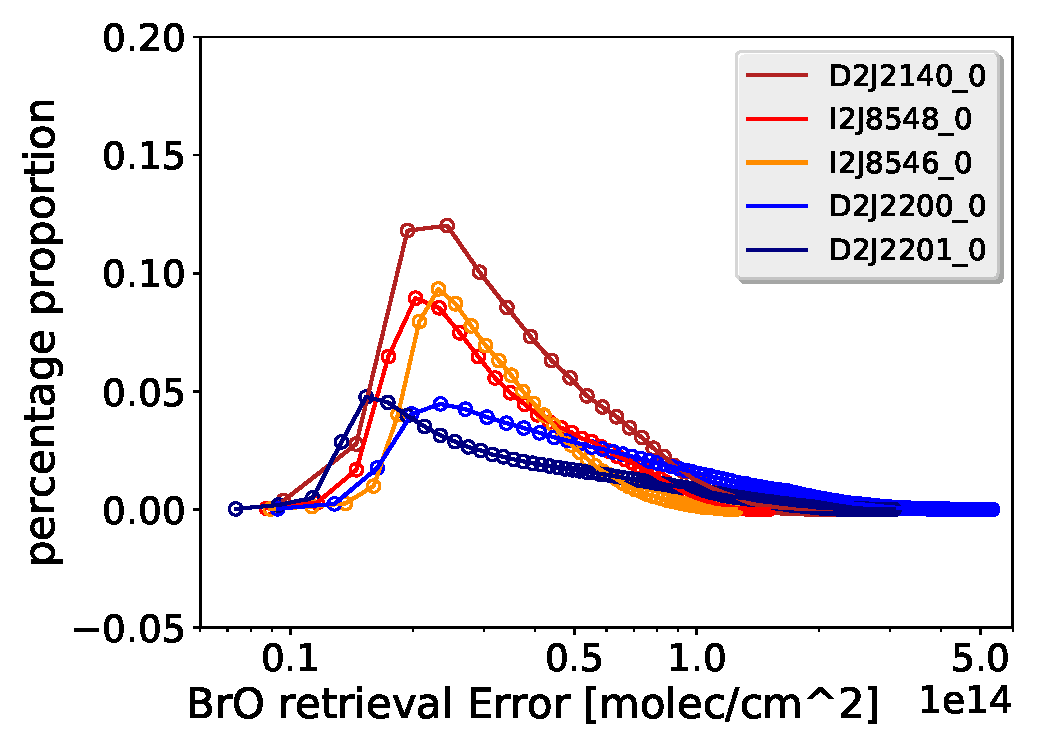
\includegraphics[width=0.49\linewidth]{E:/Masterarbeit/BrO_Error_Distribution/AllBrOErrorDistribution}}
	\caption{\ce{BrO} error distribution shown for all instruments considered in this thesis. The left plot shows the \ce{BrO} distribution for the "same time retrieval", the left plot shows the \ce{BrO} error distribution for the evaluation with a reference from another time, where the temporal difference between plume and reference is not longer that two weeks. The instruments of Nevado del Ruiz are coloured blue, while the the instruments of Tungurahua are coloured in yellow to red.
		The peaks for the single instrument are located at: D2J2140: 1.2$\cdot 10^{13}\frac{molec}{cm^2}$; I2J8548: 1.3$\cdot 10^{13}\frac{molec}{cm^2}$;
		I2J8546: 1.4$\cdot 10^{13}\frac{molec}{cm^2}$;
		D2J2200: 1.4$\cdot 10^{13}\frac{molec}{cm^2}$;
		D2J2201: 1.1$\cdot 10^{13}\frac{molec}{cm^2}$}
	\label{fig:allbroerrordistribution}
\end{figure}
%
This results in a larger uncertainty of the \ce{BrO}  SCD. Most of the \ce{BrO} data (98.3\% of the data) are below the detection limit of \ce{BrO}$_{err}$/\ce{BrO}$_{value}$<1/4. In comparison SCDs of \ce{SO2} in almost all cases (99.5\% of the data)  are above the detection limit. \\
%
Choosing a different reference spectrum than the reference measured at the same time as the plume in 99\% of all possible cases results in an increasing of the absolute error. 
Thus a \ce{BrO} error which is smaller than the "Same Time Error" is often not  possible to retrieve. 
However, for a contaminated same-time-reference the relative error might decrease due to the underestimation of the gas amount. \\
Due to the large uncertainty of \ce{BrO} relative to \ce{SO2} the optimization of the \ce{BrO} error is of particular importance. Therefore, the reference is chosen with respect to the \ce{BrO} error to maximize the quality of the \ce{BrO}/\ce{SO2} ratio. \\
\\
The amount of gas free alternative references is around 1500 per year. To make an optimal choice, it is necessary to examine the conditions which influence the \ce{BrO} retrieval.\\
Every spectrum is recorded under particular/unique ambient conditions. These measuring conditions generally are not equal for different scans. In our study, we show that references for which the surrounding conditions e.g temperature or cloudiness are equivalent with the surrounding conditions of the  plume measuring lead to a small error.\\
In the following, we take a closer look at the dependence of the \ce{BrO} error on external parameters. 
%
\subsubsection*{Data used for the analysis}
I evaluate a fixed plume spectrum using more than 1000 recorded multi add reference spectra in order to find the optimal reference spectrum. This evaluation is performed for more than 1000 multi add plume spectra in order to obtain a high statistical significance. Thus 1000 recorded "multi add" spectra result in $1000^2$ possible plume reference pairs and the coelrresponding differences in the external parameter and their associated \ce{BrO} error. 


\section{Influence of ambient conditions on the measurement \label{Chap:BROErr}}
The measurement and evaluation of the spectra monitored with NOVAC depends on the ambient conditions like temperature or cloudiness \citep{lubcke2014optical}.\\
Thus, the ambient conditions need to be taken into account for choosing a new reference.
\\
The ambient conditions that are considered in this thesis are written in \Cref{tab:externalparametters}
\begin{table}[h!]
	\centering
	\begin{tabular}{p{4cm}p{8.5cm}}
		%	\toprule
		Temporal difference &Temporal difference between measuring the plume and the reference.\\
		Daytime & Time of the day, and thus a measure of solar altitude.\\
		Temperature& The temperature of the instrument while recording the spectra.\\
		Colorindex&Ratio of two intensities at different wavelength as a measure for the cloudiness of the sky.\\
		Exposure time& Length of time the sensor of the NOVAC instrument is exposed to light.\\
		Elevation angle& Orientation of the instrument relative to the zenith, which corresponds to an elevation angle of zero degree.\\
		\label{tab:externalparametters}
	\end{tabular}
\end{table}	
%
The analysis of these external parameters are performed for spectra recorded at Tungurahua and Nevado del Ruiz. At Tungurahua three instruments with data recorded in the time span from July in 2008 to August in 2009 are used. Nevado del Ruiz contributes with two instruments in the time from the end of 2009 to the end of 2011.


\subsection{Strategy}

The external parameters described in \Cref{tab:externalparametters} are analyzed one by one in the following sections. Hereby I will proceed as follows:
A first step is to define a maximal temporal difference to prevent too large computational time.\\
The BrO measurement error as a function of the difference in the specific external parameter between the reference spectrum and the plume spectrum is shown for each of the individual instruments at Tungurahua and Nevado Del Ruiz. 
To quantify the dependency between the BrO retrieval error and the external parameter, the data are fitted with a first order polynomial for each of the individual instruments at Tungurahua and Nevado Del Ruiz. Hereby only the absolute differences were used. For every external parameter the fitting parameters slope and zero point are calculated.\\
Moreover, the correlation\footnote{See site \pageref{ff}}  between the BrO error and the absolute difference in the specific external parameter is calculated. If the BrO retrieval increases with increasing differences in surrounding condition between the plume spectra and the reference spectra, the difference, where the BrO retrieval error ($Mean(\Delta EP_{2})$)\footnote{EP: placeholder for any external parameter} is twice as high as for no difference is also calculated.\\  
Differences in external parameters can lead to large uncertainties in the retrieval, thus we analyze the amount of data possible references, if only data with differences smaller than ($Mean(\Delta EP_{2})$) in the specific external parameter are used. 
The advantage of restricting the accepted difference between the plume and the reference spectrum is a better control of the choice of the best reference. The disadvantage is that the amount of possible references decreases. Thus, it could occur that a reference is dismissed, which has a large difference in one parameter but is very similar in the remaining parameters.\\
The Mean, the corresponding standard deviation as well as the minimum and the maximum amount of references are calculated for each instrument.
\begin{center}
	\label{ff}
	\fbox{\parbox{13cm}{The Correlation coefficient $\rho_{X,Y}$ used in this thesis refer to the pearson product-moment correlation coefficients. It is a measure of linear correlation between two variables X and Y. The pearson correaltion coefficients range from -1 to +1.  Where +1 is total positive linear correlation,  -1 describes a total negative linear correlation, and a correlation of 0 refers to no linear correlation. The formula for the correlation coefficient is:
			\begin{equation*}
			\rho_{X,Y}=\frac{cov\left(X,Y\right))}{\sigma_X\sigma_Y}
			\end{equation*}
			were:
			$cov$  is the covariance\\
			$\sigma_X$ is the standard deviation of X\\
			$\sigma_{Y}$ is the standard deviation of Y\\
			Here the correlation is computed using the python\footnote{version 2.7.1} library Numpy (version 1.5.6)}}
	
\end{center}
%	
\subsection{Temporal difference}
%
\begin{figure}
	\centering
	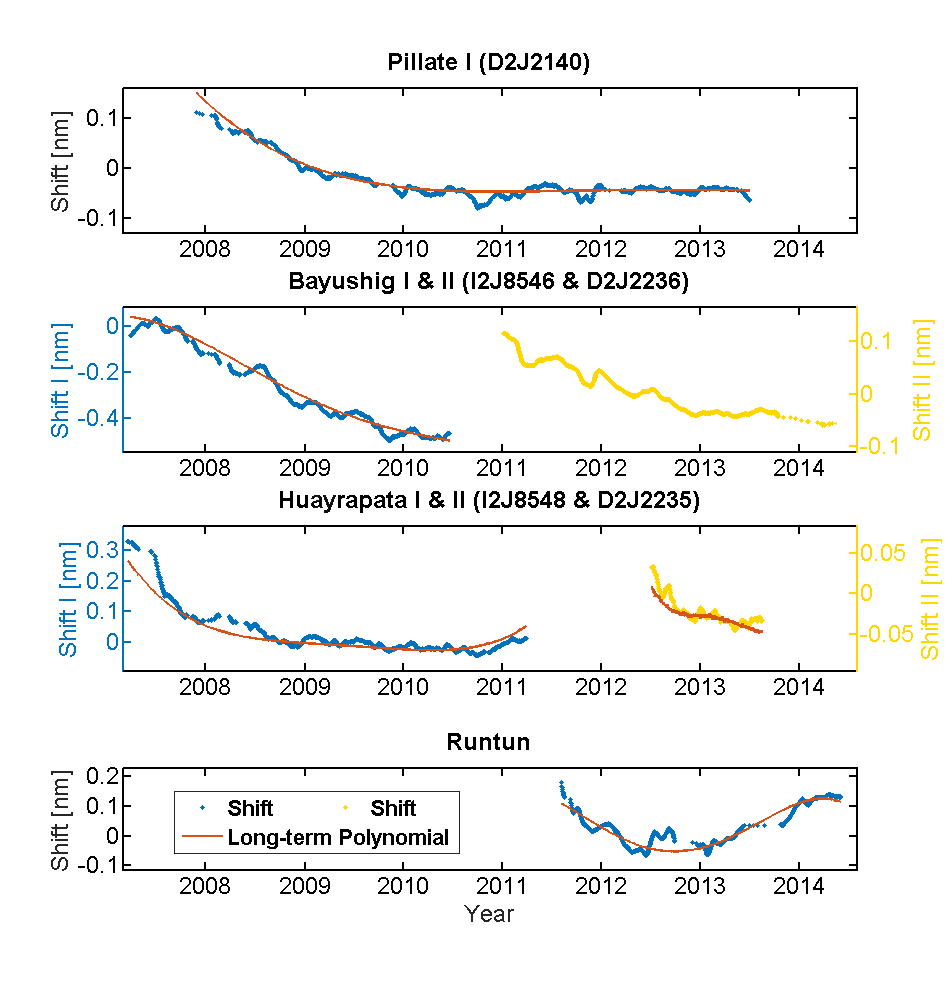
\includegraphics[width=1\linewidth]{Bilder/Simon/Bilder_Tung/Drift_Komplett_NEW}
	\caption{Wavelength shift over the time. The shift is shown for six NOVAC- instruments from Tungurahua. The red and yellow dots show the running mean over 20 days. Red line indicates a temperature independent long term polynomial. Source: \cite{WarnachSimon}}
	\label{fig:driftkomplettnew}
\end{figure}
%
\begin{figure}
	\subfigure[]{
		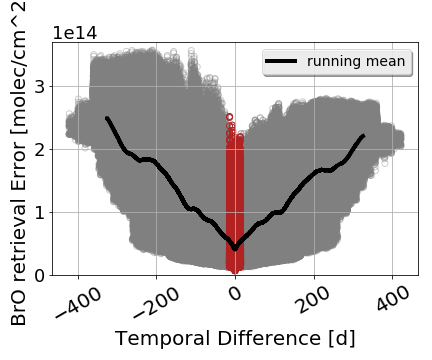
\includegraphics[width=0.5\linewidth]{Bilder/Datum}}
	\subfigure[]{
		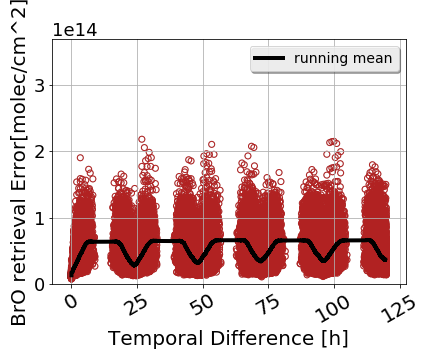
\includegraphics[width=0.5\linewidth]{Bilder/datumkurz}}	
	\caption{The \ce{BrO} error as a function of the temporal difference shown for the Pillate instrument from Tungurahua (2008-2009). The running mean is plotted with a black line. (a) Temporal differences up to 400 days. (b) Absolute temporal differences up to $\pm$ 120h. The periodical \ce{BrO}  error evolution indicates the impact of the daytime. }
	\label{fig:dat}
\end{figure}
%
\textcolor{red}{irgendwie stimmt hier was nicht noch mal SImons arbeit durchlesen oder sp}
Due to instrument drifts the fit quality decreases with the time difference between recording the plume and the reference. This could be a result of a wavelength shift over time observed by \citet{WarnachSimon}.  \citet{WarnachSimon} suggests that the drift is caused by a hysteresis effect. \Cref{fig:driftkomplettnew} shows the wavelength shift as a function of the time for six NOVAC instruments located at Tungurahua in the time between 2008 to 2014. In this thesis for the analysis data of Tungurahua between 2008 to the mid of 2009 are used. \Cref{fig:driftkomplettnew} shows a rather steep drift in this time interval.
\citet{WarnachSimon} observed a decrease of the shift after initial negative drift after the first two years at Pillate station. Thus we can observe an rather step drift at new installed instruments. Thus, it is observed that the temporal difference becomes less important after an initial adaptation on the surroundings after the installation of the instruments.\\
When using reference and plume spectra of the same time, these effects are cut out since the shift is equal for the plume and reference spectrum.\\
To examine the effect of the temporal difference on the retrieved \ce{BrO} error, for all reference-plume pairs the corresponding \ce{BrO} error is calculated. Due to the large amount of reference plume pairs within one year, it takes more than a month (Hardware details: Intel(R) Core(TM) i5-4570 CPU @ 3.20Ghz 64 Bit operating system, amount of 4 kernels) to evaluate the corresponding \ce{BrO} error for every possible reference-plume pair of one instrument. I did this for the  D2J2140 instrument installed at Tungurahua:\\
With the data from the D2J2140 instrument the dependency between the BrO retrieval error and the temporal difference between measuring the plume spectrum and the reference spectrum.\\
For an increasing temporal different between reference and plume measurement time the fit quality decreases on the average (On short timescales the influence of the temperature, daytime or other external parameter could be counteractive to the impact of the temporal distance). Thus a large temporal difference results in an increase of the \ce{BrO}  error of more than 600\% (see \Cref{fig:dat} (a)).
\ce{BrO} errors of such magnitudes are too large for our purposes. Therefore, it is useful to set a maximal temporal difference, to prevent too large \ce{BrO} error and to reduce the calculation time.
%
In \Cref{fig:dat} (a) it can be seen that the evolution of the \ce{BrO}  error with the temporal difference is symmetric around zero. Thus it is not necessary to distinguish between positive or negative temporal differences.
%The maximal temporal difference should be large enough to ensure a sufficient amount of references to be able to pick a reference with similar conditions. However, the maximal temporal difference should be small enough to prevent too large \ce{BrO} errors due to long term shifts.\\
\\
To evaluate the maximal time difference, for which we still get reliable results for every plume, where the "same time reference" is contaminated, the alternative reference is chosen, which leads to the minimal \ce{BrO} error.\\
% histogram
\begin{figure}
	\centering
	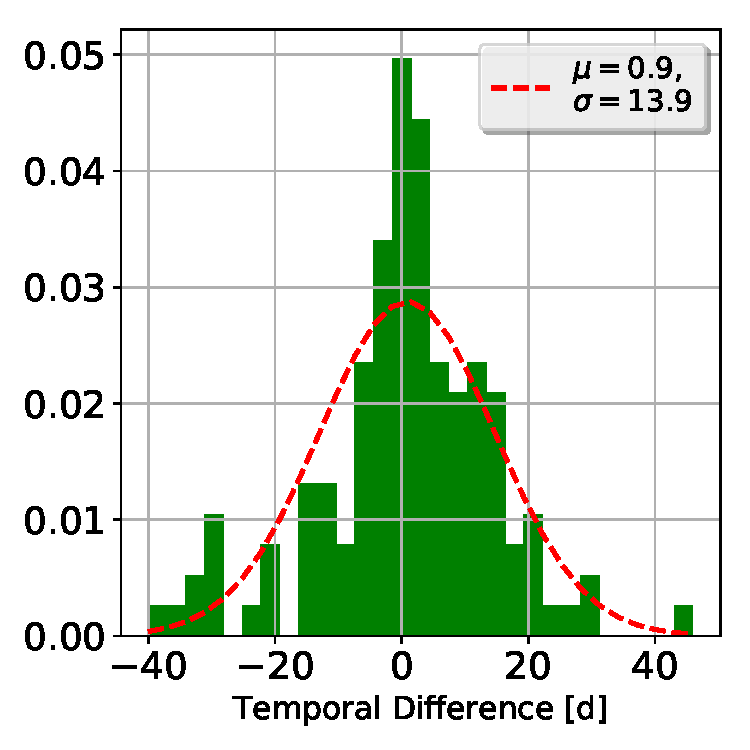
\includegraphics[width=0.6\linewidth]{Bilder/Hist}
	\caption{Histogram showing the frequency of getting the best reference as function of the temporal difference between plume and reference measuring. A Gaussian-like distribution is retrieved. The red dotted line visualizes a Gaussian fit for the shown histogram. The mean $\mu$ of the gaussian curve is: $\mu = 0.9$, the variance $\sigma$ is: $\sigma = 13.9$. The width of the green bars is three days.}
	\label{fig:Hist}
\end{figure}
%
In \Cref{fig:Hist} a histogram with the probability of picking the best reference as a function of the time difference is plotted. The mean of the Gaussian fitted on the data is slightly above zero. However the variance is calculated as approximately 14 days, thus a mean of 0.9 is statistical irrelevant. For the retrieval we allow all time differences within one sigma area. Thus, the maximal time difference is about two weeks.\\

% remaining possible reference spectra
\begin{table}[h]
	\centering
	\begin{tabular}{p{1.8cm}|p{2.15cm}p{2.15cm}p{2.15cm}p{2.15cm}p{2.15cm}|}
		%	\toprule
		Instrument	&D2J2140&I2J8546& I2J8548&D2J2200&D2J2201\\
		\toprule
		Mean&84.6 &163.7 &217.1&284.0 &225.6 \\
		\midrule
		Std&
		35.8&% $\equiv$ 100\%&
		29.9&% $\equiv$ 100\%&
		64.8&% $\equiv$ 100\%&
		69.5&% $\equiv$ 100\%&
		41.2\\% $\equiv$ 100\%\\
		\midrule
		Min&
		8 &%$\equiv$ 100\%&
		113&% $\equiv$ 100\%&
		97 &%$\equiv$ 100\%&
		64&% $\equiv$ 100\% &
		63\\% $\equiv$ 100\%\\
		\midrule
		Max&
		169&% $\equiv$ 100\%&
		214&% $\equiv$ 100\%
		399&% $\equiv$ 100\%
		433&%  $\equiv$ 100\%
		297\\% $\equiv$ 100\% \\
		\bottomrule
	\end{tabular}
	\caption{Amount of possible references when restricting the time span between plume and reference to two weeks. Here in the ”Mean” and “Std” row for each  instrument the average restriction is shown with the corresponding standard deviation. The “Min” and “Max” rows show the extend of restriction in the extreme cases (minimum and maximum amount of available references / restriction ratio).}
	\label{Tab:refstime}
\end{table}	
By restricting the temporal difference to 14 days, the amount of possible gas free references decreases to an average of 195 alternative references per contaminated plume (see \cref{Tab:refstime}). Hereby in the data considered in this thesis every plume has potential alternative reference spectra and the minimum amount of references is 8. However in general a plume without alternative references could occur.\\
If a continuous evaluation is required, this means the spectra are evaluated directly after the recording, the number of suitable gas free references halves since only references recorded before the plume are available.\\
For the following analysis of the remaining external parameters all temporal differences are below 14 days.\\
\\
\begin{figure}
	\centering
	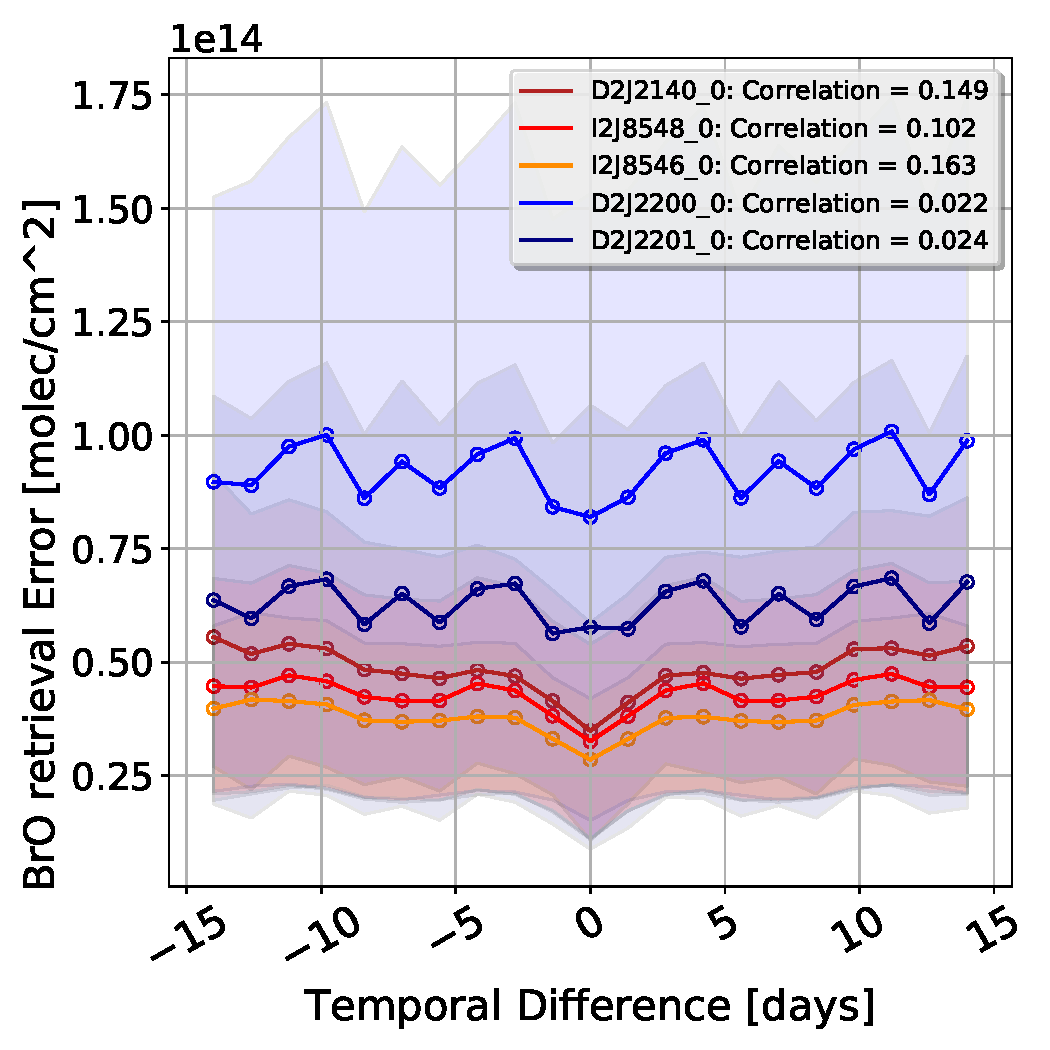
\includegraphics[width=0.7\linewidth]{Bilder/DatallInstruments}
	\caption{The \ce{BrO} measurement error as a function of the temporal difference in days between the reference and the plume is shown for each of the individual instruments at Tungurahua and Nevado del Ruiz. The instruments at Nevado del Ruiz are coloured in blue, while the instruments at Tungurahua are coloured in red colour tones.  To evaluate the plume spectra all reference spectra with a temporal distance of no longer than two weeks are used. An increase of the \ce{BrO} error with the absolute difference in temperature is observable. This is quantified by a correlation between the \ce{BrO} retrieval error and the absolute temporal difference. The plots reveal a symmetry around the axis with zero temperature difference.}
	\label{fig:datallinstruments}
\end{figure}
%
\Cref{fig:dat} (b) shows the evolution of the \ce{BrO} error for a maximal absolute temporal difference of 120 hours. It is only possible to record data during daytime. This causes the lack of data in the night time. A periodic decrease of the \ce{BrO} error can be seen. This is a result of a decrease of the \ce{BrO} error when the ambient conditions coincidence. In this case the daytime coincidence causes the \ce{BrO}  error decrease. This effect is analysed in detail in the following.


\subsection{ Daytime \label{chap:daytime}}
\begin{figure}
	\centering
	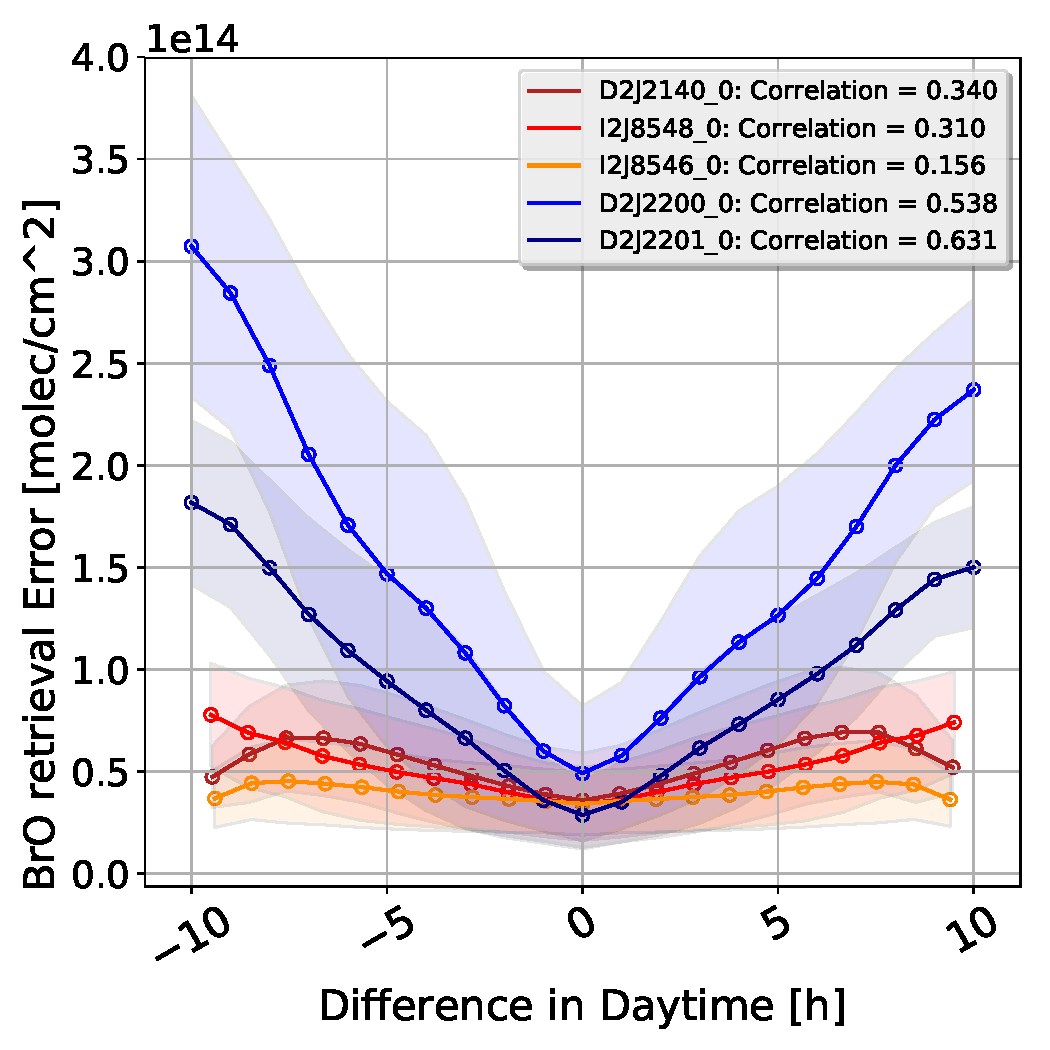
\includegraphics[width=0.7\linewidth]{Bilder/DiffDaytimeallInstruments}
	\caption{The \ce{BrO} measurement error as a function of the difference of daytime between the reference and the plume is shown for each of the individual instruments at Tungurahua and Nevado del Ruiz. To evaluate the plume spectra all reference spectra with a temporal distance of no longer than two weeks are used. An increase of the \ce{BrO} error with the absolute difference in daytime is observable. This is quantified by a correlation between the \ce{BrO} retrieval error and the absolute difference in daytime. The plots reveal a symmetry around axis with zero daytime difference. }
	\label{fig:diffdaytime}
\end{figure}
% individual text
Here I discuss the dependency of the BrO retrieval error based on the bulk effect of a difference in daytime. During the day a lot of external parameters like temperature, solar zenith angle etc. change. In particular, the solar zenith angle could have an impact on the fit quality since the light path of the sun is much longer in the morning or evening compared to the noon. Therefore, the scattering effects and the light intensity are different for both spectra.\\

% fig_curves
In \Cref{fig:diffdaytime} the \ce{BrO} error is plotted against the daytime difference between the plume spectrum and the reference spectrum.  \\
Because of the observed symmetry around zero the absolute daytime difference is used for the fit. The computed fitting parameters slope and intercept for each instrument are shown in \Cref{tab:dtcalc}. \\
%
As it can be seen in \Cref{tab:dtcalc}, the intercepts, which defines the main BrO retrieval error for a daytime difference of zero, vary at Tungurahua between 3.28$\cdot10^{13}\frac{molec}{cm^2}$ and 3.43$\cdot10^{13}\frac{molec}{cm^2}$. The variation at Nevado del Ruiz ranges from  2.24$\cdot10^{13}\frac{molec}{cm^2}$ to 4.01$\cdot10^{13}\frac{molec}{cm^2}$. \\
The correlation coefficient between daytime und BrO error 
ranges from 0.156 for the instrument I2J8546 to  0.631 for D2J2201 and exhibits a large variation between the instruments. This lead to the conclusion, that the dependence of the fit quality on the daytime depends largely on the location of the instrument.\\
The $\Delta DT_{2}$, the daytime difference for which the BrO retrieval error doubles compared to a daytime difference of zero is rather high for the instruments installed at Tungurahua (6.8h to 24.2h) and rather low for the instruments installed at Nevado del Ruiz (11.62h to 1.9h).

% tab_fit CAPTION
\begin{table}[h]
	\centering
	\begin{tabular}{|p{2cm}|p{2.15cm}|p{2.15cm}|p{2.15cm}|p{2.15cm}|p{2.15cm}|}
		%	\toprule
		Instrument	&D2J2140&I2J8546& I2J8548&D2J2200&D2J2201\\
		\toprule
		Slope&5.07$\cdot$ e+12&1.40$\cdot$ e+12 &3.77$\cdot$ e+12 &2.04$\cdot$ e+13& 1.38$\cdot$ e+13\\
		\midrule
		Correlation&
		0.340&
		0.156&
		0.310&
		0.538&
		0.631\\
		\midrule
		Intercept& 3.43$\cdot$ e+13&3.39$\cdot$ e+13&3.28$\cdot$ e+13&  4.01$\cdot$ e+13&  2.24$\cdot$ e+13\\
		\midrule
		$\Delta DT_{2}$&6.8&24.2&8.7&1.9&1.62\\
		\bottomrule
	\end{tabular}
	\label{tab:dtcalc}
	\caption{The \ce{BrO} measurement error as a function of the difference of daytime in hours between the reference and the plume is fitted with a first order polynomial for each of the individual instruments at Tungurahua and Nevado del Ruiz. This table shows the fitting parameters slope and intercept. Moreover, the correlation between the \ce{BrO} error and the absolute daytime difference is shown. In the $\Delta DT_{2}$ row the daytime difference for which the error doubles compared to a daytime difference of zero is shown.}
\end{table}

% tab_ratio CAPTION
\begin{table}
	\centering
	\begin{tabular}{p{1.8cm}|p{2.15cm}|p{2.15cm}|p{2.15cm}|p{2.15cm}|p{2.15cm}}
		%	\toprule
		Instrument	&D2J2140&I2J8546& I2J8548&D2J2200&D2J2201\\
		\toprule
		Mean&
		72.0 ($\entspricht\,$85.1\%) &		147.4 ($\entspricht\,$90.0\%)&
		198.4 ($\entspricht\,$91.4\%)&		275.0 ($\entspricht\,$96.8\%)&
		205.8 ($\entspricht\,$91.2\%)\\
		\midrule
		Std&		31.87 ($\entspricht\,$89.0\%)&32.0 ($\entspricht\,$107.0\%)&
		71.0 ($\entspricht\,$109.5\%)&		70.8 ($\entspricht\,$101.8\%)&
		50.1 ($\entspricht\,$121.6\%) \\
		\midrule
		Min&
		6 $\qquad$($\entspricht\,$75.0\%)&		58 ($\entspricht\,$51.3\%)
		&91 ($\entspricht\,$93.8\%)		&54 ($\entspricht\,$84.4\%)
		&45 ($\entspricht\,$71.4\%)\\
		\midrule
		Max&
		160 ($\entspricht\,$94.7\%) &
		214 ($\entspricht\,$100\%) &
		399 ($\entspricht\,$100\%) &
		433 ($\entspricht\,$100\%) &
		297 ($\entspricht\,$100\%) \\
		\bottomrule
	\end{tabular}
	\caption{This table shows the absolute amount and the percentage corresponding to initial number of references without any restrictions of ambient conditions (table 6.1) of remaining references if restricting the daytime difference to the mean $\Delta DT_{2}$ over all instruments except I2J8546 due to the large uncertainty ($Mean(\Delta DT_{2}) = 4.75h$). Here in the ”Mean” and “Std” row for each  instrument the average restriction is shown with the corresponding standard deviation. The “Min” and “Max” rows show the extend of restriction in the extreme cases (minimum and maximum amount of available references / restriction ratio).}
	\label{tab:daytimerest}
\end{table}	
% tab_ratio
The mean ($Mean(\Delta DT_{2})$) is calculated without taking the instrument I2J8546 into account due to the low correlation of 0.156. Using the I2J8546 instrument as well would lead to an  $Mean(\Delta DT_{2})$ of $8.6h$, thus, the restriction would not have any influence, since the maximal time difference is limited to the time where the sun is shining.\\ 
Excluding references with daytime differences above $4.75$h restricts the amount of potential references to $85.1\%$ for D2J2140 to $96.8\%$ for D2J2200. In extreme cases a restriction down to $51.3\%$ of the entire set of references can occur (see \Cref{tab:daytimerest}).



\subsection{Temperature}
% fig_curves CAPTION
\begin{figure}
	\centering
	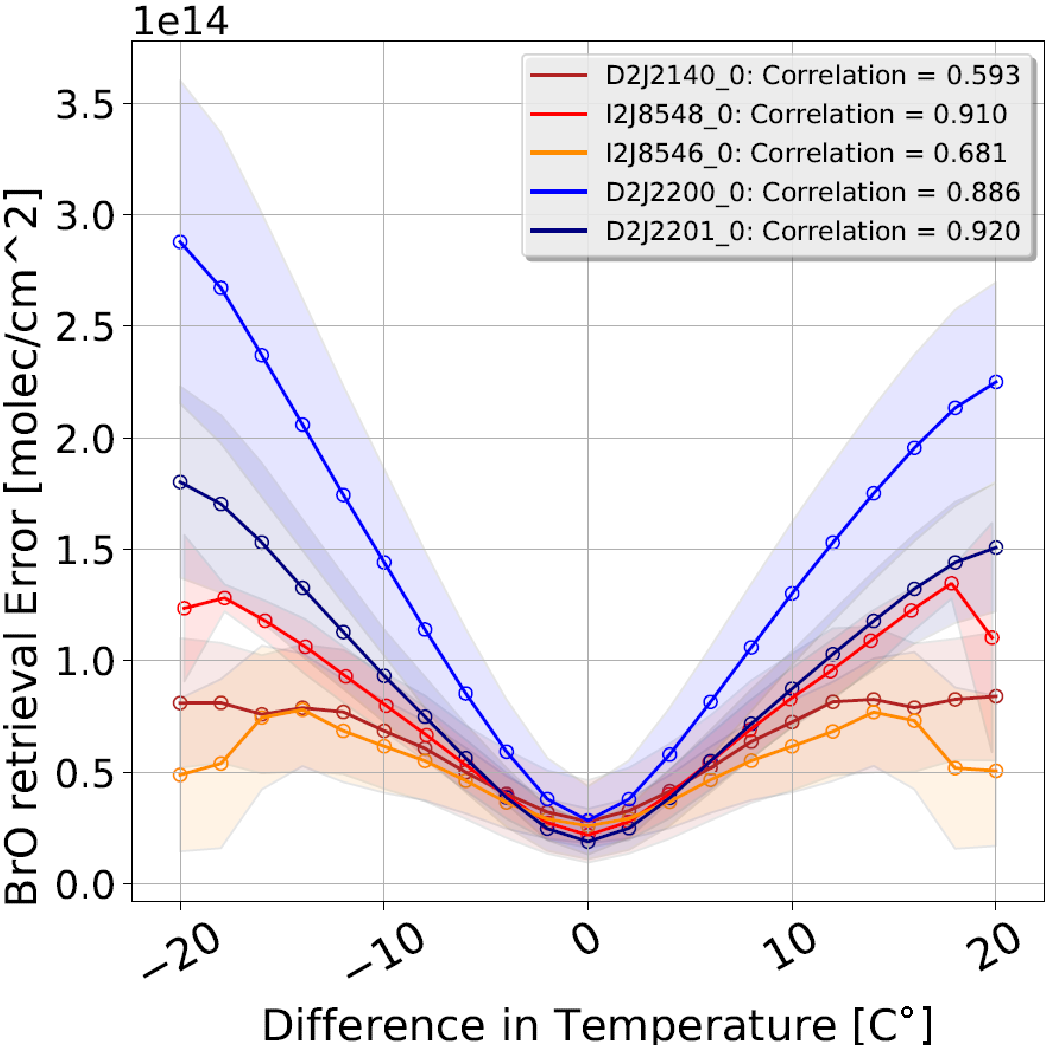
\includegraphics[width=0.7\linewidth]{Bilder/DiffTempallInstruments1}
	\caption{The \ce{BrO} measurement error as a function of the difference of temperature between the reference and the plume is shown for each of the individual instruments at Tungurahua and Nevado del Ruiz. To evaluate the plume spectra all reference spectra with a temporal distance of no longer than two weeks are used. An increase of the \ce{BrO} error with the absolute difference in temperature is observable. This is quantified by a correlation between the \ce{BrO} retrieval error and the absolute difference in temperature. The plots reveal a symmetry around the axis with zero temperature difference.}
	\label{fig:difftemp}
\end{figure}
% individual text
In this section I discuss the particular effect of a difference in temperature, which has been shown to be the most important influence.
The instrument design of the NOVAC instruments compromises between accuracy and robustness as explained in \Cref{NOVAC}. In particular, there are no internal thermal stabilizations installed as an attempt to reduce the instruments power consumption and increase the robustness. This can influence the recorded spectra.\\
The ambient temperature however has an influence on the optical adjustment of the NOVAC instrument and thus on the instrument line function and calibration of the spectrometer.
The calibration for the wavelength to pixel mapping (WPM) is commonly determined by a mercury lamp or by the comparison with the high defined Kuruz spectrum.
As the WPM depends on the optical alignment of the spectrometer, which itself depends on the temperature, it is not constant.
Changes in the spectrometers temperature can cause changes in the instrument line function and shifts in the WPM (\citep{pinardi2007influence}). 
% short term wavelength
\begin{figure}		
	\subfigure[]{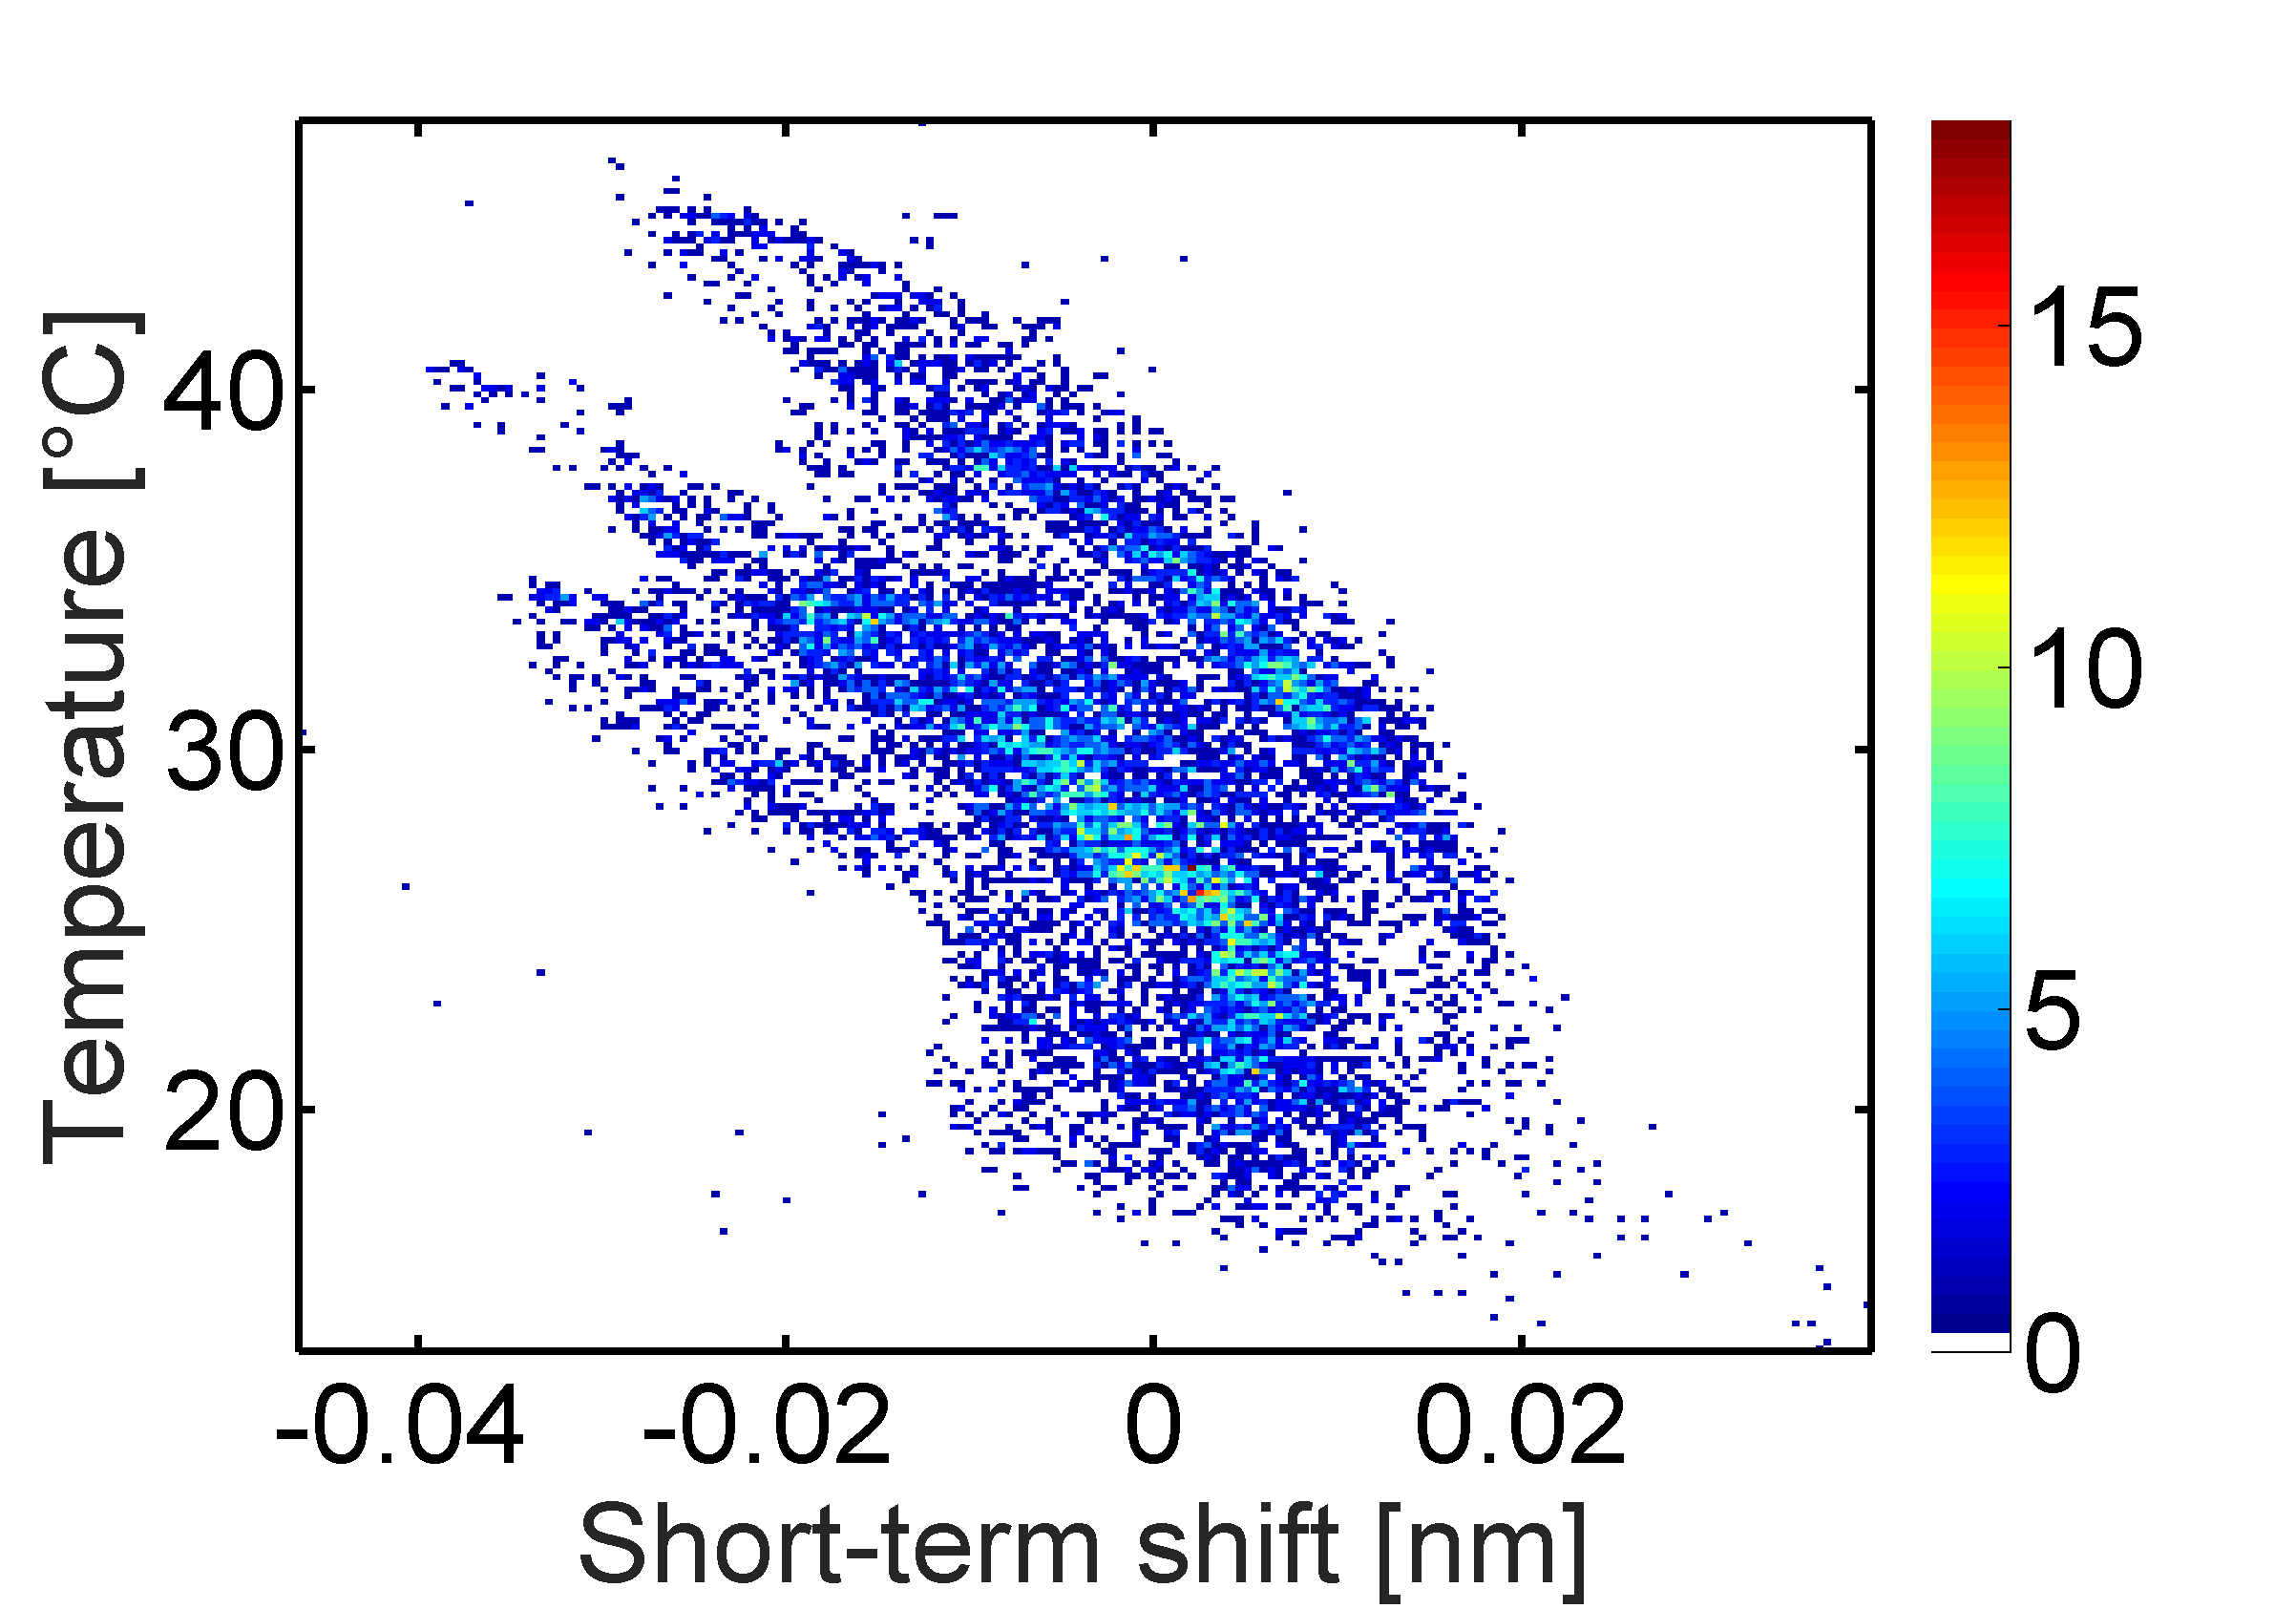
\includegraphics[width=0.49\textwidth]{Bilder/Simon/Bilder_Tung/D2J2140_Before}}
	\subfigure[]{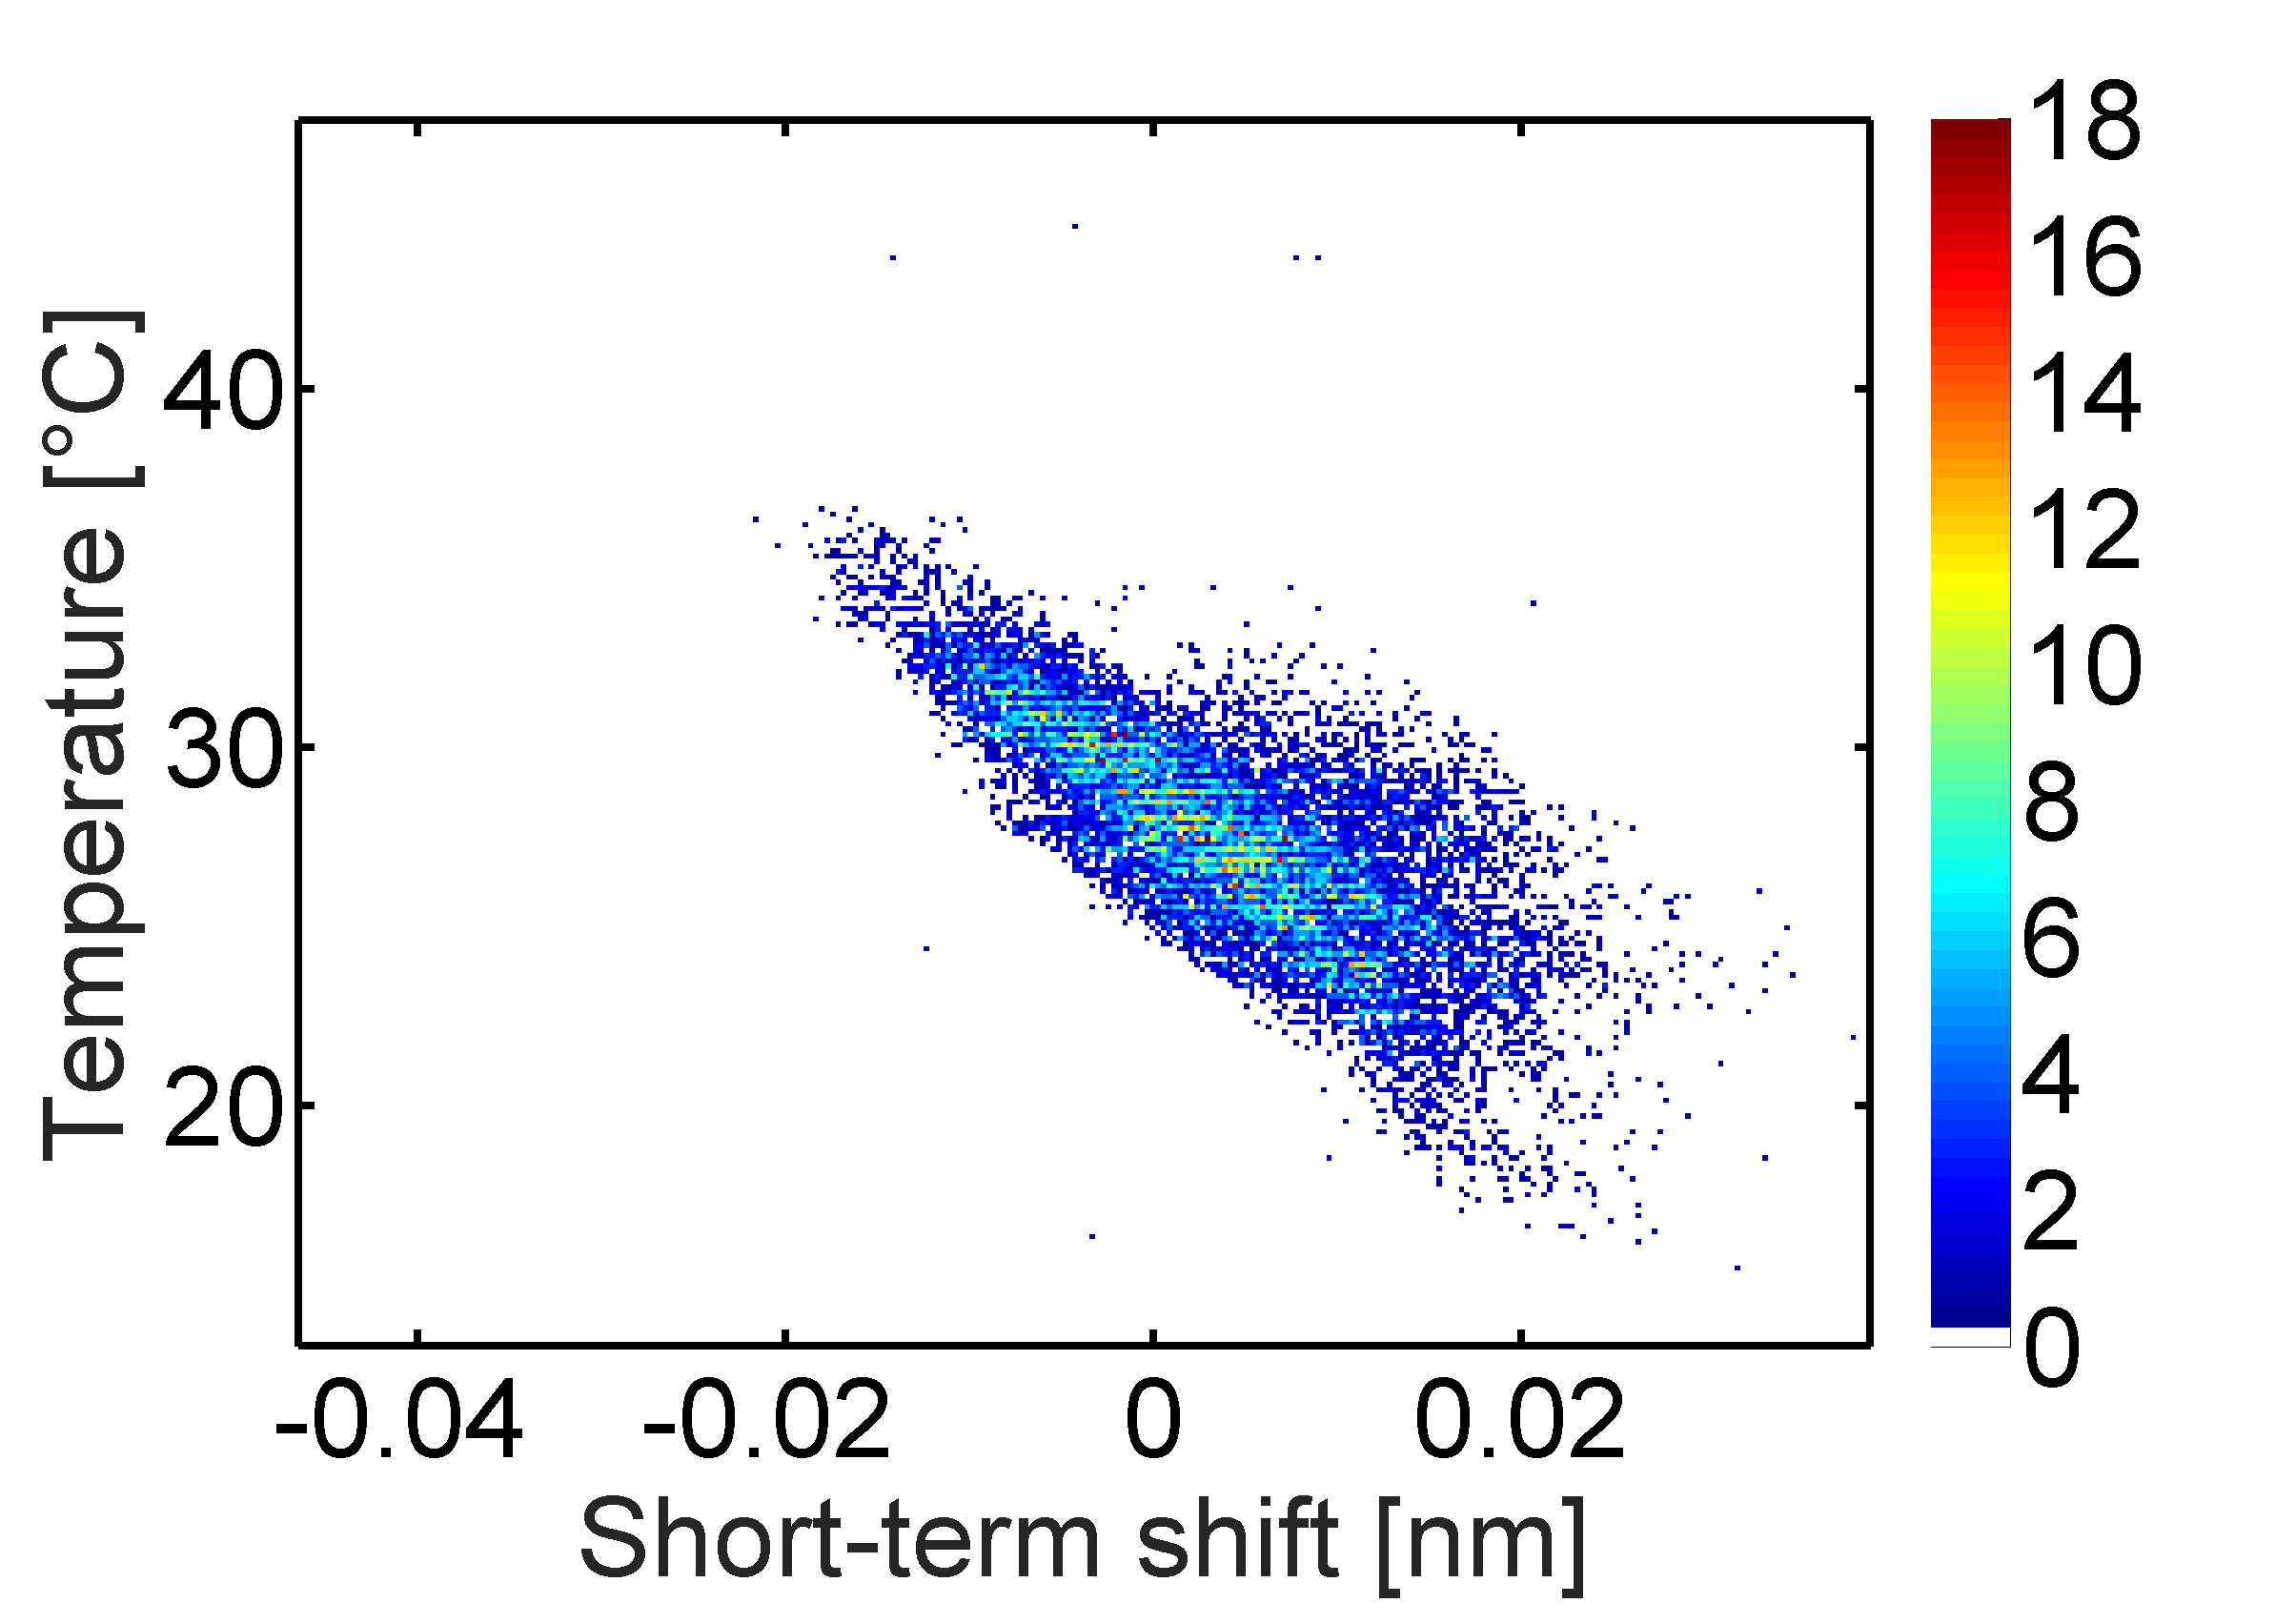
\includegraphics[width=0.49\textwidth]{Bilder/Simon/Bilder_Tung/D2J2140_After}}
	\caption{Short term wavelength as a function of the instrument temperature for Pillate 1. The coloring of the scatter points indicate the temporal evolvement. (a) initial period prior to January 2010 (b) after 2010. Source: \cite{WarnachSimon}.}
	\label{fig:shorttermshift}
\end{figure}
Moreover, \cite{WarnachSimon} show that, short term shifts are related to the instrument temperature (see \Cref{fig:shorttermshift}).\\
The above discussed temperature dependence of the WPM causes a reduction of the fit quality with increasing instrument temperature difference between plume and reference (see \Cref{fig:difftemp}). Thus, the \ce{BrO} error also increases with the temperature difference.
Compared to the other external parameters the temperature difference has the largest impact on the \ce{BrO} error.\\
\\
% tab_fit CAPTION
\begin{table}[h]
	\centering
	\begin{tabular}{|p{2cm}|p{2cm}|p{2cm}|p{2cm}|p{2cm}|p{2cm}|}
		%	\toprule
		Instrument	&D2J2140&I2J8546& I2J8548&D2J2200&D2J2201\\
		\toprule
		Slope&4.10$\cdot$ e+12 &3.93$\cdot$ e+12 &6.50$\cdot$ e+12 &1.24$\cdot$ e+13&8.17$\cdot$ e+12 \\
		\midrule
		Correlation
		& 
		0.593& 
		0.681& 
		0.910& 
		0.886& 
		0.920\\
		\midrule
		Intercept&2.58$\cdot$ e+13&2.23$\cdot$ e+13&1.60$\cdot$ e+13& 1.38$\cdot$ e+13& 9.07$\cdot$ e+12\\
		\midrule
		$\Delta T_{2}$&6.3&5.7&2.5&1.1&1.1\\
		\bottomrule
	\end{tabular}
	\label{tab:tempe}
	\caption{The \ce{BrO} measurement error as a function of the difference of temperature between the reference and the plume is fitted with a first order polynomial for each of the individual instruments at Tungurahua and Nevado del Ruiz. This table shows the fitting parameters slope and intercept. Moreover, the correlation between the \ce{BrO} error and the absolute temperature difference is shown. For the temperature difference this correlation with an average of $0.797$ is the highest compared to the other external parameters. In the $\Delta T_{2}$ row the temperature difference for which the error doubles compared to a temperature difference of zero is shown. This is already the case for a difference of $3.3^\circ C$}
\end{table}
% tab_fit
% fig_curves
The plots reveal a symmetry around axis with zero temperature difference (see \Cref{fig:difftemp}), thus using only the absolute temperature difference for the fit is reasonable.\\
The intercepts for the BrO error at Tungurahua vary from 1.6$\cdot10^{13}\frac{molec}{cm^2}$ to 2.58$\cdot10^{13}\frac{molec}{cm^2}$ (see \Cref{tab:tempe}). The intercepts at Nevado del Ruiz are lower and ranges from  9.07$\cdot10^{12}\frac{molec}{cm^2}$ to 1.38$\cdot10^{13}\frac{molec}{cm^2}$. The $\Delta T_{2}$ from the data of Tungurahua (2.5 K to 6.3K) are significantly higher as at Nevado del Ruiz (1.1 K). The mean $\Delta T_{2}$ is $ 3.3$K. The conclusion is, that the Temperature has a stronger influence at the Nevado del Ruiz volcano.\\
The correlation between the \ce{BrO} error and the absolute temperature difference has a high significants. 
The correlation coefficients ranges from 0.593 for the instrument D2J2140 to  0.92 for D2J2201 and exhibits a large variation between the instruments. \\
The computed fitting parameters slope and intercept for each instrument are shown in \Cref{tab:tempe}.\\
% tab_ratio CAPTION
\begin{table}
	\centering
	\begin{tabular}{|p{1.8cm}|p{2.15cm}|p{2.15cm}|p{2.15cm}|p{2.15cm}|p{2.15cm}|}
		%	\toprule
		Instrument	&D2J2140&I2J8546& I2J8548&D2J2200&D2J2201\\
		\toprule
		Mean&
		39.6 ($\entspricht\,$46.8\%)&
		119.3 ($\entspricht\,$72.9\%)
		&158.2 ($\entspricht\,$72.9\%)
		&233.6 ($\entspricht\,$82.3\%)
		&151.6 ($\entspricht\,$67.2\%)\\
		\midrule
		Std&
		24.7 ($\entspricht\,$68.9\%)&
		50.4 ($\entspricht\,$168.6\%)&
		76.0 ($\entspricht\,$117.2\%)&
		84.5 ($\entspricht\,$121.6\%)&
		72.6 ($\entspricht\,$176.2\%)\\
		\midrule
		Min&
		1 ($\entspricht\,$12.5\%)
		&8 ($\entspricht\,$7.1\%)&
		12 ($\entspricht\,$12.4\%)&
		3 ($\entspricht\,$4.7\%) &
		6 ($\entspricht\,$9.5\%)\\
		\midrule
		Max
		&
		130	 ($\entspricht\,$76.9\%)&
		213	 ($\entspricht\,$99.5\%)&
		386 ($\entspricht\,$96.7\%)&
		414	 ($\entspricht\,$95.6\%) &
		296	 ($\entspricht\,$99.7\%)\\
		\bottomrule
	\end{tabular}
	\caption{This table shows the absolute amount and the ratio (to \Cref{Tab:refstime}) of remaining references if restricting the temperature difference to the mean $\Delta T_{2}$ over all instruments ($Mean(\Delta T_{2}) = 3.3^{\circ}C$). Here in the ”Mean” and “Std” row for each  instrument the average restriction is shown with the corresponding standard deviation. The “Min” and “Max” rows show the extend of restriction in the extreme cases (minimum and maximum amount of available references / restriction ratio).}
	\label{tab:decTemp}
\end{table}	
% tab_ratio
If restricting the temperature difference to the mean $\Delta T_{2}$ over all instruments ($Mean(\Delta T_{2}) = 3.3$) the amount of possible references decrease as shown in \Cref{tab:decTemp}. Excluding references with temperature differences above $Mean(\Delta T_{2}) = 3.3$ restricts the amount of potential references to $46.8\%$ for the $D2J2140$ instrument to $82.3\%$ for the $D2J2200$ instrument.

\subsection{ Colorindex}
\begin{figure}
	\centering
	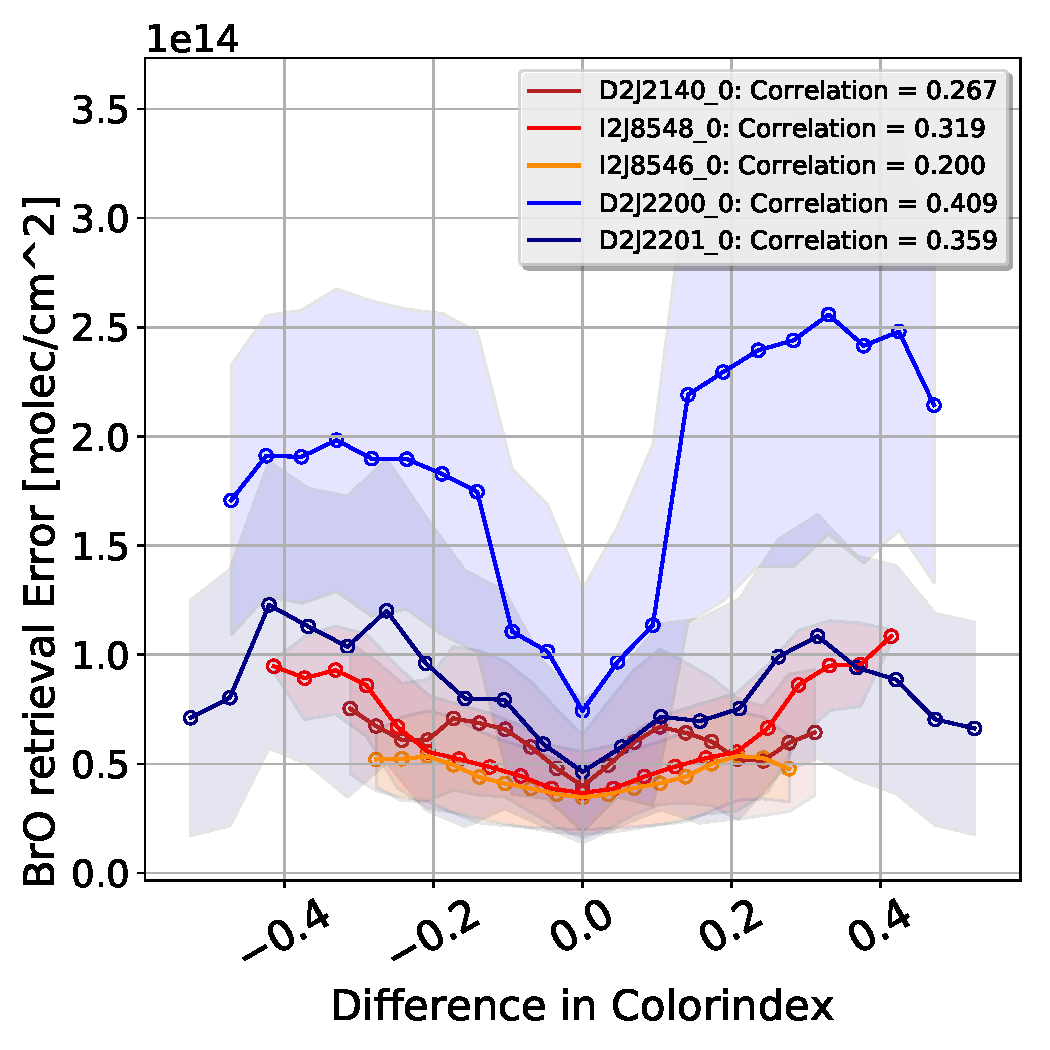
\includegraphics[width=0.7\linewidth]{Bilder/DiffColidxallInstruments}
	\caption{The \ce{BrO} measurement error as a function of the difference of colorindex between the reference and the plume is shown for each of the individual instruments at Tungurahua and Nevado del Ruiz. To evaluate the plume spectra all reference spectra with a temporal distance of no longer than two weeks are used. An increase of the \ce{BrO} error with the absolute difference in colorindex is observable. This is quantified by a correlation between the \ce{BrO} retrieval error and the absolute difference in colorindex. The plots reveal a symmetry around axis with zero colorindex difference. }
	\label{fig:diffcolidx}
\end{figure}
% individual text
Clouds  have  a  strong  influence  on  the  atmospheric  radiative  transfer  and  thus  affect  the  interpretation  and  analysis of DOAS \citep{wagner2014cloud}.
Clouds can be identified by several measurement quantities which they influence.
As Mie scattering is dominant in clouds the wavelength dependency of the light that is scattered is different than the Rayleigh sky. Thus, clouds can be easily identified by their white color.
Therefore, the cloudiness of the sky can be quantified in a scalar measure defined by the ratio of the measured intensity at two wavelengths, the so-called colour index.
\cite{wagner2014cloud} showed that for a zenith-looking instrument the measured radiation intensity is enhanced by clouds. Thus, clouds can cause large errors for the retrieved gas column density and the corresponding uncertainties. 
Cloud effects are especially severe if the cloudiness for the recorded plume and reference spectra strongly defer. Also for broken clouds the described effect can be observed as measurements at some elevation angles might be influenced by clouds while others are not.
In this work we use the Colour Index (CI) between the intensities at 320nm and 360 nm.
These two wavelengths are as far apart as the filter used for stray-light prevention in the spectrometers allows.
%% I don’t understand 	
On the other hand, the lower wavelength avoids the deep UV range where \ce{SO2} and  \ce{O3} absorption plays a dominant role.
%% I don’t understand 	
The Mie scattering in the clouds is responsible for the higher amount of radiation from larger wavelengths. This results in a decrease of the CI which was observed for NOVAC instruments by \citet{lubcke2014optical}.\\
We evaluated the CI at the zenith. To increase the stability of the fit we add 10 the intensities from 10 consecutive spectra. Using always the zenith to evaluate the colour index makes the colour index more comparable, but if broken clouds occur, the CI of the reference and the plume could differ from the calculated CI of the zenith. This could be a reason for the large deviations of the mean \ce{BrO} error as function of the colour index (see \Cref{fig:diffcolidx})\\
% fig_curves
In \Cref{fig:diffcolidx} the \ce{BrO} error is plotted against the colorindex difference between the plume and the reference spectrum. The plot is done similar as the plots for the temperature.
The plots mostly reveal a symmetry around the zero colorindex difference-axis. Thus, the absolute colorindex can be used for the fitting which is done equivalently to the analysis of the temperature and the daytime. The computed fitting parameters slope and intercept for each instrument are shown in \cref{tab:colidxcalc}. \\
The intercepts at Tungurahua vary from 3.36$\cdot10^{13}\frac{molec}{cm^2}$ to 4.01$\cdot10^{13}\frac{molec}{cm^2}$. The variation at Nevado del Ruiz ranges from  4.74$\cdot10^{13}\frac{molec}{cm^2}$ to 7.21$\cdot10^{13}\frac{molec}{cm^2}$.\\
The correlation is as well calculated and ranges from 0.2 for the instrument I2J8546 to  0.409 for D2J2200.\\
\begin{table}[h]
	\centering
	\begin{tabular}{|p{2cm}|p{2cm}|p{2cm}|p{2cm}|p{2cm}|p{2cm}|}
		%	\toprule
		Instrument	&D2J2140&I2J8546& I2J8548&D2J2200&D2J2201\\
		\toprule
		Slope&2.30$\cdot$ e+14 &7.92$\cdot$ e+13 &1.17$\cdot$ e+14 &5.42$\cdot$ e+14&1.91$\cdot$ e+14\\
		\midrule
		Correlation&
		0.267&
		0.200&
		0.319&
		0.409&
		0.359\\
		\midrule
		Intercept&4.01$\cdot$ e+13&3.36$\cdot$ e+13&3.47$\cdot$ e+13& 7.21$\cdot$ e+13& 4.74$\cdot$ e+13\\
		\midrule
		$\Delta CI_{2}$&0.174&0.424&0.297&0.133&0.248\\
		\bottomrule
	\end{tabular}
	\caption{The \ce{BrO} measurement error as a function of the difference of colorindex between the reference and the plume is fitted with a first order polynomial for each of the individual instruments at Tungurahua and Nevado del Ruiz. This table shows the fitting parameters slope and intercept. Moreover, the correlation between the \ce{BrO} error and the absolute colorindex difference is shown. In the $\Delta CI_{2}$ row the colorindex difference for which the error doubles compared to a colorindex difference of zero is shown.}
	\label{tab:colidxcalc}
\end{table}

% tab_fit CAPTION
\begin{table}[h]
	\centering
	\begin{tabular}{|p{1.8cm}|p{2.15cm}|p{2.15cm}|p{2.15cm}|p{2.15cm}|p{2.15cm}|}
		% 	\toprule
		Instrument	&D2J2140&I2J8546& I2J8548&D2J2200&D2J2201\\
		\toprule
		Mean&
		84.6 ($\entspricht\,$100\%) &	163.7 ($\entspricht\,$100\%)&	215.6 ($\entspricht\,$99.3\%)&
		275.4 ($\entspricht\,$97.0\%) &219.4 ($\entspricht\,$97.3\%) \\
		\midrule
		Std&
		35.8 ($\entspricht\,$100\%) &	29.9 ($\entspricht\,$100\%) &
		65.4 ($\entspricht\,$101\%)&
		67.8 ($\entspricht\,$97.6\%) &
		49.86 ($\entspricht\,$121\%) \\
		\midrule
		Min&
		8 ($\entspricht\,$100\%) &
		113 ($\entspricht\,$100\%) 
		&97 ($\entspricht\,$100\%) 
		&61 ($\entspricht\,$95.3\%) 
		&28	 ($\entspricht\,$44.4\%) \\
		\midrule
		Max
		&169 ($\entspricht\,$100\%) 
		&214 ($\entspricht\,$100\%) 
		&399 ($\entspricht\,$100\%) 
		&421 ($\entspricht\,$97.2\%) 
		&297 ($\entspricht\,$100\%)  \\
		\bottomrule
	\end{tabular}
	\caption{This table shows the absolute amount and the ratio  (to \Cref{Tab:refstime}) of remaining references if restricting the colorindex difference to the mean $\Delta CI_{2}$ over all instruments ($Mean(\Delta CI_{2}) = 0.2553.$). Here in the ”Mean” and “Std” row for each  instrument the average restriction is shown with the corresponding standard deviation. The “Min” and “Max” rows show the extend of restriction in the extreme cases (minimum and maximum amount of available references / restriction ratio).}
	\label{tab:colidxres}
\end{table}	
% tab_ratio CAPTION
% tab_ratio
The $\Delta CI_{2})$ vary from 0.174 to 0.424 at Tungurahua and from 0.133 to 0.248 at Nevado del Ruiz, the
the mean can be calculated as: $Mean(\Delta CI_{2}) = 0.255$. Exclusion of all references with a higher difference in the colorindex than $ 0.255$ does not chance the amount of references significantly (see \Cref{tab:colidxres}).\\

%\begin{table}
%	\centering
%	\begin{tabular}{|p{1.8cm}|p{2.15cm}|p{2.15cm}|p{2.15cm}|p{2.15cm}|p{2.15cm}|}
%		%	\toprule
%		Instrument	&D2J2140&I2J8546& I2J8548&D2J2200&D2J2201\\
%		\toprule
%		Mean&38.98&113.8&153.2&223.8&149.37\\
%		\midrule
%		Std&
%		24.47&
%		50.6&
%		76.78&
%		82.5&
%		72.41\\
%		\midrule
%		Min&1&8&12&3 &6\\
%		\midrule
%		Max&130&213&386&399 &296\\
%		\bottomrule
%	\end{tabular}
%	\caption{Amount of potential references when restricting the external parameters as discussed above. Here the difference in CI is restricted to $0.2553$, the maximal colourindex difference is $3.358^\circ$,\textcolor{red}{besser}}
%\end{table}	

\subsection{Elevation Angle}

% fig_curves CAPTION
\begin{figure}
	\centering
	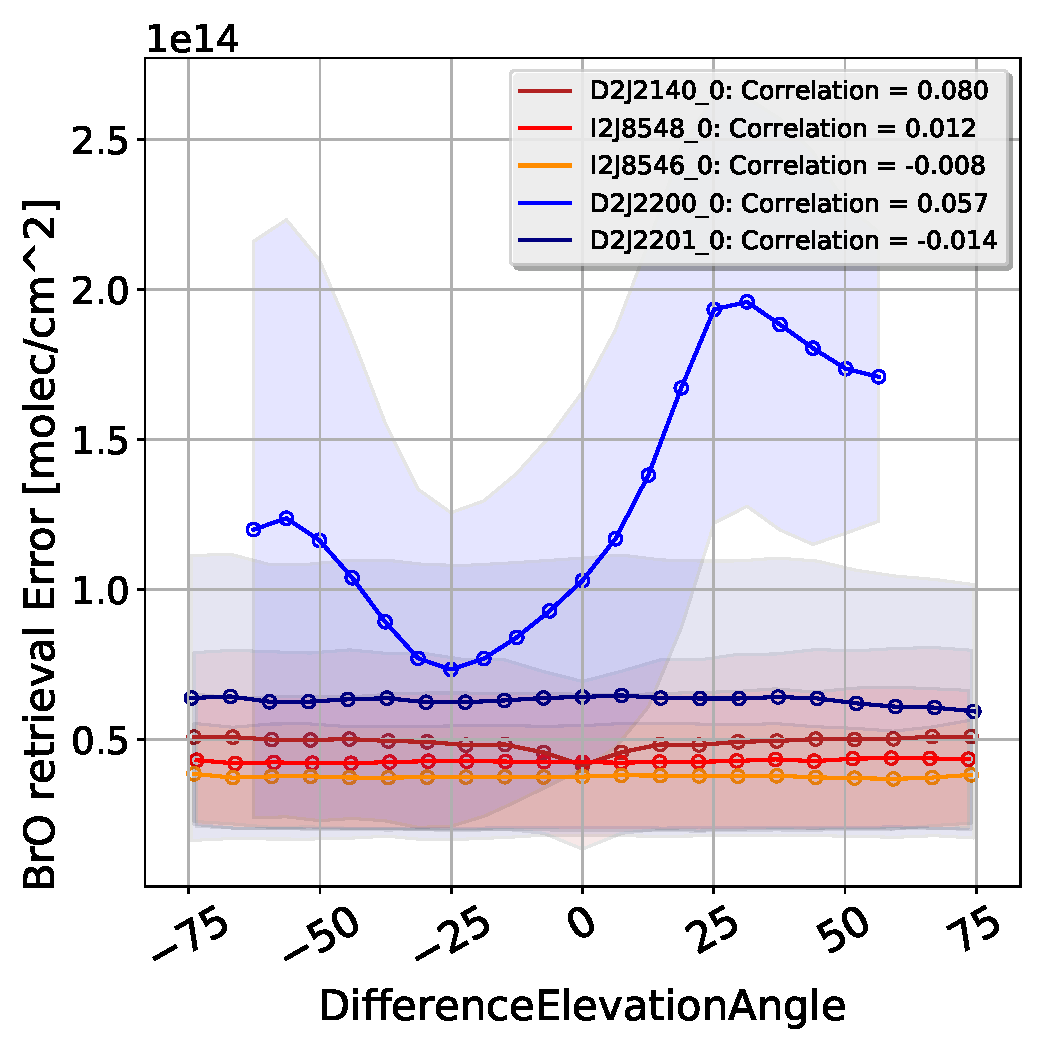
\includegraphics[width=0.7\linewidth]{Bilder/DiffElevAngleallInstruments}
	\caption{The \ce{BrO} measurement error as a function of the difference of elevation angle between the reference and the plume is shown for each of the individual instruments at Tungurahua and Nevado del Ruiz. To evaluate the plume spectra all reference spectra with a temporal distance of no longer than two weeks are used. The plots do not reveal a symmetry around axis with zero elevation angle difference for all instruments. The D2J2200 instrument at Nevado del Ruiz is not symmetric around zero.}
	\label{fig:diffeleangle}
\end{figure}
% tab_fit CAPTION
\begin{table}[h]
	\centering
	\begin{tabular}{|p{2cm}|p{2cm}|p{2cm}|p{2cm}|p{2cm}|p{2cm}|}
		%	\toprule
		Instrument	&D2J2140&I2J8546& I2J8548&D2J2200&D2J2201\\
		\toprule
		Slope& 1.73$\cdot$ e+8& 1.55$\cdot$ e+10  &-9.00$\cdot$ e+9 &2.92$\cdot$ e+11&-3.96$\cdot$ e+10\\
		\midrule
		Correlation&
		0.000&
		-0.010&
		0.012&
		0.065&
		-0.034\\
		\midrule
		Intercept&4.77$\cdot$ e+13&4.23$\cdot$ e+13&3.78$\cdot$ e+13&8.37$\cdot$ e+13 &6.44$\cdot$ e+13 \\
		\bottomrule
	\end{tabular}
	\caption{The \ce{BrO} measurement error as a function of the difference of elevation angle between the reference and the plume is fitted with a first order polynomial for each of the individual instruments at Tungurahua and Nevado del Ruiz. This table shows the fitting parameters slope and intercept. Moreover, the correlation between the \ce{BrO} error and the absolute elevation angle difference is shown. }
\end{table}
% same daytime / temperature plot 
%\begin{figure}
%	\subfigure{
%		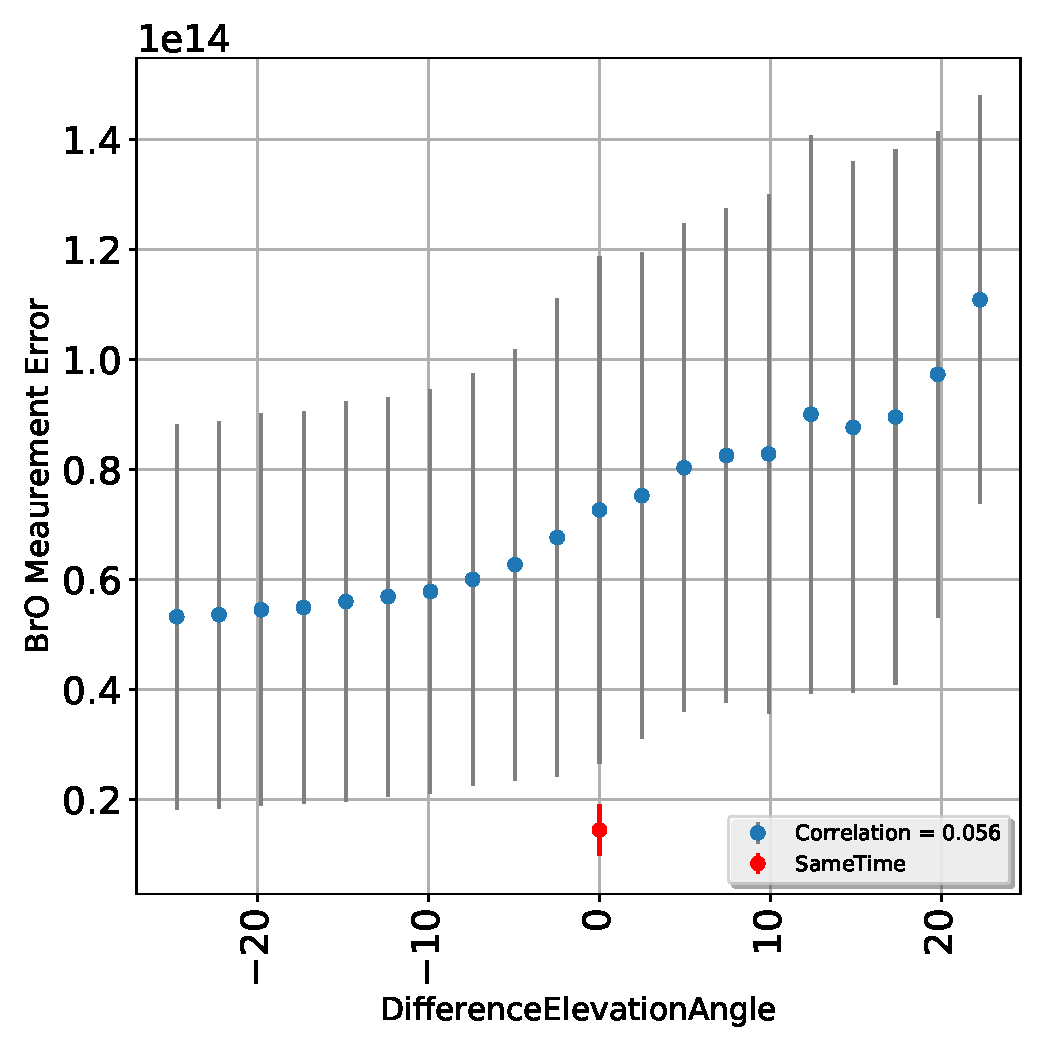
\includegraphics[width=0.49\linewidth]{Bilder/D2J2200_0_DiffElevAngle_onedaytime_Nevad}}
%	\subfigure{
%		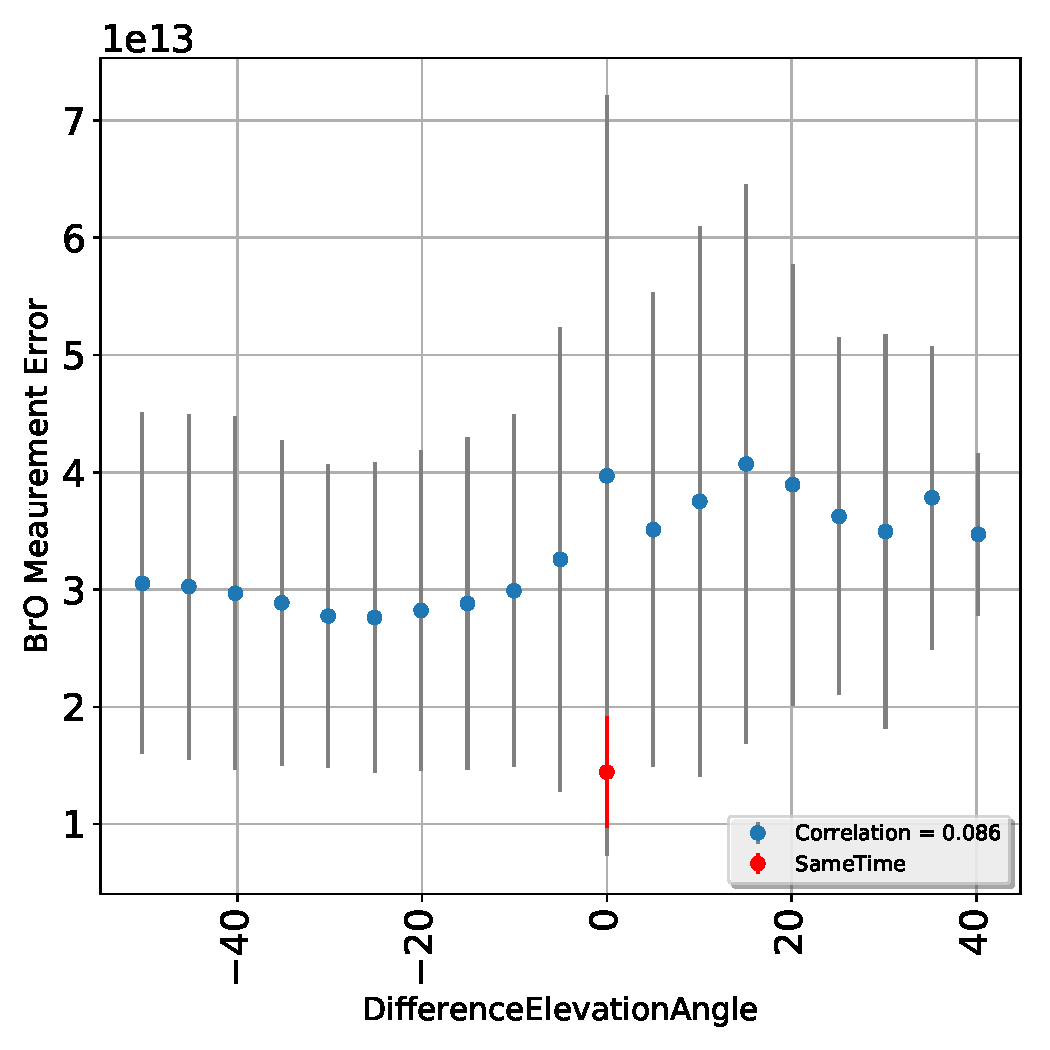
\includegraphics[width=0.49\linewidth]{Bilder/D2J2200_0_DiffElevAngle_onetemp_Nevad}}
%	\caption{The BrO measurement error as a function of the difference of elevation angle between the reference and the plumefor the D2J2200 instrument. Left: restricted to a constant difference in daytime (difference of $\pm 1h$), right: restricted to a constant difference in temperature (difference of $\pm 1^\circ$C).}
%	\label{fig:d2j22000diffelevangleonetempnevad}
%\end{figure}
\begin{figure}
	\centering
	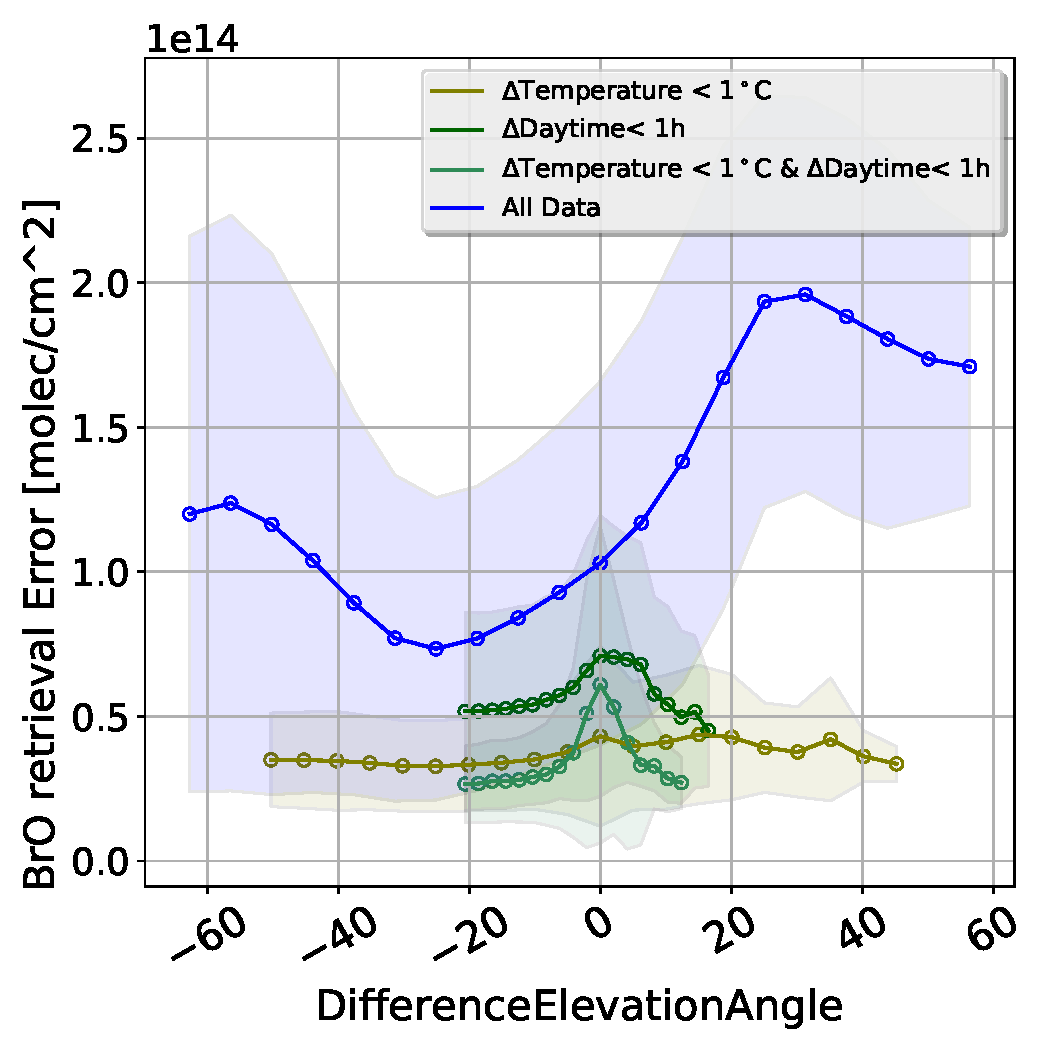
\includegraphics[width=0.7\linewidth]{Bilder/DiffElevAngleKomischesInstr}
	\caption{The \ce{BrO} measurement error as a function of the difference of elevation angle between the reference and the plume for the D2J2200 instrument. To evaluate the origin of the behavior of the \ce{BrO} retrieval error of the D2J2200 instrument as a function of the difference in elevation angle, the data are analysed on its temperature and daytime dependence. The same dependence is shown with restriction to an difference in temperature ($\Delta$Temperature) of below 1$^{\circ}C$ or restriction on a daytime difference of below 1h ($\Delta Daytime \pm 1h$). The curves are marked with different green color tones, as it is shown in the legend. The blue line shows the \ce{BrO} error as function of the elevation angle, when using all data for comprehension.}
	\label{fig:d2j22000diffelevangleonetempnevad}
\end{figure}


The elevation angle describes the angle between the horizon and the zenith. When using the plume spectrum and the reference spectrum of the same time, the difference in elevation angle cannot be zero, since the location of the plume does not coincidence with the location of the reference.\\
In \cref{fig:diffeleangle} the \ce{BrO} error is plotted as a function of the elevation angle. No significant correlation between the two parameters can be identified. \\
Only the data of the D2J2200 instrument significantly vary with the elevation angle. The observable variation of the \ce{BrO} error with the elevation angle differs from the symmetric dependence of all other external parameter, the minimum \ce{BrO} error can be found at a difference in elevation angle of -20$^{\circ}$. This curve is a result of the solar altitude over the day which can be obtained if only using data of the same day time. Such a plot can be seen in \Cref{fig:d2j22000diffelevangleonetempnevad}.
\Cref{fig:d2j22000diffelevangleonetempnevad} shows the \ce{BrO} retrieval error as function of the difference elevation angle for the D2J2200 instrument at the Nevado del Ruiz volcano. The blue line is equivalent to the results which are shown in \Cref{fig:diffeleangle} for comparison. The green lines show data, with a maximal difference in temperature of 1$^{\circ}C$ or maximal difference in daytime of 1$h$. If restricting the data to just small differences in temperature or/and daytime, the dependency between the \ce{BrO} retrieval and elevation angle appears to be not significant. Whereas the maximum of the \ce{BrO} error can be found at an difference in elevation angle of zero.\\
\\	
Since the \ce{BrO} error does not depend significantly on the elevation angle no restriction on difference of the elevation angle is needed.
\subsection{Exposure time}
\begin{figure}
	\centering
	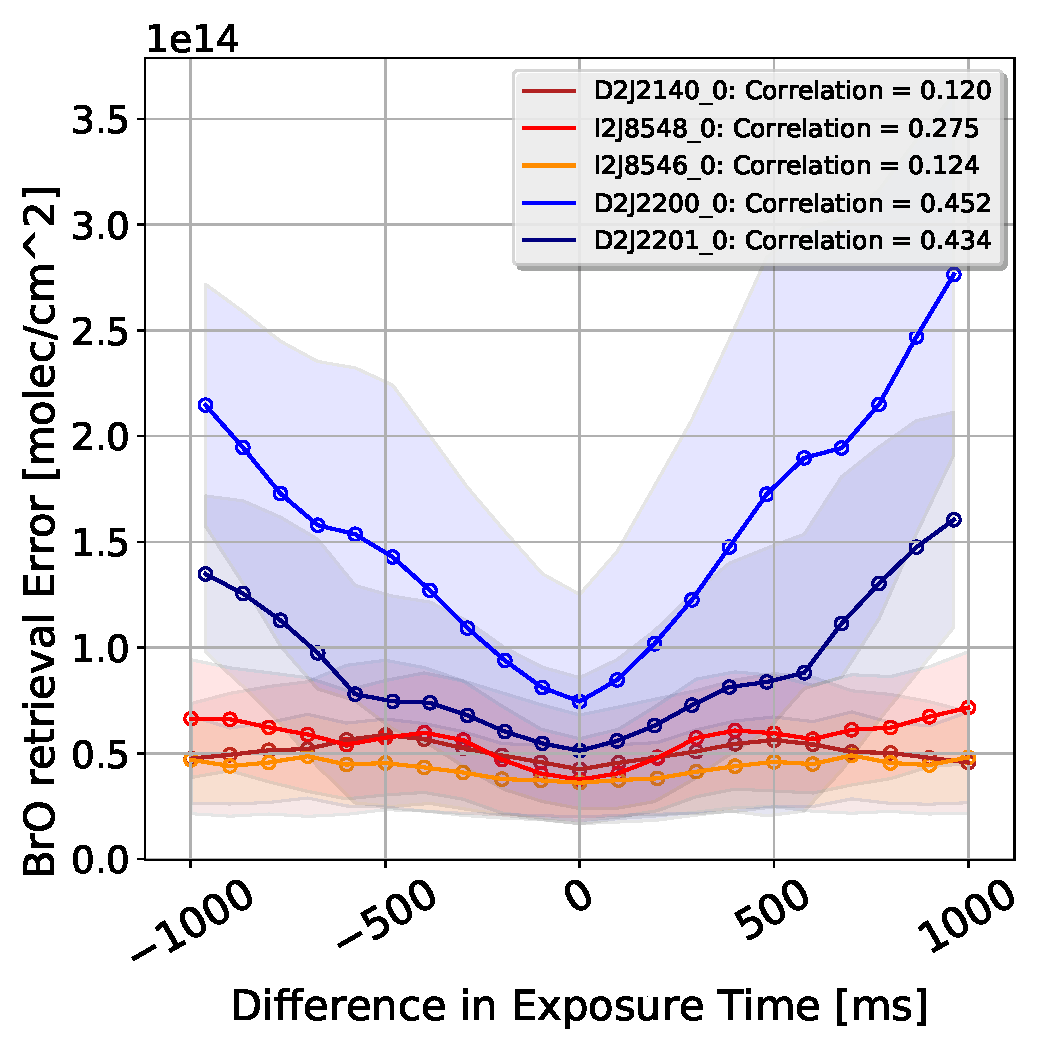
\includegraphics[width=0.7\linewidth]{Bilder/DiffExpTimeallInstruments}
	\caption{The \ce{BrO}  measurement error as a function of the difference of exposure time between measuring the reference and the plume are shown. To evaluate the plume spectra all reference spectra with a temporal distance of no longer than two weeks are used. An increase of the \ce{BrO} error with the distance in exposure time is observable.}
	\label{fig:diffexptime}
\end{figure}
The  exposure time is the length of time the sensor of the NOVAC instrument is exposed to light. In one scan the exposure time is set constant to the exposure time of the first scan, the pre-reference. The amount of light that reaches the film or image sensor is proportional to the exposure time. The exposure time is adjusted in the way that the maximum intensity does not overly the capacity of the sensor. Thus, the exposure time can be used as a degree of sky lightness.\\
We can observe a small dependency of the \ce{BrO} error on the exposure time at Tungurahua and Nevado del Ruiz as it is shown in \Cref{fig:diffexptime}. The \ce{BrO}  error as a function of the difference in exposure time is also symmetric around zero for all instruments. Thus the absolute difference in the exposure time is sufficient for the evaluation.\\
The instruments at Tungurahua do not show a significant dependence (correlation coefficient between 0.067 and 0.251) on the exposure time, even though there is always a minimum of the \ce{BrO} error at a difference of the Exposure Time of 0ms.\\
Nevado del Ruiz shows a stronger correlation between the \ce{BrO}  error and the exposure time.
\begin{table}[h]
	\centering
	\begin{tabular}{|p{2cm}|p{2cm}|p{2cm}|p{2cm}|p{2cm}|p{2cm}|}
		%	\toprule
		Instrument	&D2J2140&I2J8546& I2J8548&D2J2200&D2J2201\\
		\toprule
		Slope& 5.54$\cdot$ e+9&1.54$\cdot$ e+10 &3.04$\cdot$ e+10&1.72$\cdot$ e+11&9.37$\cdot$ e+10\\
		\midrule
		Correlation&0.067
		&0.121&
		0.251&
		0.452&
		0.434\\
		\midrule
		Intercept&4.63$\cdot$ e+13&3.58$\cdot$ e+13& 3.87$\cdot$ e+13& 6.88$\cdot$ e+13& 4.68$\cdot$ e+13\\
		\midrule
		$\Delta T_{2}$&8357&662&1273&95&499\\
		\bottomrule
	\end{tabular}
	\caption{The \ce{BrO} measurement error as a function of the difference of exposure time between the reference and the plume is fitted with a first order polynomial for each of the individual instruments at Tungurahua and Nevado del Ruiz. This table shows the fitting parameters slope and intercept. Moreover, the correlation between the \ce{BrO} error and the absolute exposure time difference is shown.}
	\label{tab:exptimecalc}
\end{table}

\begin{table}
	\centering
	\begin{tabular}{|p{1.8cm}|p{2.15cm}|p{2.15cm}|p{2.15cm}|p{2.15cm}|p{2.15cm}|}
		%	\toprule
		Instrument	&D2J2140&I2J8546& I2J8548&D2J2200&D2J2201\\
		\toprule
		Mean&
		81.7 ($\entspricht\,$96.5\%)		&162.8 ($\entspricht\,$99.4\%)		&212.8 ($\entspricht\,$98.0\%)		&284.0 ($\entspricht\,$100\%)		&225.6 ($\entspricht\,$100\%) \\
		\midrule
		Std&
		35.3 ($\entspricht\,$98.6\%)&		30.1 ($\entspricht\,$101\%)&
		64.5 ($\entspricht\,$99.5\%) &		69.5 ($\entspricht\,$100\%) &
		41.2 ($\entspricht\,$100\%) \\
		\midrule
		Min  &
		8 $\qquad$($\entspricht\,$100\%)&113 ($\entspricht\,$100\%)
		&95 ($\entspricht\,$97.9\%)
		&64 ($\entspricht\,$100\%)
		&63 ($\entspricht\,$100\%)\\
		\midrule
		Max&
		167 ($\entspricht\,$98.8\%) &
		214 ($\entspricht\,$100\%) &
		395 ($\entspricht\,$99.0\%) &
		433 ($\entspricht\,$100\%)  &
		297 ($\entspricht\,$100\%) \\
		\bottomrule
	\end{tabular}
	\caption{Amount of possible references when restricting the difference in exposure time  between plume and reference to differences below 632.25 ms.}
	\label{tab:etrest}
\end{table}	


\Cref{tab:exptimecalc} shows the slope, correlation, intercept and the $\Delta ET_{2}$s. The differences in exposure time where the \ce{BrO} error increases by a factor of two compared to the difference of exposure time of zero.
Restrictions of the exposure time to the mean of the $\Delta ET_{2}$s of all instruments which is 632.25 ms leads to an average decrease compared to \cref{Tab:refstime} of data of 98.78\%. The results for each instrument can be found in \cref{tab:etrest}.\\
\\
\\
\begin{table}
	\centering
	\begin{tabular}{|p{1.8cm}|p{2.15cm}|p{2.15cm}|p{2.15cm}|p{2.15cm}|p{2.15cm}|}
		%	\toprule
		Instrument	&D2J2140&I2J8546& I2J8548&D2J2200&D2J2201\\
		\toprule
		Mean&
		36.0 ($\entspricht\,$42.6\%)&	112.9 ($\entspricht\,$69.0\%)&
		148.9 ($\entspricht\,$68.6\%)&	217.0 ($\entspricht\,$76.4\%)&	140.4 ($\entspricht\,$62.2\%)\\
		\midrule
		Std&
		22.35 ($\entspricht\,$62.4\%)&
		50.6 ($\entspricht\,$169.2\%) &
		75.9 ($\entspricht\,$117.1\%)&
		82.1 ($\entspricht\,$118.1\%) &
		71.0 ($\entspricht\,$172.3\%) \\
		\midrule
		Min&
		1$\qquad$ ($\entspricht\,$12.5\%)  &
		8$\qquad$ ($\entspricht\,$7.1\%)  &
		12 ($\entspricht\,$12.4\%)  &
		3$\qquad$ ($\entspricht\,$4.7\%)   &
		6$\qquad$ ($\entspricht\,$9.5\%)  \\
		\midrule
		Max
		&127 ($\entspricht\,$75.1\%)
		&212 ($\entspricht\,$99.1\%)
		&382 ($\entspricht\,$95.7\%)
		&398 ($\entspricht\,$91.9\%)
		&283 ($\entspricht\,$95.3\%)\\
		\bottomrule
	\end{tabular}
	\label{tab:restrictall}
	\caption{Amount of possible references while restricting the difference in colorindex  between plume and reference to differences above 0.255. maximal Time difference is 3.358$^{\circ}C$, maximal daytime difference is 4.75h without Exposure Time  between plume and reference to differences below 632.25 ms.}
\end{table}	
\Cref{tab:restrictall} shows the amount of possible references if the only data are considered which do not exceed the thresholds in each external parameter.  The average amount of available references per plume decreases to 64\%. While the performance is as good as without the restriction, this means the averaged BrO error is almost the same (deviations are below 0.1\%).



	\subsection*{Dependence of external parameters on each other}
	In all discussions on the impact of the external parameter on the retrieved \ce{BrO}  error the  dependency of the external parameter on each other are neglected. It is plausible that the temperature correlates with the cloudiness or the lightness due to sunlight. Therefore the correlation of the exposure time with the \ce{BrO}  error could be a result of the correlation of the temperature with the \ce{BrO}  error. \Cref{fig:difference-in-exposure-time-msdifference-in-temperature-ctungu} shows an example of the dependency of external parameters on each other. The difference in temperature as a function of the difference in exposure time. The \ce{BrO}  error is color-coded. \\
	All correlations between the external parameters are shown in \Cref{fig:varcorrelationmatrix}. \Cref{fig:varcorrelationmatrix} shows discrete correlation values from 0.3 to 1. Correlations below 0.3 are ignored. Small plus and minus signs indicate whether the correlation is negative or positive. 
	The temperature depends on the daytime, due to the dependence of the temperature on the sun, thus a correlation between the  difference in temperature and the difference in daytime (correlation of $\approx$ 0.5) can be observed. Since the temperature depends on the intensity of the sun, it also correlates with  the difference in exposure time (correlation of $\approx$ 0.4). The difference in temperature also slightly correlates with the difference in colour index, due to the dependency of temperature on the cloudiness (correlation of $\approx$ 0.3). The low correlations could appear due to the uniform cloudiness near to the equator. The correlation between the temperature difference to the temporal difference (correlation of $\approx$ 0.3) probably occurs due to long term changes in temperature. Furthermore the difference in exposure time correlates with the daytime and the colour index (correlation of $\approx$ 0.4) as a result of the dependency on the sun intensity.\\
	\begin{figure}[h]
		\centering
		\includegraphics[width=0.7\linewidth]{"../Ausarbeitung/Uebersicht/Bilder/Difference in Exposure Time [ms]_Difference in Temperature [C]_Tungu"}
		\caption{An example of the dependency of external parameters on each other. The difference in temperature as a function of the exposure time. Data from Tungurahua.}
		\label{fig:difference-in-exposure-time-msdifference-in-temperature-ctungu}
	\end{figure}
	\begin{figure}[h]
		\centering
		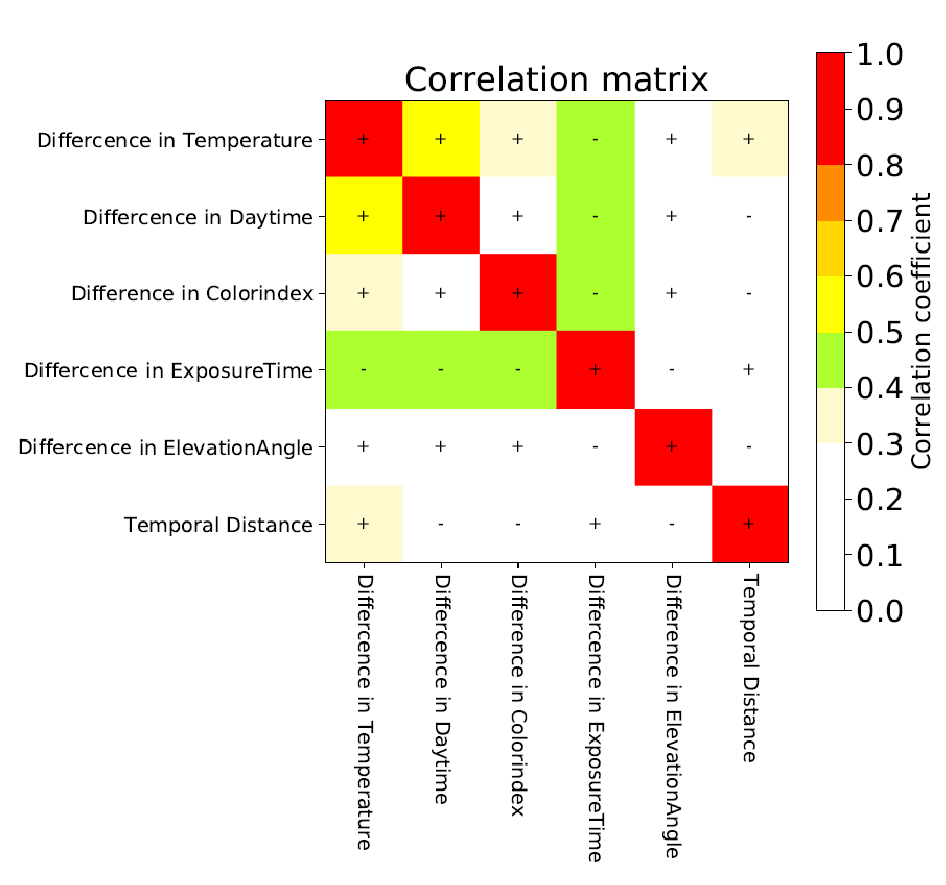
\includegraphics[width=1\linewidth]{Bilder/varCorrelation_matrix}
		\caption[Correlation matrix of the external parameters using the data from D2J2140\_0.]{Correlation matrix of the external parameters. The correlation is discrete colour coded. Positive correlation is labeled with a plus whereas negative correlation is labeled with a minus. The correlation matrix is calculated using the data from D2J2140\_0.}
		\label{fig:varcorrelationmatrix}
	\end{figure}
%
	To eliminate the correlation between the external parameters the \ce{BrO}  error dependency on one external parameter where calculated by keeping the differences in the other external parameters constant. Hereby only parameters were kept constant, where the correlation is above 0.3. Thus, when looking at the daytime, only the difference in temperature and exposure time need to be constant, since the daytime  difference does not correlate with the other considered external parameter. The results can be seen in \cref{fig:datwithoutotherparamallinstruments} to \cref{fig:diffdaytimewithoutotherparamallinstruments}.\\
	\\
	\Cref{fig:datwithoutotherparamallinstruments} shows the BrO retrieval error as a function of the temporal difference between the reference and the plume spectrum. All differences in temperature are below one degree. Compared to the correlations, calculated without eliminating the dependence on the temperature, the correlations increase. The dependence of the instruments installed at Tungurahua are still significant higher. From the results can be interpreted that the temporal difference between the time when measuring the plume and the reference has a impact on the fit quality, but this impact is smaller as the impact of the instrument temperature.\\
	\Cref{fig:diffdaytimewithoutotherparamallinstruments} shows the BrO retrieval error as a function of the difference in daytime for all considered instruments. As it can be seen in \cref{fig:varcorrelationmatrix} the exposure time and the temperature need to be kept constant. The difference in temperature is below 1 degree, the difference in exposure time below 100 ms. A general decrease of the correlations compared to \cref{fig:diffdaytime} is observable.\\
 %
	\Cref{fig:diffcolidxwithoutotherparamallinstruments} shows the BrO retrieval error as a function of the difference in colour index for all instruments. The temperature and the exposure time shows a dependency on the colour index as it can be seen in \cref{fig:varcorrelationmatrix}. Both are kept constant, the difference in temperature is below 1 degree and the difference in exposure time is below 100 ms. The correlations decrease compared to \cref{fig:diffcolidx}. Especially the correlation of the D2J2201\_0 instrument decreases from 0.359 to 0.068.\\
	%
	\Cref{fig:diffexptimewithoutotherparamallinstruments} shows the dependency of the BrO retrieval error on the difference in exposure time for all considered instruments. Hereby, only data are used, where the difference in temperature is below 1 degree, the difference in colour index is below 0.05 and the difference in daytime is below one hour. The temporal difference and the difference in elevation angle are not kept constant, since one could not observe a relation between the exposure time and the temporal difference or the elevation angle. The correlations between the BrO fit error and the difference in exposure time decrease for each instrument if the temperature, daytime and colour index are kept constant. Even though, the correlations at Nevado del Ruiz are still higher as the correlations at Tungurahua.\\
	Restricting the data, to where the temperature difference is kept below one degree, leads to an distortion of the data. Thus the results plotted in \cref{fig:datwithoutotherparamallinstruments} to \cref{fig:diffdaytimewithoutotherparamallinstruments} could also have systematic errors.\\
	When comparing the correlations of the data from \cref{fig:datwithoutotherparamallinstruments} and \cref{fig:diffexptimewithoutotherparamallinstruments}  to the correlations of 
	\cref{fig:datallinstruments} to \cref{fig:diffexptime} a large reduction of the correlation is obvious. Only the difference in temperature still shows a significant correlation to the \ce{BrO}  error. However, the minimal \ce{BrO}  error coincidence in almost all cases with a difference in external parameters of zero. A dependency of the \ce{BrO}  error on the external parameter can still be seen even tough the correlation is very small. \\
	Excluding of the external parameters due to the rather low correlation leads to a worse quality of the results, since the effects of the single parameter add up to a not negligible amount. However, note that  the added impact of all external parameter except for the temperature are less important than the temperature.
	The BrO fit error of contaminated spectra evaluated with the new method in the following refereed to as decontamination module (See \cref{chapt:contbased}) increases by 15\% if the other external parameters are excluded. If all external paramter except for the temperature are used the calculated BrO fit error increases by 37\%.\\
	\\
	For the final evaluation of contaminated data I use the results of \cref{fig:difftemp} to \cref{fig:diffcolidx}. Since the correlations between the external parameters are considered in the final 4 dimensional fit.\\
	\begin{figure}[h]
		\centering
		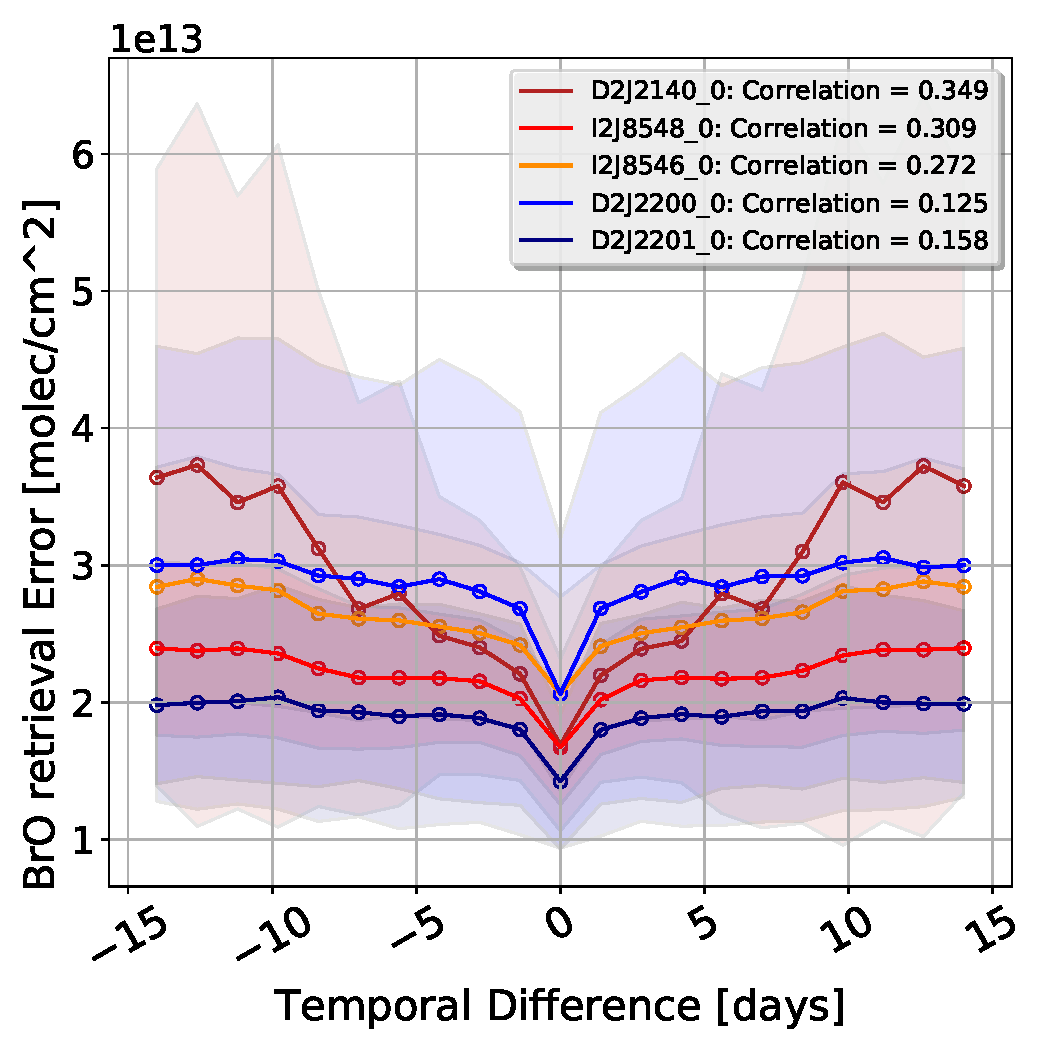
\includegraphics[width=0.5\linewidth]{Bilder/BrOErr_OhnEVar/DatwithoutOtherparamallInstruments}
		\caption{The BrO measurement error as a function of the temporal difference between measuring the reference and the plume are shown. Therefore, the reference spectra are restricted such that the maximal temperature difference between reference and plume is $1^\circ$ C.}
		\label{fig:datwithoutotherparamallinstruments}
	\end{figure}
\begin{figure}[h]
	\centering
	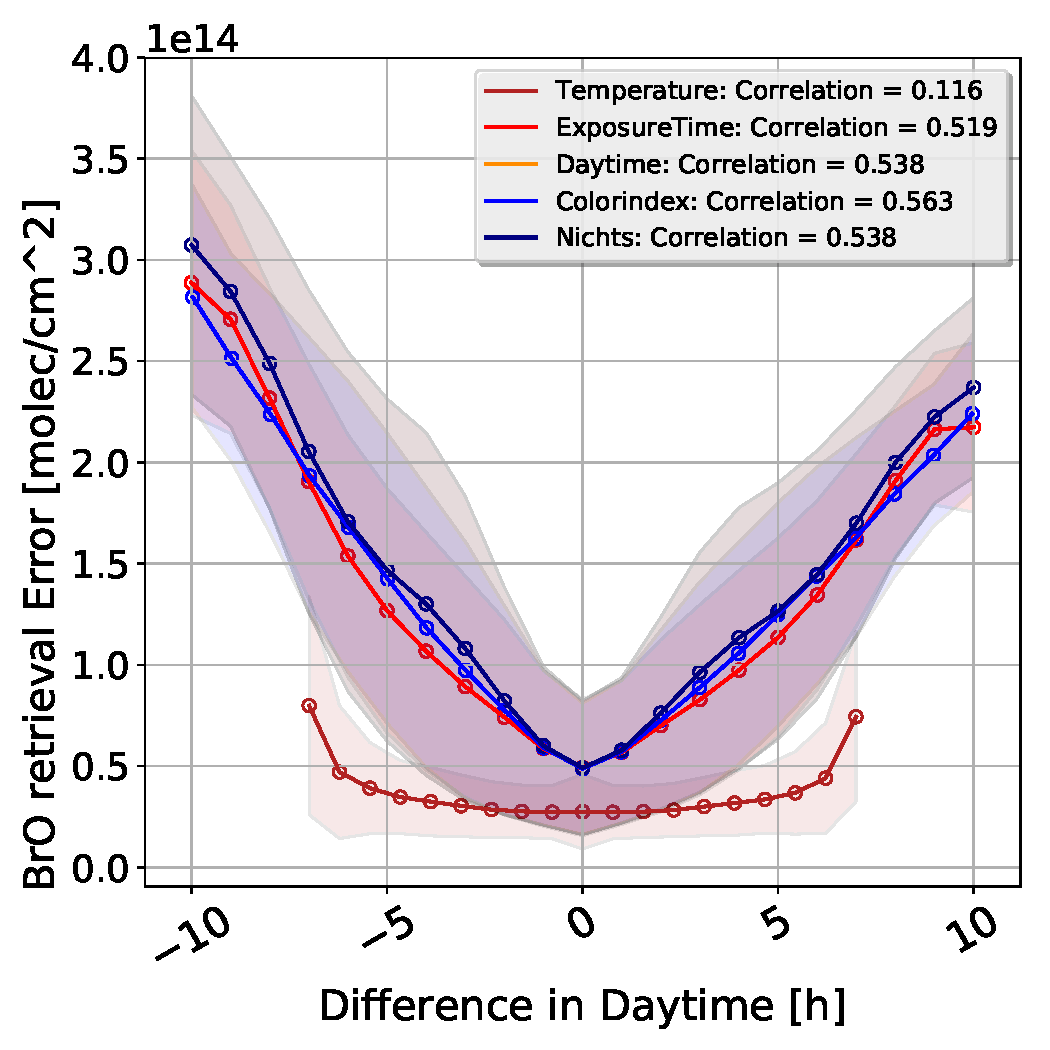
\includegraphics[width=0.5\linewidth]{Bilder/BrOErr_OhnEVar/DiffDaytimewithoutOtherparamallInstruments}
	\caption{The BrO measurement error as a function of the daytime difference between recording the reference and the plume are shown. Therefore, the reference spectra are restricted such that the maximal temperature difference between reference and plume is $1^\circ $C. The maximal exposure time difference is $100 $ms.
	}
	\label{fig:diffdaytimewithoutotherparamallinstruments}
\end{figure}
\begin{figure}[h]
	\centering
	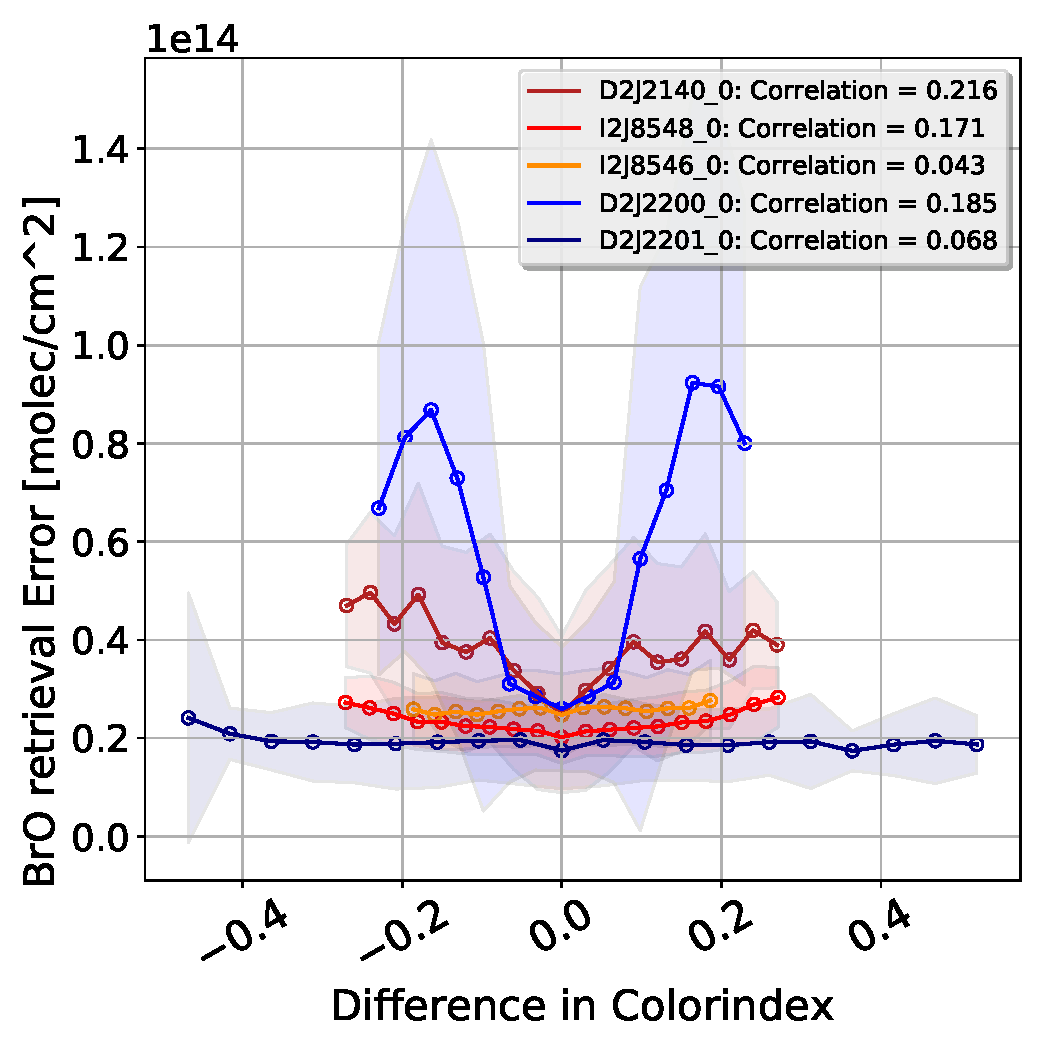
\includegraphics[width=0.5\linewidth]{Bilder/BrOErr_OhnEVar/DiffColidxwithoutOtherparamallInstruments}
	\caption{The BrO measurement error as a function of the color index difference between recording the reference and the plume are shown. Therefore, the reference spectra are restricted such that the maximal temperature difference between reference and plume is $1^\circ $C. The maximal exposure time difference is $100 $ms.}
	\label{fig:diffcolidxwithoutotherparamallinstruments}
\end{figure}
\begin{figure}[h]
	\centering
	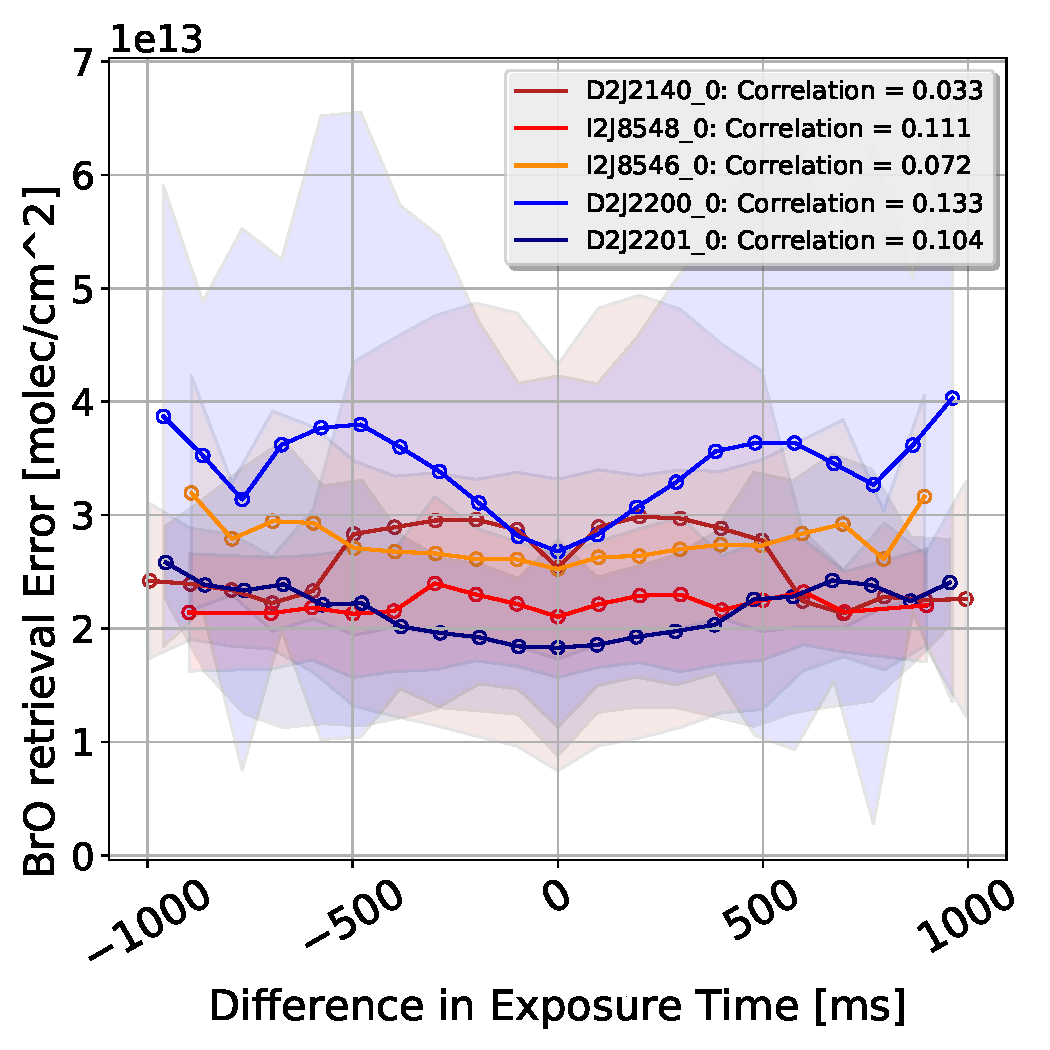
\includegraphics[width=0.5\linewidth]{Bilder/BrOErr_OhnEVar/DiffExpTimewithoutOtherparamallInstruments}
	\caption{The BrO measurement error as a function of the exposure time difference between recording the reference and the plume are shown. Therefore, the reference spectra are restricted such that the maximal color index difference between reference and plume is $0.05$. The maximal daytime difference is $1$h.}
	\label{fig:diffexptimewithoutotherparamallinstruments}
\end{figure}




	
%	\begin{figure}
%			\subfigure{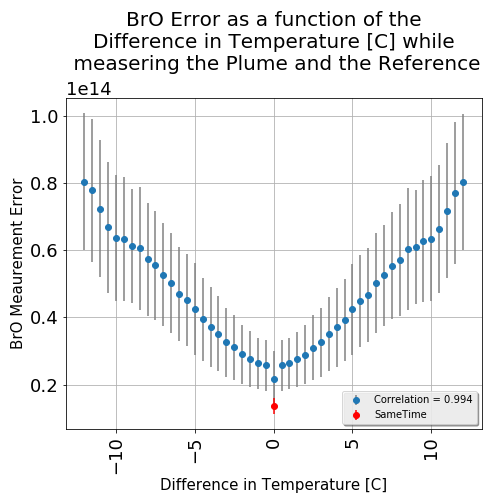
\includegraphics[width=0.3\linewidth]{Bilder/BrOError_onVariables_050218/I2J8546_0DiffTemp_Tungu}}
%			\subfigure{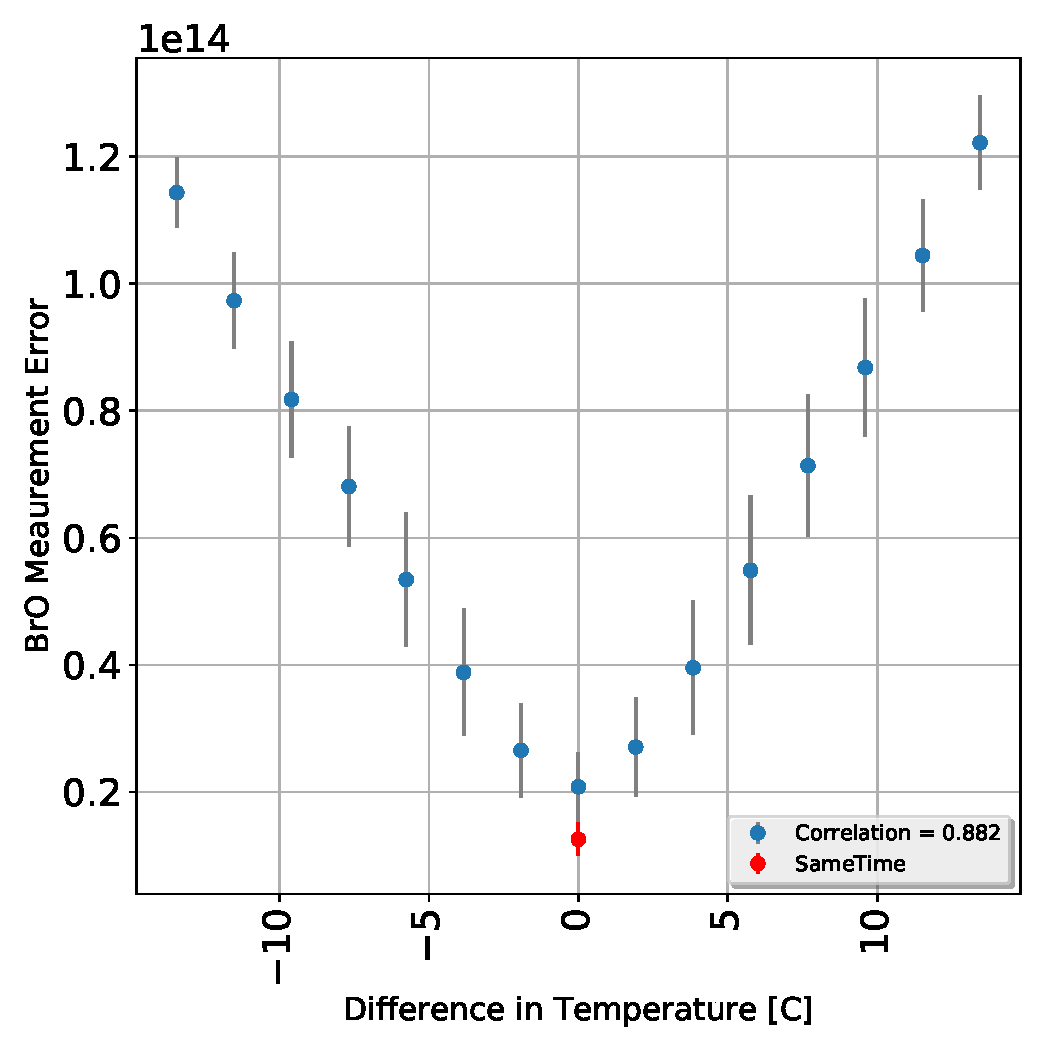
\includegraphics[width=0.3\linewidth]{Bilder/BrOError_onVariables_050218/I2J8548_0DiffTemp_Tungu}}
%			\subfigure{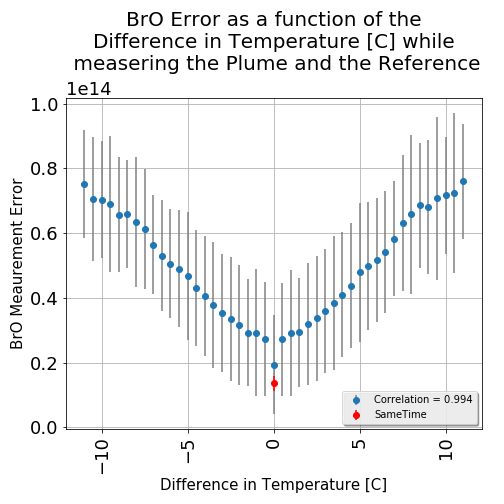
\includegraphics[width=0.3\linewidth]{Bilder/BrOError_onVariables_050218/D2J2140_0DiffTemp_Tungu}}
%		\subfigure{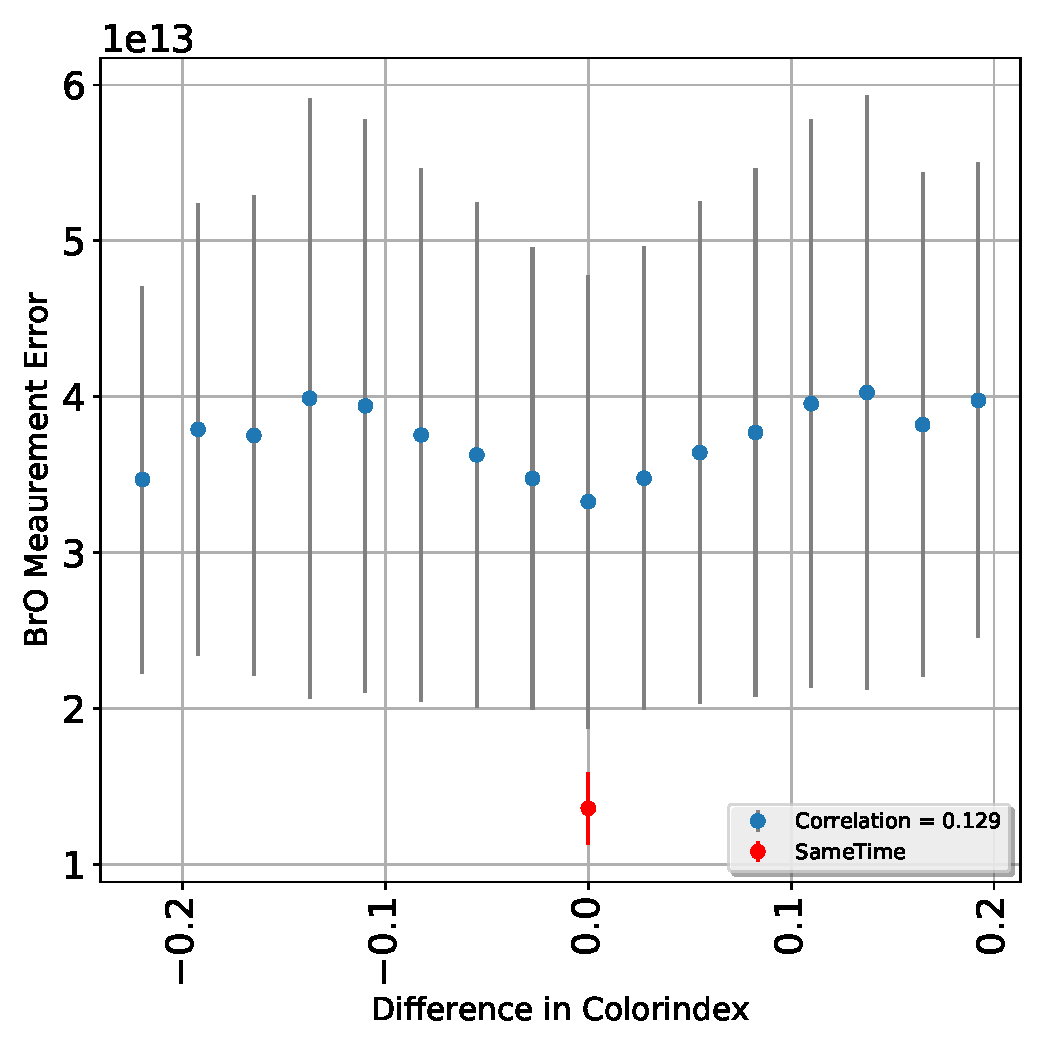
\includegraphics[width=0.3\linewidth]{Bilder/BrOError_onVariables_050218/I2J8546_0DiffColidx_Tungu}}
%		\subfigure{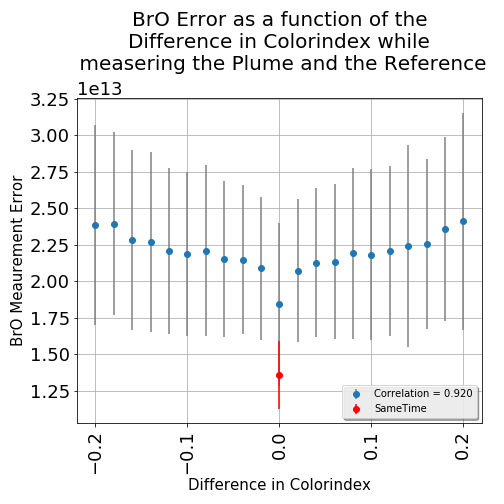
\includegraphics[width=0.3\linewidth]{Bilder/BrOError_onVariables_050218/I2J8548_0DiffColidx_Tungu}}
%		\subfigure{\includegraphics[width=0.3\linewidth]{Bilder/BrOError_onVariables_050218/D2J2140_0DiffColidx_Tungu}}
%
%		\subfigure{\includegraphics[width=0.3\linewidth]{Bilder/BrOError_onVariables_050218/I2J8546_0DiffDaytime_Tungu}}
%		\subfigure{\includegraphics[width=0.3\linewidth]{Bilder/BrOError_onVariables_050218/I2J8548_0DiffDaytime_Tungu}}
%		\subfigure{\includegraphics[width=0.3\linewidth]{Bilder/BrOError_onVariables_050218/D2J2140_0DiffDaytime_Tungu}}
%
%		\subfigure[I2J8546\_0]{\includegraphics[width=0.3\linewidth]{Bilder/BrOError_onVariables_050218/I2J8546_0DiffExpTime_Tungu}}
%		\subfigure[I2J8548\_0]{\includegraphics[width=0.3\linewidth]{Bilder/BrOError_onVariables_050218/I2J8548_0DiffExpTime_Tungu}}
%		\subfigure[D2J2140\_0]{\includegraphics[width=0.3\linewidth]{Bilder/BrOError_onVariables_050218/D2J2140_0DiffExpTime_Tungu}}
%		\caption{DiffExpTime at Tungurahua}
%		\label{fig:DiffExpTime}
%	\end{figure}
%
%
%		\begin{figure}
%			\centering
%			\caption{\ce{BrO} error as a function of the external while measering the Plume and the Reference at Nevado del ruiz}
%			\subfigure{\includegraphics[width=0.3\linewidth]{Bilder/BrOError_onVariables_050218/D2J2201_0DiffTemp_Nevad}}
%			\subfigure{\includegraphics[width=0.3\linewidth]{Bilder/BrOError_onVariables_050218/D2J2200_0_DiffTemp_Nevad}}\\
%
%			\centering
%			\subfigure{\includegraphics[width=0.3\linewidth]{Bilder/BrOError_onVariables_050218/D2J2201_0DiffColidx_Nevad.pdf}}
%			\subfigure{\includegraphics[width=0.3\linewidth]{Bilder/BrOError_onVariables_050218/D2J2200_0_DiffColidx_Nevad.pdf}}
%
%			\subfigure{\includegraphics[width=0.3\linewidth]{Bilder/BrOError_onVariables_050218/D2J2201_0DiffDaytime_Nevad}}
%			\subfigure{\includegraphics[width=0.3\linewidth]{Bilder/BrOError_onVariables_050218/D2J2200_0_DiffDaytime_Nevad}}\\
%			\subfigure[D2J2201\_0]{\includegraphics[width=0.3\linewidth]{Bilder/BrOError_onVariables_050218/D2J2201_0DiffExpTime_Nevad}}
%			\subfigure[D2J2200\_0]{\includegraphics[width=0.3\linewidth]{Bilder/BrOError_onVariables_050218/D2J2200_0_DiffExpTime_Nevad}}
%			\label{fig:DiffExpTimeNevad}
%		\end{figure}


	\section{\ce{BrO}  dependence on external parameters\label{Chap:BrOdep}}
	The external parameters not only influence the fit quality but also the evaluation of the gas amount. A high difference in certain external parameter could distort the calculated \ce{BrO}  column density. \Cref{fig:d2j2140060218difftemperature-cbro} shows the evaluation of one plume with respect to different references. The temporal difference between the references and the plume do not exceed two weeks. In theory it is expected that the choice of  the reference should not make a difference, therefore all BrO column densities resulting from the evaluation should be equivalent. But one can see a high variation if choosing different references. The variability of the BrO column density depends as well on the external parameters, when looking at the temperature dependency a mean decrease of th BrO column density with an increasing temperature can be observed.
		\begin{figure}
		\subfigure[]{
			\includegraphics[width=0.5\linewidth]{"Bilder/OnePlumeMoreRefs_plumedate_081203_1646/D2J2140_0_6_02_18_DiffTemperature [C]_BrO"}}
		\subfigure[]{\includegraphics[width=0.5\linewidth]{"Bilder/OnePlumeMoreRefs_plumedate_081203_1646/D2J2140_0_plumeat12Temperature [C]_BrO_TemporalDiff"}}	
		\caption[One plume is evaluated by using different references.  The y axis shows the \ce{BrO} SCD difference between the NOVAC routine and decontamination module. (a) The difference in \ce{BrO}  as a function of the temperature difference. (b) The difference in \ce{BrO} as a function of the temporal difference between the one plume and the different references.]{One plume is evaluated by using different references. The plume is recorded at Tungurahua volcano with the D2J2140\_0 instrument. The recording time was the  03.12.2008  at 16:46 o clock. The y axis shows the \ce{BrO}  column density difference between the NOVAC method and decontamination module. (a) The difference in \ce{BrO}  is plotted as a function of the temperature difference between the plume and the references. Every data point indicates one reference. (b) The difference in \ce{BrO}  is plotted as a function of the temporal difference between the one plume and the different references.}
		\label{fig:d2j2140060218difftemperature-cbro}		
	\end{figure}
	\Cref{fig:d2j2140060218difftemperature-cbro} is a result of an exemplary evaluation of one plume. An examination of all several plumes evaluated by different references is shown in \cref{fig:difftempbroallinstruments}. The plots are equivalent to the plots for BrO fit error (for an example see \cref{fig:difftemp}). The BrO SCDs vary strongly with the differences in external parameters. It is observable, that the BrO SCDs recorded by the instruments at Nevado del Ruiz vary in a larger range than for the BrO SCDs recorded by instruments at Tungurahua. This can also be observed for the BrO retrieval errors. The absolute BrO SCDs increase with the difference in external parameters.\\
	 \Cref{fig:difftempbroallinstruments} (a): Temporal difference: For the temporal difference no significant correlation can be observed.
	 %
	\Cref{fig:difftempbroallinstruments} (b): Difference in daytime: For the instruments at Nevado del Ruiz the BrO SCD correlates strongly with the difference in daytime. This can be a result of the dependence on the temperature, since the correlations are very similiar, only the correlations are a little bit stronger for the difference in temperature.
	\Cref{fig:difftempbroallinstruments} (c): Difference in temperature: For the instruments at Nevado del Ruiz the BrO SCD correlates strongly with the difference in temperature. The correlations from the instruments at Tungurahua vary very much from -0.696 (D2J2140\_0) to 0.198 (I2J8546).
	 %
	 \Cref{fig:difftempbroallinstruments} (d) Difference in color index: The correlations differ for every instrument even for instruments of the same volcano. The correlations vary from -0.368 to 0.46.
	 %
	 \Cref{fig:difftempbroallinstruments} (e) The strange dependence which can be seen between the BrO fit error and the difference in elevation angle for the D2J2200\_0 instrumnt can be seen in this plot as well. The other instruments do not show any correlation between the BrO SCD and the difference in elevation angle.
	 %
	 \Cref{fig:difftempbroallinstruments} (f) The correlations for the difference in exposure time are opposite to the correlations in daytime. 
%	\Cref{fig:onerefd2j2140060218difftemperature-cbro} shows the exemplary evaluation of different plumes by on reference. Here I assume different column densities, but this variability should be independent of the difference in the external parameters. But \Cref{fig:onerefd2j2140060218difftemperature-cbro} shows a clear dependence on the Temperature. The correlation for this example is -0.76, thus it can be concluded, that here is also an significant dependence. 

%	\begin{figure}
%		\subfigure[]{
%		\includegraphics[width=0.5\linewidth]{"Bilder/OneRefMorePlumes_refdate_081115_1337/D2J2140_0_onerefTemperature [C]_BrO_TemporalDiff"}}
%		\subfigure[]{
%		\includegraphics[width=0.5\linewidth]{"Bilder/OneRefMorePlumes_refdate_081115_1337/onerefD2J2140_0_6_02_18_DiffTemperature [C]_BrO"}}
%		\caption{One Reference is used to evaluated different Plume spectra. The reference was recorded at Tungurahua volcano with the D2J2140\_0 instrument. recording time was the 081115 at 1337 o clock. The y axis show the \ce{BrO}  column density. (a) The \ce{BrO}  is plotted as a function of the temporal difference between the one reference and the plumes  (b) The \ce{BrO}  is plotted as a function of the temperature difference between the plume and the references. Every data point stands for another plume evaluated with the same reference.}
%		\label{fig:onerefd2j2140060218difftemperature-cbro}
%	\end{figure}
%	\begin{figure}
%		\includegraphics[width=0.7\linewidth]{"Bilder/OneRefMorePlumes_refdate_081115_1337/onerefD2J2140_0_6_02_18_DiffDaytime (Plume)_BrO"}
%		\caption{The difference of BrO when performing the evaluation with The NOVAC Method minus the decontamination module as a function of the Daytime when measuring the plume. The recording time of the reference was 081115 at 1337 o clock}
%		\end{figure}
%	\begin{figure}
%		\subfigure[]{
%		\includegraphics[width=0.5\linewidth]{"Bilder/BrODependencies/AllDataCorrWithBrOElevation Angle [deg]_BrO"}
%		}
%		\subfigure[]{
%		\includegraphics[width=0.5\linewidth]{"Bilder/BrODependencies/AllDataCorrWithBrOExposure Time [ms]_BrO"}
%		}
%		\subfigure[]{
%		\includegraphics[width=0.5\linewidth]{"Bilder/BrODependencies/AllDataCorrWithBrOTemperature [C]_BrO"}
%		}
%		\subfigure[]{
%		\includegraphics[width=0.5\linewidth]{Bilder/BrODependencies/AllDataCorrWithBrOColorindex_BrO}
%		}
%		\subfigure[]{
%		\includegraphics[width=0.5\linewidth]{"Bilder/BrODependencies/AllDataCorrWithBrODaytime (Plume)_BrO"}}
%		\caption{The Dependence of the BrO evaluation on external parameter is shown. }
%		\label{fig:alldatacorrwithbrodaytime-plumebro}
%	\end{figure}
\begin{figure}
	
	\subfigure{(a)
	\includegraphics[width=0.45\linewidth]{Bilder/BrOVariables/DatBrOallInstruments}
}
\subfigure{(b)
	\includegraphics[width=0.45\linewidth]{Bilder/BrOVariables/DiffDaytimeBrOallInstruments}
}
\subfigure{(c)
	\includegraphics[width=0.45\linewidth]{Bilder/BrOVariables/DiffTempBrOallInstruments}}
\subfigure{(d)
	\includegraphics[width=0.45\linewidth]{Bilder/BrOVariables/DiffColidxBrOallInstruments}
}
\subfigure{(e)
	\includegraphics[width=0.45\linewidth]{Bilder/BrOVariables/DiffElevAngleBrOallInstruments}
}
\subfigure{(f)
	\includegraphics[width=0.45\linewidth]{Bilder/BrOVariables/DiffExpTimeBrOallInstruments}
}
\caption{The BrO SCD as a function of the difference of the external parameters between measuring the reference and the plume are shown.}
	\label{fig:difftempbroallinstruments}
\end{figure}
\FloatBarrier
	\subsection*{Summary}
This chapter examines the influence of external on the precision of the BrO evaluation. Hereby the following parameter are considered: 
temporal difference, temperature, daytime, colour index, elevation angle, exposure time.  The findings are based on the data of three instruments installed at the Tungurahua volcano and two instruments at the Nevado del Ruiz volcano. The maximal temporal difference between measuring the plume and the reference is set to 14 days to prevent large uncertainties in the BrO evaluation. Due to the mechanical influence on the instrument line function the temperature for all analysed instruments has the most significant impact on the BrO evaluation for all considered external parameters. The elevation angle does not seem to influence the evaluation for all examined instruments thus the elevation is excluded from the evaluation. The influence of the other external parameter change at every instrument. So a relatively strong impact of the exposure time can be seen at the D2J2201\_0 instrument at Nevado del Ruiz, while the exposure time does not seem to significantly influence the evaluation of the data from the  I2J8548\_0 at Tungurahua. 
	
	%--------------------------------------------------------------------------------------------------------------
	\part{Retrieval advances}
\chapter{Decontamination module \label{chapt:contbased}}
%\textcolor{red}{Soweit ich verstanden habe, haben die "Other Approaches" keine Relevanz für dein Ergebnis. Aber sie stören den Lesefluss. Ich würde sie in den Appendix schieben.}\\

	Based on the findings about the influence of external parameters on the \ce{BrO} error I propose an algorithm which is able to pick an appropriate volcanic-trace-gas free reference. The algorithm uses the dependencies found in \cref{Chap:BROErr} to find a sufficiently good matching reference.\\ 
	The first step is, to evaluate every reference with solar atlas spectrum, to check for contamination. A reference is classified as contaminated if the fit against the solar atlas spectrum yields an \ce{SO2} SCD above the plume limit ($2\cdot 10^{17}$).\\
	\\
	In the second step for each contaminated reference an alternative gas-free reference spectrum need to be found:
	\begin{figure}
		\centering
		\includegraphics[width=0.7\linewidth]{Bilder/Cont}
		\caption[Visualization of the decontamination module.]{Visualization of the decontamination module. A list of possible references is available, where the temporal difference between the plume and the reference is not longer than two weeks. For every possible reference, the estimated BrO fit error is calculated by considering the corresponding difference in important external parameters. The reference with the so calculated minima BrO fit error is used for the evaluation.}
		\label{fig:Cont}
	\end{figure}

	\begin{itemize}
		\item A list of possible references is created where all references are not contaminated and the temporal distance to the plume date is no longer than 14 days.
		\item For all possible references the differences in the external parameters are calculated with respect to the corresponding plume spectrum.
		\item The analysis of external parameters as described in \cref{Chap:BROErr} is used to estimate the \ce{BrO} error of all references
		\item The reference with the smallest estimated \ce{BrO} fit error is chosen as new reference
		\item  The plume spectra of the corresponding scan is evaluated with the new reference.
	\end{itemize}

	%
	$\epsilon_{0}$ is the \ce{BrO} error when evaluate the plume spectrum with the "same-time-reference".
	The assumption is, that the \ce{BrO} error $\epsilon_{BrO}$ can be described as the sum of $\epsilon_{0}$ and the deviation of $\epsilon_{BrO}$ with respect to all external parameters. It is limited by the precision of the NOVAC-instruments.
	\begin{equation}
		\epsilon_{BrO} =  \epsilon_{0}+\frac{d\epsilon}{dt}+\frac{d\epsilon}{d ^{\circ}}+\frac{d\epsilon}{dT}+\frac{d\epsilon}{dDt} +\frac{d\epsilon}{dc} + \text{further influences} 
	\end{equation}
	\begin{equation}
		\rightarrow \Delta \epsilon_{BrO} =\epsilon_{BrO} - \epsilon_{0} =\frac{d\epsilon}{dt}+\underbrace{\frac{d\epsilon}{d ^{\circ}}}_{=0}+\frac{d\epsilon}{dT}+\frac{d\epsilon}{dDt} +\frac{d\epsilon}{dc} + \text{further influences}
		\label{calc:err}
	\end{equation}
	Here the parameter $t$ stands for the time between plume-time and reference-time. The parameter $T$ is the difference in temperature. The parameters $Dt$ and $c$ are the differences in the daytime and the colour index.
	The task occurring at this stage is to find the best representation for the deviations. And then find the reference which minimize $\Delta \epsilon_{BrO} $\\
	%
	\\
	%
	The straight-forward way is to just calculate the \ce{BrO} error of all possible references for every plume by using the DOASIS routine. If this method is used it is possible to choose the reference for which the \ce{BrO} error is minimal. However this takes to much computation time since the evaluation time would be proportional to the number of possible references because the evaluation needs to be done for $\mathcal{O}(n)$ with $n$ as the number of potential reference spectra. Doing this evaluation for every plume-reference pair makes it impossible to do the evaluation in real, or near real time.
	Furthermore taking the minimum in all cases is statistically risky since the good results can occur accidental. The interpretation is thus more easy if the algorithm searches for an appropriate reference in a defined parameter range.\\
	%
	In this thesis a novel approach of identifying an ideal reference spectrum, by considering externel parameters, is introduced. This way a much faster estimation with constant complexity $\mathcal{O}(1)$ is reached.
	But the above described optimal evaluation is used to rate new approach and compare them among each other. The optimal evaluation always choose the reference with the smallest absolute error. We don't use the relative error due to its vulnerability. Using the relative error leads to less precision since the references with the highest BrO column density is preferred.\\
	%
	The results of the algorithm which chooses the reference automatically are described relative to an optimal evaluation. To avoid an distortion of the results due to relatively bad match between reference and plume spectra all data with a relative BrO fit error larger than one are excluded from the evaluation.\\
	\\
	In the following I examine several methods for choosing the best reference based on the analysis of external parameters. 
	
\section{Fit with a first order polynomial}
	The following chapter analyses fitting the data with a first order polynomial. \Cref{fig:difftemp} to \cref{fig:diffexptime} show the \ce{BrO}  error as a function of external parameters. Hereby, the curves are symmetric around zero difference in the respective external parameter. Therefore, it is not necessary to distinguish between positive or negative deviations from the equal surrounding conditions. Thus, the absolute differences can be utilized. Using the absolute difference leads to less complex calculations and therefore to a lower calculation time. On the other hand not using the absolute difference leads to no measurable advantages. \\
	\\
	%
	A linear approximation of the \ce{BrO}  error as function of the considered external parameters leads to a variation of  \cref{calc:err} :
	With linear differentiations of the \ce{BrO}  error with respect to the respective external parameters \cref{calc:err} can be written as:	
	\begin{equation}
		\Delta \epsilon_{BrO} = a_{t}\cdot\Delta t+a_{ET}\cdot\Delta ET+a_{T}\cdot\Delta T+a_{Dt}\cdot\Delta Dt +a_{c}\cdot\Delta c + \text{further influences}
		\label{calc:delterr}
	\end{equation}
	%
	To determine the coefficients $a_{x}$ (\cref{calc:delterr}) the data visualized in \cref{fig:difftemp}-\ref{fig:diffexptime} where used.  The fitting is done with an ordinary least square linear regression. In particular I used the python function linear regression from the library sklearn \citep{SKlearn}. \\
	
	As it can be seen in \cref{Chap:BROErr} the impact of the different external parameters change for every instrument depending on the location and the instrument themselves. 
	While the \ce{BrO}  error does not show any dependence on some external parameters for some instruments, the error has very strong dependence on the same external parameter at an other instrument. An example is the correlation between \ce{BrO}  error and the difference in daytime of 0.6 for D2J2201\_0 (Nevado del Ruiz) and a correlation of 0.16 for I2J8546\_0 (Tungurahua).
	To get a more stable algorithm less external parameter are preferable. Thus, it is necessary to distinguish between the stability of the fit, which improves with less external parameters and quality of the fit, which improves with more external parameters. 
	A preferable strategy is, to find a solution which is valid for all instruments. Moreover, utilizing less external parameters saves computation time.
	One possibility is to use all external parameters where the correlation is above a certain value. Since a selection valid for all instruments is preferred there are two possibilities: The first one is that one decide by using the mean correlation of all instruments. The second option is to use the highest correlation.
	
	\begin{table}[h]
		\centering
		\caption{The correlation coefficients between the BrO measurement error and the different external parameters. As a correlation value both the average and the maximum correlation is given.}
		\begin{tabular}{p{4cm}p{3cm}p{3cm}}
			&  Mean -Correlation&  Highest   -Correlation\\
			\toprule
	%		Temporal Difference&0.798&	0.92\\
	%		\midrule
			Temperature &0.798&	0.92\\
			\myrowcolour%
			Colorindex &0.3108&	0.409\\
			Exposure time &0.265&	0.452\\
			\myrowcolour%
			Elevation Angle &0.02&	0.067\\
			Daytime &0.395&	0.631\\
			\bottomrule		
		\end{tabular}
	\label{tab:CorrEP}
	\end{table}

	\begin{figure}
		\subfigure[Nevado del Ruiz]{
			\includegraphics[width=0.5\linewidth]{"Bilder/WelcheEP/Nevado Del Ruiz"}}
		\subfigure[Tungurahua]{
			\includegraphics[width=0.5\linewidth]{Bilder/WelcheEP/Tungurahua}}
		\caption[Deviation from the NOVAC-evaluation as a function of the selection of differences in external parameters which are used for the evaluation.]{Deviation from the NOVAC-evaluation as a function of the selection of differences in external parameters which are used for the evaluation. Here the utilized combination of external parameters are plotted on the x-axis and the deviation on the y-axis. The ideal combination (lowest deviation) is marked with a red cross.}
		\label{fig:WelcheEP}
	\end{figure}
	To answer this question quantitatively for the fitting routine I evaluated data of Tungurahua and Nevado del Ruiz with different combinations of the external parameter described in \cref{Chap:BROErr}. Since one could not observe any correlation between the \ce{BrO} error and the elevation angle the external parameter elevation angle was neglected in this analysis. To rate the results for the single instruments (three at Tungurahua and two at Nevado del Ruiz) the difference to the "NOVAC-evaluation" is used. Hereby the factor $X$, a quantity which describes the distinction between the NOVAC-Method and the decontamination module, serves as a indicator:
	\begin{equation}
	X = \frac{1}{n}\sum_{k}^{n} \frac{E_{ContBased, k}}{E_{novac,k}}
	\label{eq:mean}
	\end{equation}
	$n$ is the total amount of contaminated spectra, $Enovac$ is the relative \ce{BrO}  error, in the NOVAC-evaluation, $EContBased$ is the relative \ce{BrO}  error, in the contamination based-evaluation. 
	\Cref{fig:WelcheEP} shows the $X$ factor for the Tungurahua and the Nevado del Ruiz volcano. The y-axis shows the factors $X$ averaged over all instrument at the volcanoes.\\
%	\textcolor{red}{If using the median and not the mean as described in \Cref{eq:mean} our method is mostly better than the "optimal method".--> wenn du schon sagst, dass es mit dem median besser wird, dann schreib auch den Median Wert hin und better than optimal??? besser machen.}
	As it can be seen in \cref{fig:WelcheEP}  for both volcanoes the $X$ factor is minimal for the combination of the following external parameters:\\
	%
	\begin{table}[h!]
			\begin{tabular}{cccc}
		$\bullet$ Temperature & $\bullet$ Daytime&  $\bullet$ Colorindex & $\bullet$ Temporal Difference\\
		\label{tab:importantexternalParam}
		\end{tabular}
	\end{table}
%	
	For the final algorithm this combination of external parameters is used.\\	
	The coefficients $a_{x}$ are calculated for each instrument at Nevado del Ruiz and Tungurahua. Furthermore, the coefficients $a_{x}$ are calculated with the combined data from all instruments installed at one volcano. The results for the Nevado del Ruiz volcano can be found in tab. \ref{tab:coefNevad} and for the Tungurahua volcano in tab. \ref{tab:coefTung}.\\
	\\
%	
	\begin{table}
		\centering
		\subfigure{
			\begin{tabular}{c}
				\toprule
				Const\\
				\toprule
				$a_{T}$\\
				\myrowcolour%
				$a_{CI}$\\
				$a_{t}$\\
				\myrowcolour%
				$a_{dt}$\\
				\bottomrule
		\end{tabular}}
		\subfigure[Data of Nevado Del Riz D2J2201\_0]{
			\begin{tabular}{cc}
				\toprule
				value & import\\
				\toprule
				 7.5$\cdot10^{12}$&0.866\\
				\myrowcolour%
				3.5$\cdot10^{13}$&0.048\\
				-3.2$\cdot10^{09}$& 0.0\\
				\myrowcolour%
				1.9$\cdot10^{12}$&0.095\\
				\bottomrule
		\end{tabular}}		
	\subfigure[Data of Nevado Del Riz D2J2200\_0]{
		\begin{tabular}{cc}
			\toprule
			value & import \\
			\toprule
		 	 1.2$\cdot10^{13}$&0.925 \\
			\myrowcolour%
			1.0$\cdot10^{14}$& 0.046\\
			%
			-1.6$\cdot10^{09}$& 0.0\\
			\myrowcolour%
			1.1$\cdot10^{12}$&0.033\\
			\bottomrule
	\end{tabular}}
	\subfigure[Data of Nevado Del Both Instruments]{
		\begin{tabular}{cc}
			\toprule
			value & import \\
			\toprule
			1.1$\cdot10^{13}$&0.973 \\
			\myrowcolour%
			3.5$\cdot10^{10}$&  0.070\\
			-9.1$\cdot10^{08}$& 0.0\\
			\myrowcolour%
			 1.5$\cdot10^{11}$&0.006\\
			 -6.8$\cdot10^{13}$& -0.047\\
			\bottomrule
	\end{tabular}}
	\label{tab:coefNevad}
	\caption{
		%\textcolor{red}{import: du musst erklaeren was das bedeutet, insbesondere mathematisch/statistisch}
%		\textcolor{red}{Delta a\_T wird in 1C-Schritten gemessen (oder?!) aber in was werden die anderen Deltas gemessen, das hat doch sicher einen Einfluss auf diese Werte hier. Gibt es eine Moeglichkeit das zu normieren?}
%		\textcolor{red}{vielleicht kann man die "importance besser durch ein Saeulendiagramm veranschaulichen, mit allen 7 Instrumenten in einem Bild} 
		The results of the fitting with a first order polynomial. 
		The constants of \cref{calc:delterr} are calculated.
		The value shows the actual number. The importance,  referred to as import, indicates the relative impact on the evaluation and is shown in percent.
		(a) Data from Nevado del Ruiz from the D2J2201\_0 instrument. 
		%$\epsilon_{0} = =  5.404e+12$
			(b) Data from Nevado del Ruiz from the D2J2200\_0 instrument.  %$\epsilon_{0} = =  1.105e+13$ (c) 
			Data from Nevado del Ruiz from both instrument. 
			% $\epsilon_{0} = 1.260e+13$}
		}	
	\end{table}	
	\begin{table}[h!]
		\begin{tabular}{c}
			\qquad\\
			\qquad\\
			\qquad\\
			\qquad\\
			\huge{ }\\
			\huge{ }\\
			\toprule
			Const\\
			\toprule
			$a_{T}$\\
			\myrowcolour
			$a_{CI}$\\
			$a_{t}$\\
			\myrowcolour
			$a_{dt}$\\
			\bottomrule
	\end{tabular}
	\subfigure[Data of Tungurahua D2J2140\_0]{
		\begin{tabular}{cc}
			\toprule
			value & import\\
			\toprule
			 3.7$\cdot10^{12}$&0.664\\
			 \myrowcolour
			 7.0$\cdot10^{13}$&0.078\\
		     3.5$\cdot10^{10}$&0.2 \\
			 \myrowcolour
			 7.8$\cdot10^{11}$&0.069\\
			 \bottomrule
	\end{tabular}}
	\subfigure[Data of Tungurahua I2J8548\_0]{
		\begin{tabular}{cc}
			\toprule
				value & import \\
				\toprule
				6.5$\cdot10^{12}$&0.920\\
				\myrowcolour
				2.8$\cdot10^{13}$&0.066\\
				1.2$\cdot10^{10}$ &0.13 \\
				\myrowcolour
				-6.0$\cdot10^{11}$&-0.055\\
				\bottomrule
	\end{tabular}}\\
	\subfigure[Data of Tungurahua I2J8546\_0]{
		\begin{tabular}{cc}
			\toprule
			value & import \\
			\toprule
			3.9$\cdot10^{12}$&0.850\\
			\myrowcolour
			-1.5$\cdot10^{13}$&-0.042\\
			2.0$\cdot10^{10}$&0.2 \\
			\myrowcolour
			1.2$\cdot10^{11}$&0.017\\
			\bottomrule
	\end{tabular}}
	\centering
	\subfigure[Data of Tungurahua all instruments]{
	\begin{tabular}{cc}
			\toprule
			value & import \\
			\toprule
			5.0$\cdot10^{12}$&0.838\\	
			\myrowcolour		
			2.5$\cdot10^{13}$&0.057\\
			1.8$\cdot10^{10}$& 0.117\\
			\myrowcolour
			-1.1$\cdot10^{11}$&-0.012\\
			\bottomrule
	\end{tabular}}
		\label{tab:coefTung}
		\caption[The results of the fitting with a first order polynomial. The value shows the actual number.]{The results of the fitting with a first order polynomial. The value shows the actual number. The importance,  referred to as
			import,  indicates the relative impact on the evaluation is shown in percent.
			The constants of \cref{calc:delterr} are calculated.
			(a)Data from Tungurahua  from the instrument D2J2140\_0.  
			(b)Data from Tungurahua from the  instrument I2J8548\_0. %$\epsilon_{0} = 1.105e+13$ 
			(c) Data from Tungurahua from the  instrument I2J8546\_0. (e)  Data from Tungurahua averaged over all instrument.  %$\epsilon_{0} = 1.260e+13$,% intercept  =  1.610e+13 \textcolor{red}{besser}
		 }
	\end{table}			
%	As can be concluded from \cref{fig:WelcheEP} the best results are found if all parameters are used with a mean correlation above 0.3 (see \cref{tab:CorrEP}).\\
	%
	The fitting routine provides a list, where the possible references are sorted by there probable compatibility with the plume spectra. To quantize the influence of the choice of the reference on the BrO SCD, the BrO SCDs, retrieved by using the first 10 spectra of the list provided by the fitting routine are compared.
	For Tungurahua the mean standard deviation between the different BrO SCDs calculated with the different references is 28.7 \% of the mean BrO SCD. For comparison, the mean BrO retrieval error is 43.8\% of the BrO SCD.
	At Nevado del Ruiz the standard deviation of the BrO SCD is 25.4\% of the mean BrO SCD. The mean BrO retrieval error is 36.9\% of the BrO SCD.\\
	\\
	As it is shown in \cref{Chap:BrOdep}, not only the BrO retrieval error depends on the difference in external parameter but also the BrO SCD (see \cref{fig:difftempbroallinstruments}). 
	Thus I need to assure, that the BrO SCD does not chance significantly due to the usage of a alternative reference.
	Whether the correlation between the BrO fit error and an considered external parameter  affects the results retrieved with the decontamination module can be answered by analysing the correlation between the BrO SCDs resulting from the decontamination module and the external parameter.
	The maximal correlation is hereby below 0.01. 
	On comparison, the maximal correlation if all references are used is above 0.8. Thus one can conclude, that the BrO SCDs resulting from the fit routine do not depend largely on the differences in external parameter. The restriction of the external parameters to low differences in external parameters further ensures that systematic distortion of the BrO SCD are avoided. \\
		
%	\\
%	\textcolor{red}{The deviations between the single evalutions at Tungurahua are:\\
%		std/mean (einzeln) 0.896; (median): 0.287\\
%		mean:  4.10e+13; (median): 4.14e+13\\
%		Std: 1.64e+13 ; (median):1.41e+13\\
%		abs(mean) 4.74e+13 ; (median):4.17e+13\\
%		std/mean (alles) 0.347 ; (median):0.298\\
%		\\
%		At Nevado Del ruiz I get:\\
%		std/mean (einzeln) 1.122; (median): 0.254\\
%		mean:  6.36e+13 ; (median):5.87e+13\\
%		Std: 2.14e+13 ; (median):1.62e+13\\
%		abs(mean) 6.87e+13; (median): 5.99e+13\\
%		std/mean (alles) 0.312; (median): 0.236\\
%		\\}
%	
%mit allen
%Tungu:
%
%std/mean (einzeln) 0.605378273729 0.298527797774
%mean:  3.98967133878e+13 4.05154e+13
%Std: 1.8013442975e+13 1.53889261173e+13
%abs(mean) 4.72802139124e+13 4.09881e+13
%std/mean (alles) 0.380993263024 0.325483428349
%
%
%NDR
%std/mean (einzeln) 8.88210192704 1.88372452094
%mean:  -1.1945882144e+14 -1.11303390977e+14
%Std: 2.18819723274e+14 2.27473806618e+14
%abs(mean) 1.34119574466e+14 1.146775e+14
%std/mean (alles) 1.63152712157 1.6960522543	
	\section{Other approaches}

	Fitting is not the only possibility of finding the optimal reference out of the list of all possible references.\\
	In the following two additionally possibilities are presented. Both are based on the findings in \cref{Chap:BROErr}. 

\subsection{Nearest neighbor approach}


Beside linear regression also the nearest neighbor approach can be utilized to estimate the BrO fit error for the evaluation with a potential reference spectrum.
%
The nearest neighbor search\footnote{python library sklearn, version 0.18.1} describes an optimization problem for a given point $m \in \mathbb{R}^n$ and a set $S \subset \mathbb{R}^n$:

%

\begin{align}
\bar{s}(m) = \min_{s \in S} d(m, s) \label{eq:1nn}
\end{align}

%
Here $d(\cdot, \cdot)$ is a distance function that computes the dissimilarity between the two input arguments. Typical distance metrics are the L1 distance $d_{\text{L1} 	
}(m, s) = ||m - s||^2$ or the L2 (also euclidean) distance function $d_{\text{L2} 
}(m, s) = ||m - s||$. 


In many cases not only one nearest neighbor but a set $M$ of $k$ nearest neighbors is of interest. In this case the optimization problem of Eq. \ref{eq:1nn} must be modified to

%

\begin{align}
\bar{S_k}(m) = \min_{S_k \subset S} \sum_{s \in S_k, m \in M} d(s, m) \label{eq:knn}
\end{align}

%

In many cases the nearest neighbor search is used to estimate a target variable $y_m$ for a feature vector $m \in \mathbb{R}^n$. This method assumes a given set feature vectors $S$ for which the target variables $y_S$ are known. Then the target variable $y_m$ for a given $m$ can be estimated by:

%

\begin{align}
y_m = \frac{1}{k} \sum y_S \label{eq:knn_regression}
\end{align}

%

\subsection*{Advantages of the nearest neighbour approach}
	The main advantage of the nearest neighbour method is that there is no need for a pre-assumption of a fitting function. The fitting method assumes that the BrO fit error depends linearly  on the external parameter. As it can be seen in \cref{fig:difftemp}-\cref{fig:diffexptime} this does not need to be the case. Thus, the nearest neighbour method is able to approximate the BrO fit error without considering an specified function.
%
\subsection*{Disadvantages of the nearest neighbour approach}
	Compared to fitting the data, the nearest neighbour is much slower. The reason for this is, the vast amount of compassion operations that is necessary for each computation. Thus, the calculation time increases with the amount of training data.\\
	To normalize the distances d, the normalization function needs to be chosen and therefore pre-assumptions about feature importance are required.
	The X factor increases by 80\%, from 1.24 for the fitting method 
	to 2.24 for the nearest neighbour method.
	Including the fact, that the results of the nearest neighbor method is worse compared to the fitting method, the disadvantages of the nearest neighbour method outweigh the advantages.

	\subsection{Iterative approach}

	The idea of the iterative method is, that the importance of the individual external parameters are very different, that means if there is a list of possible references, all references where the temperature difference is minimal are used, to get a new, much smaller list of possible references. From this list all references where the next external parameter for example the daytime is minimal are chosen to again get a new list. I proceed this way with the following external parameters. I experiment with the sequence of the parameters, to increase the success of the method. The final sequence is:
	\begin{equation*}
	Temperature \bullet  Daytime  \bullet Colorindex \bullet Temporal\,\, Difference \bullet Exposure \,\, time
	\end{equation*} 
	\subsection*{Advantages of the iterative approach}
	The advantages of the iterative approach is the simple calculation and thus the short calculation time. Since the temperature is by far the external impact with the largest impact on the evaluation it is reasonable to look at first at the temperature, and after that on the other parameters. \\
	Another advantage is, that the external conditions of the resulting references, are in an well-defined framework, similar to the  conditions of the plume. Therefore the systematic errors resulting from the effects on the BrO SCDs (see \cref{fig:difftempbroallinstruments}) can be kept small.
	\subsection*{Disadvantages of the iterative approach}
	The iterative approach leads to an rigid evaluation of the data. References, which have very similar conditions as the plume could be excluded of the evaluation due to an large difference in one external parameter. The decision for the best suited reference is based on one by one parameter. Thus it is impossible to look at all parameters by the same time.   This could lead to a less optimal evaluation when looking at the BrO fit error.
	As a result the iterative method has a worse X factor (X=1.73) compared to the nearest neighbour (X=2.24) and the fitting method (X=1.24).
	
	
\section*{Summary}	
In this section three methods of finding the most suitable reference for a plume are presented.
Two of the presented method use the differences in external parameter between the plume and the reference to extrapolate to an possible error. At the end the reference with the lowest probable error is taken for the evaluation. One of these, is fitting method: A five dimensional first order polynomial is fitted on the difference of external parameter as a function of the BrO fit error. The other one the nearest neighbor method uses plume reference pairs with similiar differences in external parameters to guess a possible error. The third option uses a iterative approach to find the most suitable reference. The performance of the methods differ not very much. However in calculation time and in the amount of pre-assumptions which need to be made for the the methods are different. The fitting method has the best performance. The nearest neighbor method need the fewest pre-assumptions, while the calculation time and the performance is much worse than for the fitting method and the iterative approach. The iterative approach has the lowest calculation time, but the amount of pre assumptions is the largest. Thus the advantages of the fitting method predominate, therefore I use the fitting method for the evaluation.

	
	
	

	
	\chapter{Results}
	This chapter discusses the difference of the \ce{SO2}, \ce{BrO} and \ce{BrO}/\ce{SO2}  ratio data when evaluating with the NOVAC-routine, or with the decontamination module.
	The aim is to discover the systematic differences between the different retrievals and to discuss the reliability of the data.\\
	\\
	To obtain the reference leading to an evaluation with minimal expected \ce{BrO}  error, the calculation of \cref{calc:delterr} and the corresponding coefficients from tab. \ref{tab:coefTung} (Tungurahua) and tab. \ref{tab:coefNevad} (Nevado del Ruiz) are used. 
	For the retrieval only "Multi Add" data are used. The maximal temporal difference between measuring the reference and the plume, accepted for the retrieval, is two weeks. The maximal accepted temperature difference is 3.3 $^{\circ}$C.\\
	\\
	%
	\begin{figure}[h!]	
		\subfigure[Data of Tungurahua]{\includegraphics[width=0.5\textwidth]{Bilder/Tungurahua_Pic/tung_so2_novac_conbased}
		\label{fig:diffNovaca}}
		\subfigure[Data of Nevado Del Riz]{\includegraphics[width=0.5\textwidth]{Bilder/NevadoDelRuiz_Pic/so2_novac_conbased}
			\label{fig:diffNovacb}}
		\subfigure[Data of Tungurahua]{\includegraphics[width=0.5\textwidth]{Bilder/Tungurahua_Pic/tung_bro_novac_conbased}
		\label{fig:diffNovacc}}
		\subfigure[Data of Nevado Del Riz]{\includegraphics[width=0.5\textwidth]{Bilder/NevadoDelRuiz_Pic/bro_novac_conbased}
		\label{fig:diffNovacd}}

		\caption[Comparison of the results of contaminated data for performing the evaluation with the NOVAC-routine and the decontamination module. The results for BrO and \ce{SO2} are shown.]{Comparison of the results of contaminated data for performing the evaluation with the NOVAC-routine and the decontamination module. The black solid line shows a linear fit of the data (m: slope, b: intercept). For the fit only data are used where the corresponding \ce{SO2}  column density (retrieved from the decontamination module) lies above the plume limit of SO2$_{SCD}>7\cdot 10^{17}\,\frac{\text{molec}}{\text{cm}^2}$. The dotted line indicates the unity line. (a) Results for the \ce{SO2}  column densities from Tungurahua; (b) Results for the \ce{SO2}  column densities from Nevado del Ruiz; (c) Results for the \ce{BrO}  column densities from Tungurahua; (d) Results for the  \ce{BrO} column densities from Nevado del Ruiz.}
		\label{fig:diffNovac}
	\end{figure}
\begin{figure}[h!]		
	\subfigure[]{\includegraphics[width=0.5\textwidth]{Bilder/Tungurahua_Pic/tung_ratio_novac_conbased}
		\label{fig:diffratioa}}
	\subfigure[]{\includegraphics[width=0.5\textwidth]{Bilder/NevadoDelRuiz_Pic/ratio_novac_conbased}
		\label{fig:diffratiob}}
	\subfigure[]{\includegraphics[width=0.5\textwidth]{Bilder/Tungurahua_Pic/tung_ratio_diff_novac_conbased}
		\label{fig:diffratioc}}
	\subfigure[]{\includegraphics[width=0.5\textwidth]{Bilder/NevadoDelRuiz_Pic/ratio_diff_novac_conbased}
		\label{fig:diffratiod}}
	\caption[Comparison of the results of contaminated data for performing the evaluation with the NOVAC-routine and the decontamination module. The results for the ratio of BrO/\ce{SO2} are shown.]{Comparison of the results of contaminated data for performing the evaluation with the NOVAC-routine and the decontamination module.  (a)+(b): The black solid line shows a linear fit of the data (m:slope, b:intercept). For the fit only data are used where the corresponding \ce{SO2}  column density (retrieved from the decontamination module) lies above the plume limit of $SO2\_SCD>7\cdot 10^{17}\,\frac{\text{molec}}{\text{cm}^2}$. The dotted line indicates the unity line. (a) Results for the \ce{BrO}  /\ce{SO2}  column densities from Tungurahua; (b) Results for the \ce{BrO}  /\ce{SO2}  column densities from Nevado del Ruiz. 
		(c) +(d) The column density calculated with NOVAC is subtracted from the corresponding column density retrieved with the decontamination module. The black valid line indicates a linear fit of the data, the dotted grey line shows where the difference is zero. That means both evaluations lead to the same ratio. (c) Tungurahua (d) Nevado del Ruiz. }
	\label{fig:diffratio}
\end{figure}
	We are interested in the systematic differences when using the contaminated same time references spectrum or a gas free alternative reference.  
	\cref{fig:diffNovac} shows a comparison of the results of contaminated data when performing the evaluation with the NOVAC-routine and the decontamination module. 
	%Only data are used where the \ce{SO2} SCDs evaluated with the decontamination module  lies above the plume limit ($SO2\_SCD>7\cdot 10^{17}\frac{\text{molec}}{\text{cm}^2}$). Thus, the corresponding \ce{SO2}  SCDs evaluated with NOVAC could be below $7\cdot 10^{17}$. 
	As expected the \ce{SO2}  SCDs  are larger for almost every measurement when retrieved with the decontamination module compared to the classical NOVAC-routine. The difference between the \ce{SO2} SCDs retrieved by the conventional NOVAC-routine increases slightly with increasing \ce{SO2} SCD. Fitting of the data results in a slope of 1.22 (Tungurahua) and 1.16 (Nevado del Ruiz). Thus, one can conclude that  a higher \ce{SO2} amount leads to a slightly higher contamination (see \cref{fig:diffNovac}). The extent of BrO contamination does not seem to depend on the BrO amount. The slope of the linear fit of the BrO SCDs have a slope which does not differ significantly from one. The slope at Tungurahua is 1.01 and for Nevado del Ruiz  is 1.07. \\
	\Cref{fig:diffratio} shows the difference of the \ce{BrO}/\ce{SO2} ratio when performing the evaluation with the NOVAC method and the decontamination module
	(\cref{fig:diffratiob} , \ref{fig:diffratiod})\\. \cref{fig:diffratioa} and \ref{fig:diffratiob} show the results of the decontamination module plotted against the results of the NOVAC method. \Cref{fig:diffratioc}  and \ref{fig:diffratiod} show the actual difference between both methods. The column density calculated with NOVAC is subtracted from the corresponding column density retrieved with the decontamination module.  For low \ce{BrO}/\ce{SO2}  ratios ($\approx$below zero), the ratios calculated with the decontamination module are higher than the ratios retrieved with the NOVAC method. For higher \ce{BrO}/\ce{SO2}  ratios ($\approx$above zero) the ratios calculated with the NOVAC method are larger. 
%\textcolor{red}{postives Offset, was ist der Effekt von der höheren Anzahl Datenpunkte}
	Due to the increase of the \ce{SO2}  column density when performing the evaluation with the decontamination module more \ce{SO2}  SCD lies above the plume limit of $7\cdot10^{17}\,\frac{\text{molec}}{\text{cm}^2}$. This leads to an increase of the amount of data which show a large \ce{SO2} signal.\\ 
	\newline
	In the following I discuss the results for the Tungurahua volcano and the Nevado del Ruiz. 




\begin{table}[h!]
	\subfigure{
		\begin{tabular}{p{5cm}p{4cm}p{3cm}p{3cm}}
			&&Tungurahua&Nevado del Ruiz\\
			\toprule
			Total amount of scans&&6500&14005\\
			\myrowcolour
			NOVAC: \ce{SO2} SCDs above plume limit&&6.4\%&12.1\%\\

			NOVAC: \ce{SO2} SCDs above plume limit without cont.&& 5.5\%& 8.8\%\\
			\myrowcolour
			contaminated scans&&6\%&9.9\%\\

			&NOVAC: above  plume limit & 15.3\%&32.8\%\\
			\myrowcolour
			\cellcolor{white}&Contbased: above plume limit&29.9\%&59.8\%\\			
			In total: above plume limit &&7.3\%&14.0\%\\
			\bottomrule			
	\end{tabular}}
	\caption[Results for Tungurahua and Nevado del Ruiz.]{Results for Tungurahua and Nevado del Ruiz. The absolute amount of data and the amount of data above the plume limit and the amount of contaminated data are shown. The temporal difference between the measuring times of plume and reference is not longer than $\pm$2week. The maximal temperature difference is smaller then 3.3$^{\circ}$C ($\Delta T < 3.3^{\circ}$C). The maximal relative BrO fit error for the contaminated data is not larger as the corresponding BrO SCD. }
	\label{tab:calc1}
\end{table}



\section{Tungurahua}
	In the considered time interval from June 2008 to August 2009, 6500 multi add spectra are available. \\
	If contamination is not considered
	6.4\% of the evaluated volcanic gas plumes contained \ce{SO2} above the "plume threshold of $7\cdot10^{17}\,\frac{\text{molec}}{\text{cm}^2}$. Thus 6.4\% of the data can be used for the examination of the volcanic gas emissions in this timespan.\\
 	The analysis of the reference with an solar atlas spectrum spectra found 6.0 \% of all spectra as contaminated. To prevent a systematic error of the results this spectra need to be excluded from the conventional NOVAC-evaluation if no further calculations are made.\\
 	From the remaining data,  if the contaminated spectra are excluded, only 5.5 \% of the \ce{SO2}  column densities are above the plume limit  (see  Table \ref{tab:calc1}). \\
 	A higher amount of spectra above the \ce{SO2}  plume limit can be found in the contaminated data even if the contaminated data are evaluated with the NOVAC-routine. Here, the percentage of data in the plume-limit is 0.153\%.
 	This means that the contaminated data are 2.381 times more frequently above the plume limit. This leads to the presumption, that the probability of getting contaminated data increases with the gas amount leaving the volcano.\\
 	The following paragraph deals only with the contaminated data:	
 	When performing the evaluation of the contaminated data with the decontamination module 29.9\% of the resulting \ce{SO2}  column densities are in the plume limit. Thus, the reliable amount of contaminated data increase bya factor of two while the total amount of data increase by 1.8 percent points. Thus 7.3\% of all data are above plume limit when using the decontamination module.\\
 	By using trace gas free references instead of contaminated references about 25.2 \% more data are available. \\

%	\begin{figure}
%		\centering
%		\includegraphics[width=0.7\linewidth]{Bilder/tung_so2_novac_sametime}
%		\caption{Time series of \ce{SO2} column densities at Tungurahua. Blue data points are below the detection limit, green data points are not contaminated, valid \ce{SO2} SCDs. Red data points are contaminated data, evaluated with the decontamination module.}
%		\label{fig:tungso2novacsametime}
%	\end{figure}
	


\section{Nevado del Ruiz}
At Nevado del Ruiz a larger time span (from the end of 2009 to the end of 2011) is examined. The resulting amount of "Multi Add" data is 14005.
Neglecting contamination and thus evaluate all data using the conventional NOVAC method results in 12.1\% of all data above the plume limit. 
%When ignoring contamination and evaluating all spectra with the NOVAC-routine 12.8\% of the \ce{SO2} SCDs are above the plume limit.\\
The total amount of contamination data is 1392. This is equivalent to 9.9\% of all data. Evaluating the contaminated data with the NOVAC-routine yields in 32.8\% of the cases in \ce{SO2} SCDs above the plume limit. As at Tungurahua the occurrence of data above the plume limit within the contaminated data is larger as for not contaminated data (by a factor of 2.7).\\
The following paragraph only deals with the contaminated data.
If using the decontamination module 59.8\% of the \ce{SO2} column densities are above the detection limit. Thus, an increase of the number of detected \ce{SO2} SCDs above the plume limit within the contaminated data of 95\% is observable. In total the number of \ce{SO2} SCDs above the plume limit increases by 2.7 percent points. As a result 14.8\% of all data are above the plume limit.\\
\FloatBarrier


%Menge an Daten insgesamt: ----------------------------------------------------- 14005 ≙ 1
%Davon: Menge an daten (auch kontaminierten)(NOVAC) über plume limit--------- 1793  ≙ 0.128
%Davon: Menge an Daten, die nicht Kontaminiert sind:------------------------- 12613 ≙ 0.901
%Davon im Plume-limit:  ------------------------------------------------ 1238  ≙ 0.088
%Davon über dem Detection Limit:---------------------------------------- 234   ≙ 0.017
%Davon sind kontaminiert: ---------------------------------------------------- 1392  ≙ 0.099
%Menge an Daten die nicht ausgewertet werden konnten:------------------- 306  ≙ 0.078
%Menge an kontamininierten Daten, mit NOVAC, über plume limit:---------- 556   ≙ 0.399 der kont daten
%Menge an contaminierten Daten (Neue Auswertung) über plume limit------- 1085  ≙ 0.779
%
%Dh in den kontaminierten daten sind mit NOVAC ausgewerteten daten 3.120 häufiger über dem plume limit
%
%	Dh in den kontaminierten daten sind mit NOVAC ausgewerteten daten \underline{3.449} häufiger über dem plume limit\\
%
\section{BrO/\ce{SO2}  time series}

This section presents the final time series of \ce{SO2}, BrO and \ce{BrO}/\ce{SO2}  for Tungurahua and Nevado del Ruiz.\\


%	\begin{figure}
%		\subfigure{
%		\includegraphics[width=0.49\linewidth]{Bilder/Results/Results_Tungurahua}}
%		\subfigure{
%		\includegraphics[width=0.49\linewidth]{"Bilder/Results/Results_NevadoDelRuiz (1)"}}
%		\caption{Time series of the BrO/\ce{SO2} ratios for Nevado del Ruiz (left) and Tungurahua (right). The contaminated data are evaluated by using the decontamination module. The \ce{SO2} SCDs used for this plot are above the plume limit.}
%		\label{fig:resultsnevadodelruiz-1}
%	\end{figure}

\begin{figure}
	\centering
	\subfigure{
		\includegraphics[width=1\linewidth]{Bilder/tung_so2_novac_sametime}}
	\subfigure{
	\includegraphics[width=1\linewidth]{Bilder/tung_bro_sametime}}
	\subfigure{
	\includegraphics[width=1\linewidth]{Bilder/tung_rat_sametime}}

	\caption[Time series of the BrO/\ce{SO2} ratios for Tungurahua. The contaminated data are evaluated by using the decontamination module.]{Time series of the BrO/\ce{SO2} ratios for Tungurahua. The contaminated data are evaluated by using the decontamination module.  Blue data points are below the detection limit, green data points are not contaminated, valid \ce{SO2} SCDs. Red data points are contaminated data, evaluated with the decontamination module.}
	\label{fig:tungso2novacsametime}
\end{figure}
\begin{figure}
	\centering
	\subfigure{
		\includegraphics[width=1\linewidth]{Bilder/ndr_so2_novac_sametime}}
	\subfigure{
		\includegraphics[width=1\linewidth]{Bilder/ndr_bro_sametime}}
	\subfigure{
		\includegraphics[width=1\linewidth]{Bilder/ndr_rat_sametime}}
	\caption[Time series of BrO, \ce{SO2} and the BrO/\ce{SO2} ratios for Nevado del Ruiz . The contaminated data are evaluated by using the decontamination module.]{Time series of BrO, \ce{SO2} and the BrO/\ce{SO2} ratios for Nevado del Ruiz . The contaminated data are evaluated by using the decontamination module. Blue data points are below the detection limit, green data points are not contaminated, valid \ce{SO2} SCDs. Red data points are contaminated data, evaluated with the decontamination module. The contaminated data points are only marked in red, if the \ce{SO2} SCD is above the plume limit. Contaminated data below the detection limit are not particularly marked. }
	\label{fig:ndrso2novacsametime}
\end{figure}	

	%
	Contaminated data either need to be excluded from the evaluation or to corrected due to using a not contaminated reference. If the contaminated data are excluded from the evaluation, the amount of data where the corresponding \ce{SO2} amount is above the plume limit is significantly smaller. The additionally data retrieved by using the decontamination module can be seen in \cref{fig:tungso2novacsametime} for Tungurahua (visualized with red circles) respectively for Nevado del Ruiz in \cref{fig:ndrso2novacsametime}.
	The time series of Tungurahua and Nevado del Ruiz show, that contamination occurs rather frequently at high \ce{SO2} and BrO column densities. The share of contaminated data above a \ce{SO2} SCD of $2e18\frac{\text{molec}}{\text{cm}^2}$ is significantly higher as below (see \cref{fig:ndrso2novacsametime} for Nevado del Ruiz and \cref{fig:tungso2novacsametime} for the Tungurahua volcano). High BrO SCDs (above $1e14\frac{\text{molec}}{\text{cm}^2}$) are as well above average contaminated data.\\
	While the \ce{SO2} SCDs and BrO SCDs increase on average due to using the contaminated data the average BrO/\ce{SO2} ratio does not chance significantly compared to the average ratio when only using not contaminated data, as can be seen in \cref{fig:tungso2novacsametime} for Tungurahua (the plot at the bottom) or in \cref{fig:ndrso2novacsametime} for Nevado del Ruiz.\\

	
%	\cref{fig:ndrso2novacsametime} shows the results for the Nevado del Ruiz volcano. The plot at the top of \cref{fig:ndrso2novacsametime} shows the results for SO2. If the contaminated data would be excluded from the evaluation only the green data points can be used for the evaluation of the time series.\\ 
%	The middle plot of \cref{fig:ndrso2novacsametime} shows the corresponding BrO time series. The green data points indicates BrO SCDs where the corresponding \ce{SO2} amount is above the detection limit, while the red BrO SCDs show contaminated data above the detection limit.\\
%	The plot at the bottom of \cref{fig:ndrso2novacsametime} show the BrO/\ce{SO2} ratio time series. The increase of usable data can be seen.
%	\cref{fig:tungso2novacsametime} shows the equivalent plot for the Tungurahua volcano.\\
	
	\begin{figure}
		\subfigure{
		\includegraphics[width=0.5\linewidth]{Bilder/dailymeansNevadoDelRuiz}}
		\subfigure{
			\includegraphics[width=0.5\linewidth]{Bilder/dailymeanstungurahua}}
		\caption[BrO/\ce{SO2} ratio daily mean time series for Nevado del Ruiz (left) and Tungurahua (right).]{
			BrO/\ce{SO2} ratio daily mean time series for Nevado del Ruiz (left) and Tungurahua (right). \ce{SO2} SCDs used for this plot are above the plume limit of 7$\cdot 10^{17}$. The minimum amount of data per day are four. Days where less than four valid ratios are recorded are not considered in this plot. As a result of using the contaminated data as well more daily means are available, since more days have an amount of valid data's above four. Those dates are marked with red. The other data are colored in green.}
		\label{fig:dailymeanstungurahua}
	\end{figure}
	\subsection*{Daily Means}
	
	 Due to the very small amount of volcanic gas plumes with 
	\ce{BrO}  column densities above the detection limit often the daily mean of the \ce{BrO}/\ce{SO2}  ratios is used. Hereby at least four "Multi Adds" per day above the plume limit are considered in order to avoid outliers. Thus, performing the evaluation of contaminated data with the decontamination module leads to more data.\\

	At Tungurahua 30.8\% more daily mean data can be retrieved when using the decontamination module compared to exclude the contaminated data. The amount of daily means increases less than the total amount of data, this effect can be explained due to a higher occurrence of contamination if the \ce{SO2}  column densities are high, thus more data are retrieved for days with a high \ce{SO2}  amount.
	In the considered time period there are data on 365 days. 
	If I exclude the contaminated data from the evaluation I get at 36 days daily means (more than 4 valid data points per day). If the contamination problem is neglected at 43 days daily means are retrieved. At 52 days the daily means can be calculated if the decontamination module is used, this is equivalent to 14.\% of all data.\\

	At Nevado del Ruiz the amount of daily means increases by 27.9\%. if the contaminated data are used compared to the scenario where the contaminated data are excluded.
	In total there are data at 688 days. Without the contaminated data daily means can be retrieved at 165 days.
	If the contamination problem is neglected the total amount of daily means in the evaluated time period is 198. If the decontamination module is used for the contaminated data there are in total an amount of 229 daily means. This is  equivalent to 33\% of all data. Thus the amount of daily means at means at Nevado del Ruiz is twice as high compared to the amount of daily means at Tungurahua.\\
	%
	More data leads to a smaller error of the daily mean data, since the standard derivation decreases if the amount of data increases (Standard derivation is proportional to $\frac{1}{\sqrt{n}}$). The mean error of the daily means excluding the contaminated data is $1.49\cdot 10^{-5}$ (Tungurahua) and $1.7\cdot 10^{-5}$ (Nevado del Ruiz). If the contaminated data are decontaminated and considered for the daily mean calculation the mean error decreases to: $1.16\cdot 10^{-5}$ (Tungurahua) and $1.036\cdot 10^{-5}$ (Nevado del Ruiz).
%	\begin{wrapfigure}{r}{5.5cm}
	\begin{table}
		\centering
		\begin{tabular}{ccc p{4cm}p{4cm}p{4cm}}
		&Tungurahua&Nevado del Ruiz\\
		\toprule
		Decrease of the mean daily mean error&22.5\%&39.2\%\\
		\bottomrule			
	\end{tabular}
	\end{table}		
%	\end{wrapfigure} 
	\Cref{fig:dailymeanstungurahua} shows a time series of Daily means of the BrO/\ce{SO2} ratio. The minimum amount of valid data point within one day is above 4. Days where 3 or less valid data where recorded are not considered in this figure.  Thus all considered ratios have an \ce{SO2} SCD above the plume limit. The red marked ratios shows daily means which includes at least one contaminated spectra.
%Menge an Daten insgesamt: ----------------------------------------------------- 14005 ≙ 1
%Davon: Menge an daten (auch kontaminierten)(NOVAC) über plume limit--------- 1793  ≙ 0.128
%Davon: Menge an Daten, die nicht Kontaminiert sind:------------------------- 12613 ≙ 0.901
%Davon im Plume-limit:  ------------------------------------------------ 1238  ≙ 0.088
%Davon über dem Detection Limit:---------------------------------------- 234   ≙ 0.017
%Davon sind kontaminiert: ---------------------------------------------------- 1392  ≙ 0.099
%Menge an Daten die nicht ausgewertet werden konnten:------------------- 306  ≙ 0.078
%Menge an kontamininierten Daten, mit NOVAC, über plume limit:---------- 556   ≙ 0.399 der kont daten
%Menge an contaminierten Daten (Neue Auswertung) über plume limit------- 1085  ≙ 0.779
%
%Dh in den kontaminierten daten sind mit NOVAC ausgewerteten daten 3.120 häufiger über dem plume limit
%
%	Dh in den kontaminierten daten sind mit NOVAC ausgewerteten daten \underline{3.449} häufiger über dem plume limit\\
\FloatBarrier
\section{Discussion of the BrO contamination}
	\begin{figure}
		\centering
		\includegraphics[width=0.6\linewidth]{Bilder/bro_contdaytime}
		\caption{Strength of BrO contamination as a function of the daytime. The strength of BrO contamination is calculated as the difference in the BrO SCD when using the contaminated same time reference and the not contaminated reference provided by the decontamination module.}
		\label{fig:brocontdaytime}
	\end{figure}
	
		The evaluation with a gas free reference show higher \ce{SO2} SCDs as well as higher BrO SCDs. Thus one can conclude that the reference region is contaminated in both, \ce{SO2} and BrO. A result which can not be retrieved by using a solar atlas spectrum as alternative gas free reference.\\
		The \ce{SO2} lifetime \footnote{meaning the time until the amount decreased to $\frac{1}{e}$ of the initial amount} is estimated from 4h to several days dependent on the conditions. \ce{SO2} is filtered by aerosols and in the end washed out of the atmosphere. This processes limits the \ce{SO2} lifetime.
		The BrO lifetime is rather hard to define due to continues reformation (see \cref{fig:broexplosion}).
		There a several interpretations for the BrO contamination.\\
		Taking scenario described in \cref{fig:contaminationplume} as basis:
		Contamination is in this case a result of an old plume. The age of the plume is here in the order of hours to days. Thus I can make the assumption, that the BrO lifetime is in the same order.
		BrO lifetimes below this would make BrO contaminations in the scenario of \cref{fig:contaminationplume} rather unlikely. In this case contamination is rather a result of the scenarios described in  \cref{fig:contaminationplumewideplume}. This would lead to the result, that the problem of plume contamination is also rather unlikely.
		An dependency of the strength of contamination on the daytime cannot be observed (see \cref{fig:brocontdaytime}), since the BrO formation depends on the sunlight this might be unexpected, but the scattered light even before the sunset is sufficient for \ce{Br2} photolysis. (The three data point with a BrO contamination strength below -2$\cdot 10^{14}$ are a result of the low quality of the scans which can be concluded from the very large errors.)\\
		Another possibility for the BrO contamination would be, that the DOASIS fit routine does not evaluate BrO and \ce{SO2} independently, thus, if the fit routine finds more \ce{SO2} due to a not contaminated reference the calculation systematically overestimates the BrO SCD. Since  a higher \ce{SO2} emission usually coincidence with increased emission of all other volcanic trace gases this possibility needs also be considered.


%	
%	\textcolor{red}{
%	\cite{geeignete quelle, irgendwo hab ich das schon gehoert} made investigations on the lifetime of \ce{SO2} and BrO. The lifetime of \ce{SO2} is several weeks, while the decay of BrO proceed in smaller time scales. As a result I should observe a lower contamination for BrO. This can be observed in our results. In theory it can be that due to the smaller lifetimes of BrO contamination only influences the \ce{SO2} evaluation, if that is the case, the best option would be to use a high defined solar atlas spectrum as reference for the \ce{SO2} evaluation, but an reference recorded with the same instrument at the same time for the BrO evaluation, since BrO could not be retrieved using an high defined solar atlas spectrum.}


	\chapter{Conclusion}
	
	The Network for Observation of Volcanic and Atmospheric Change provides a very large amount of longtime timeseries. This treasure of data contains a huge amount of informations about volcanoes, which give an interesting insight of the physical foundations on volcanic activity.\\
	The evaluation of the volcanoes is in particular based on the assumption that the atmospheric background of the volcanic trace gases \ce{SO2} and BrO is negligible. This is important to assure since the DOAS method only captures the difference in gas amount between the background, the reference and the signal, the plume spectra.\\
	By the usage of a solar atlas spectrum as reference, \citet{lubcke2016retrieval} found  that the reference provided by the NOVAC-Instrument is not always gas free. But is sometimes (ca 10\% of the data) contaminated with volcanic trace gases. If that is the case the contaminated spectra either needs to be excluded from the evaluation or the contaminated reference needs to be replaced by a gas free reference. If the contaminated data should not be excluded of the evaluation an appropriate gas free reference  need to be found. A solar atlas spectrum can not be used for the BrO evaluation due to the low amount of BrO and the increase of the BrO fit error if using a solar atlas spectrum. Thus, a gas free reference recorded by the same instrument is a possible choice.
	As the instruments are recording continuously, there are multiple potential gas free reference spectra available for each plume spectrum. Due to the low accuracy of the BrO retrieval it is reasonably to choose the reference with respect to the BrO fit error.
	An analysis of the dependency of the BrO fit error on several external parameters is presented. Hereby I focus on the temporal difference and the differences in temperature, colour index, exposure time, elevation angle and daytime between the plume and the reference spectra. These external parameters are found crucial for the retrieved BrO fit error. The dependence of the BrO column density on external parameters was discussed as well.
	\subsection*{\ce{SO2} contamination}
	 The analysis of the occurrence of contamination as a function of the daytime showed, that contamination mostly occur after 11:00 am. In the morning contamination occur only rarely, thus a result of this thesis is, that the emission of the day before plays at most only a subordinated role in order of \ce{SO2} contamination. 
	\subsection*{Influence of external parameter} 
	The result of this analysis is, that in general the retrieved BrO fit error is minimal, if the considered parameter are similar for the plume spectrum and the reference spectrum. From the estimated external parameter only the elevation angle does not seem to influence the retrieval. From the considered parameter the temperature has the most significant impact of 60\% up to 97\% compared to the other parameters.
	Based on this findings an algorithm is introduced to automatically find an alternative reference spectrum if the "same time reference" is contaminated.\\
	Fitting the data with a four dimensional first order polynomial turned out to give the best estimation of the expected error on the trace gas measurement.
	%
	\subsection*{Increase of data amount} 
	A further advantage of the new calculation is, that due to the higher amount of the \ce{SO2} SCDs the amount of data above the plume limit increases. Using the decontamination module leads to an total increase of data of 36.4\% (Tungurahua) and 59.1\% (Nevado del Ruiz) compared to the amount of data which is retrieved by using the conventional NOVAC-routine. When only considering the amount of daily means an increase of the data amount of 30.8\% (Tungurahua) and 27.9\% (Nevado del Ruiz) is reached. The mean error of the daily means decreases by 22.5\% (Tungurahua) and 39.2\% (Nevado del Ruiz) due to more data retrieved by the decontamination module compared to the conventional NOVAC-routine.
	%
	\subsection*{Evaluation by using the decontamination module} 
	The evaluation of the contaminated data with the here proposed algorithm shows that BrO as well as \ce{SO2} was underestimated by ignoring the contamination problem.
	We shows that the decontamination module leads to an in average higher value of the BrO column density. The BrO SCD increases 1.7$\cdot 10^{13}\frac{\text{molec}}{\text{cm}^2}$ at Tungurahua and 2.9$\cdot 10^{13}\frac{\text{molec}}{\text{cm}^2}$ at Nevado del Ruiz. The \ce{SO2} SCD increases as well by an amount of 6.3$\cdot 10^{17}\frac{\text{molec}}{\text{cm}^2}$ at Tungurahua and 7.6$\cdot 10^{17}\frac{\text{molec}}{\text{cm}^2}$ at Nevado del Ruiz. The results for the BrO/\ce{SO2} ratio calculated with the decontamination module changed compared to the conventional method in the way, that low ratios increases, while high ratios decreased.\\
	On average contaminated data have rather large BrO and \ce{SO2} SCDs. Thus looking at all data, including the not contaminated data, using the decontamination model leads to an increased mean \ce{SO2} respectively BrO SCDs as I showed in this thesis.
	However the mean BrO/\ce{SO2} ratio, including the not contaminated scans, does not change significantly.\\
	\\
	The method proposed in this thesis improves the evaluation of the spectra provided by NOVAC and eliminates the systematic error occurring due to contamination. As a result the amount of usable data increases. This is a important step fo a better understanding of volcanoes.
	

	
%	\section*{Outlook}
%	During the night BrO can not be formed due to the lack of sunlight (see \cref{fig:broexplosion}). Thus another interesting question is the daytime where BrO contamination occurs. 



\part{Appendix}
\begin{appendix}
	\subsection*{Dependence external parameters on each other}
	In addition to \cref{fig:correlationmatrix} here the parameter of a linear fit\footnote{calculated by python using the numpy library (version) based on least square method} between the external parameters. Significant correlations can be found in \cref{fig:correlationmatrix}.
	
	\textbf{Difference of Temperature on  Difference of exposure time}
	\begin{equation}
	\Delta T =  -26.32\cdot \Delta ExpTime + 2\cdot 10^{-15}
	\end{equation}
	
	\textbf{Difference of Temperature on  Difference of colour index}
	\begin{equation}
	\Delta T = 0.0022\cdot \Delta ColIdX +2\cdot 10^{-19}
	\end{equation}
	
	\textbf{Difference of Temperature on  Difference of Day time}
	\begin{equation}
	\Delta T =0.262\cdot \Delta daytime -4\cdot 10^{-17}
	\end{equation}
	
	\textbf{Difference of Temperature on  Difference of Elevation angle}
	\begin{equation}
	\Delta T =1.08\cdot \Delta Elev Angle -1\cdot 10^{-16}
	\end{equation}
	
	\textbf{Difference of Exposure on  Difference of  Col Idx}
	\begin{equation}
	\Delta Exposure  =-6.22\cdot 10^{-5} \Delta Col Idx  +1\cdot 10^{-18}
	\end{equation}
	
	\textbf{Difference of  Exposure on  Difference of Day time}
	\begin{equation}
	\Delta Exposure  =-0.004\cdot \Delta daytime -1\cdot 10^{-17}
	\end{equation}
	
	\textbf{Difference of  Exposure  on  Difference ofElevation angle}
	\begin{equation}
	\Delta Exposure  =-0.047\cdot \Delta  ElevAngle +3\cdot 10^{-16}
	\end{equation}
	
	
	\textbf{Difference of  Colorindex  on  Difference of Day time}
	\begin{equation}
	\Delta ColIdX  =4.51\cdot \Delta daytime-1.2\cdot 10^{-15}
	\end{equation}
	
	\textbf{Difference of  Colorindex  on  Difference of Elevation angle}
	\begin{equation}
	\Delta ColIdX  =-52\cdot \Delta ElevAngle+ 1.45\cdot 10^{-14}
	\end{equation}
	
	\textbf{Difference of  Colorindex  on  Difference of Elevation angle}
	\begin{equation}
	\Delta ColIdX  =3.5\cdot \Delta ElevAngle-6\cdot 10^{-16}
	\end{equation}

    \chapter{Lists}
    \listoffigures

    \listoftables
	\bibliography{references}{}
    \citestyle{egu}
%    \bibliographystyle{apa}
%\bibliographystyle{otago} 
    \bibliographystyle{plainnat}
    \setlength{\parindent}{0em}

Erkl\"{a}rung:\par
\vspace{3\baselineskip}
Ich versichere, dass ich diese Arbeit selbstst\"{a}ndig verfasst habe und keine
anderen als die angegebenen Quellen und Hilfsmittel benutzt habe.\par
\vspace{5\baselineskip}
Heidelberg, den (Datum)\hspace{3cm}\dotfill

  \end{appendix}
\end{document}




